% REMEMBER: You must not plagiarise anything in your report. Be extremely careful.

\documentclass{l4proj}

    
%
% put any additional packages here
%
\usepackage{float}

\usepackage{listings}
\lstdefinelanguage{JavaScript}{
keywords={typeof, new, true, false, catch, function, return, null, catch, switch, async, await, if, in, while, do, let, const, else, case, break},
keywordstyle=\color{blue}\bfseries,
ndkeywords={class, export, boolean, throw, implements, import, this},
ndkeywordstyle=\color{darkgray}\bfseries,
identifierstyle=\color{black},
sensitive=false,
comment=[l]{//},
morecomment=[s]{/*}{*/},
commentstyle=\color{purple}\ttfamily,
stringstyle=\color{teal}\ttfamily,
morestring=[b]',
morestring=[b]",
morestring=[b]`
}

\lstset{ 
    language=JavaScript
}
\usepackage{hyperref}
\hypersetup{
    colorlinks=true,
    linkcolor=black,    
    urlcolor=cyan,
    citecolor=black
}

\begin{document}

%==============================================================================
%% METADATA
\title{An exploration of remote embedded systems programming through modern web technologies.}
\author{Callum McLuskey}
\date{24 March, 2023}


\maketitle

%==============================================================================
%% ABSTRACT
\begin{abstract}

    The personal usage of remote embedded devices is a growing area in engineering, allowing anybody to start building robotics systems at home or even develop skill sets in programming and electronic engineering. A big name in this scene is Arduino, a product which allows hobbyists to build and design systems to suit personal project needs; The Espruino project takes this in a different direction by utilising a JavaScript interpreter, which aims to bring remote embedded systems programming to the web. This project intends to improve the development experience of remote embedded devices by refining the process and allowing users to focus more on their ideas and less on the semantics required to implement them. The project introduces \href{https://github.com/espruino-tools}{Espruino Tools}, an ecosystem of JavaScript libraries providing functionalities such as easy \href{https://github.com/espruino-tools/core}{device connection}, \href{https://github.com/espruino-tools/peer}{peer-to-peer} connection for mobile device inputs to be used, and the refined syntax to allow developers to get started regardless of skill or prior knowledge with comprehensive and detailed documentation to avoid confusion when developing. In addition, to further ease development, a CLI tool has been developed to create projects preset with all the functionality a beginner user could need, setting anybody up for programming Espruino devices. By utilising user studies throughout the project, various users from different experience levels have been considered during the development process allowing the project to be as accessible as possible. This user feedback process taught me the value of a client-developer partnership in creating better software.

\end{abstract}

\def\consentname {Callum McLuskey} % your full name
\def\consentdate {23 March 2023} % the date you agree

\educationalconsent

\tableofcontents
\listoffigures

\chapter{Introduction}

\pagenumbering{arabic} 


\section{Motivation} % READ AND SOUNDS GOOD

\text 
\\ \\
Remote embedded systems have grown significantly in recent years due to the growing need for interconnected devices (through use in smart homes, medical technology, and logistics) alongside other IoT (Internet of Things) applications \cite{embedded-boom}. It allows developers to craft physical objects that interact with the real world, resulting in a final product they can take pride in. However, the current setup of remote embedded systems, like Arduino, has a challenging learning curve due to the utilization of C++ as the programming language and developers' requirement to install drivers to get started.
An alternate solution to this is presented by Espruino devices, which use JavaScript, a language that is more accessible to a broader range of developers. Using JavaScript promotes learning a language with various use cases, such as web development, machine learning, and even mobile apps. Espruino presents a reduced entry barrier and eliminates the requirement to learn a less than beginner-friendly low-level systems programming language, which can be daunting for some and, for most, will not translate to other aspects of their coding career. This makes it easier for developers to commence with remote embedded systems and begin constructing their projects.
\\ \\
Even though using Espruino devices can tackle some of the issues linked to traditional remote embedded systems, it still gives a restricted comprehension of JavaScript and its fundamental technologies, as developers are not exposed to aspects of the language outside of the native language. This can result in a limited skill set that is not readily transferable to other areas of software engineering.
\\ \\
This project aims to tackle these challenges by providing developers with a modern JavaScript-based platform for building their remote embedded systems. Furthermore, by utilizing contemporary JavaScript, developers will gain a deeper understanding of the language and its features and acquire in-demand skills that can be applied to other areas of software engineering.
\\ \\
This project further aims to help prepare future programmers and software engineers for work within the embedded systems, allowing them to achieve working systems and develop in-demand skills through modern JavaScript with easy access to work with any current JavaScript framework or library of their choice. Furthermore, by incorporating embedded device development into the learning process, beginner programmers can engage with tangible creations whilst introducing them to bringing other industry sectors into their programming. This idea of developing programming skills strengthens the fundamentals and enforces a rewarding process for beginners.

\section{Aims} % READ AND SOUNDS GOOD

\text This effort will create a collection of packages to lower the threshold for individuals looking to get into programming in the remote embedded systems area yet still offering benefits for experienced coders by streamlining the current Espruino implementation. Additionally, these modules are constructed with a strong emphasis on web technologies, providing both novice and seasoned developers an opportunity to deepen their understanding of current web technologies while working on their embedded systems.
\subsection{Goals} % READ AND SOUNDS GOOD
\text The problem is broken down into the following focal points from the aims stated above.
\\
\subsubsection{Beginner friendly platform} \hfill\\
\text Provide a platform for beginner programmers to quickly and easily get started with embedded systems programming without advanced programmers being deterred.
\\
\subsubsection{Easy browser to device communication} \hfill\\
\text Introduce the idea of browser-to-device communication enabling programmers to have further control over input to devices by allowing them to utilize devices such as mobile phones, laptops, or tablets to control their devices, even using the device as a complement to the web applications.
\\
\subsubsection{Reduce development time} \hfill\\
\text Let developers focus more on their ideas and less on the semantics of implementing them, Meaning Less time navigating inadequate documentation or cryptic method naming schemes by following industry standard conventions and language-specific rules whilst providing an in-depth and well-populated documentation site.
\\
\subsubsection{Bring everything into one place} \hfill\\
\text Remove the requirement for developers to worry about the compatibility of third-party dependencies by providing a feature-rich ecosystem with easy extensions for more experienced developers.
\\
\subsubsection{Easy creation sharing}\hfill\\
\text Provide a service that allows developers to show off their creations easily; allow users to host their projects without cost, hassle, or knowledge in web servers.
\\
\subsubsection{Flexibility in development style}\hfill\\
\text Build an ecosystem that works regardless of how the developer decides to work by supporting package importing through all available avenues as well as documentation/demos, which show off this functionality to allow for no confusion in the process.


%==================================================================================================================================
\chapter{Background} % READ AND SOUNDS GOOD

\section{The Current state of learning programming}

Learning how to program is an increasingly popular avenue for young professionals in recent years due to the market demand for software engineers and the appeal of working in a creative, challenging, and constantly evolving field; because of this increase in desire to learn how to code, many people are funnelled into the following avenues each with their advantages and drawbacks.

\subsection{Formal Teaching of programming}
Many students learn how to program for the first time during a degree at university. Within the University of Glasgow, the current teaching method provides students with an intricate understanding of programming without a proper understanding of how programming results in an end software product. This programming approach aims to provide students with enough knowledge to understand the upcoming course content, such as algorithms and data structures.
\\ \\
Through the use of a survey on programming education aimed at students in their final year at the University of Glasgow (figured in \ref{fig:survey-q1}, \ref{fig:survey-q2}, \ref{fig:survey-q3} and \ref{fig:survey-q4}), we discovered the following:

\begin{itemize}
    \item \textbf{40\%} of students believe the university does not prepare them for building production software systems, with an additional 10\% mentioning that only the 3rd year team project helped on this front.
    \item \textbf{90\%} of students had to incorporate self-learning to grow their understanding of standard production systems such as web applications, mobile applications or command line tools.
    \item Students, when asked, "What does the university miss when preparing students for work life after graduation." followed a trend of the following responses.
    \begin{itemize}
        \item Courses are too theoretical
        \item Courses do not prepare you for getting jobs after university.
        \item No preparation is made for working on large-scale software projects.
    \end{itemize}
    \item Finally, when asked, "If you could add any classes or courses to the curriculum, what would you add" students conformed to the following responses:
    \begin{itemize}
        \item A larger range of taught languages/technologies, or a class on quickly picking new ones up (this ranged from web development technologies such as React to Cloud technologies or just modern languages).
        \item Taught classes on industry standards by professionals in the industry.
    \end{itemize}
\end{itemize}
\text
\\ \\
The trends in this survey show that whilst the standard route of learning at university formally teaches you programming basics whilst heavily focusing on the theory, it heavily misses the mark on preparation for work after university.

\subsection{Code boot camps / online courses}
On the other side of the spectrum, many aspiring software engineers take the route of code "boot camps" such as \href{https://www.freecodecamp.org/}{freeCodeCamp} or \href{https://www.schoolofcode.co.uk/}{School of Code}. These intensive courses aim to produce work-ready skills whilst avoiding theoretical skills that help programmers better understand how the underlying programs work. These courses are usually highly specialized and web-focused, meaning developers can potentially finish with a lack of transferable skills harming the ability of developers to transfer to new technologies and grow as a developer. An issue that comes with code boot camps is programmers who have followed tutorials word for word without absorbing the content itself, resulting in people who believe they know how to develop systems without any real idea \citep{thayer2017barriers}.

\subsection{The job market}
The job market for software engineers is ever-evolving, which rewards a developer's skill to learn on the job constantly. Despite this, we can see current trends in languages such as JavaScript remain the most used area within \cite{stack-overflow-dev-survey}'s Developer Survey. With an ever-evolving job market, anybody learning to program must be able to understand the fundamentals of systems through the construction of systems whilst also understanding why these systems work at the lower level.

\section{Espruino Devices}
\text 
The \href{https://www.espruino.com/}{Espruino micro-controller} is cited in \cite{parihar2019internet} as an innovative solution for individuals seeking to materialise their electronics project aspirations. With a JavaScript interpreter and in-built amenities such as WiFi and Bluetooth, this device makes it effortless for individuals of diverse programming proficiency to dive in. The Espruino ecosystem caters to hobbyists and students eager to learn about electronics and programming. These microcontrollers can be blended seamlessly with other hardware and software systems, opening up a world of possibilities for electronics projects.

\begin{figure}[!ht]
    \centering
    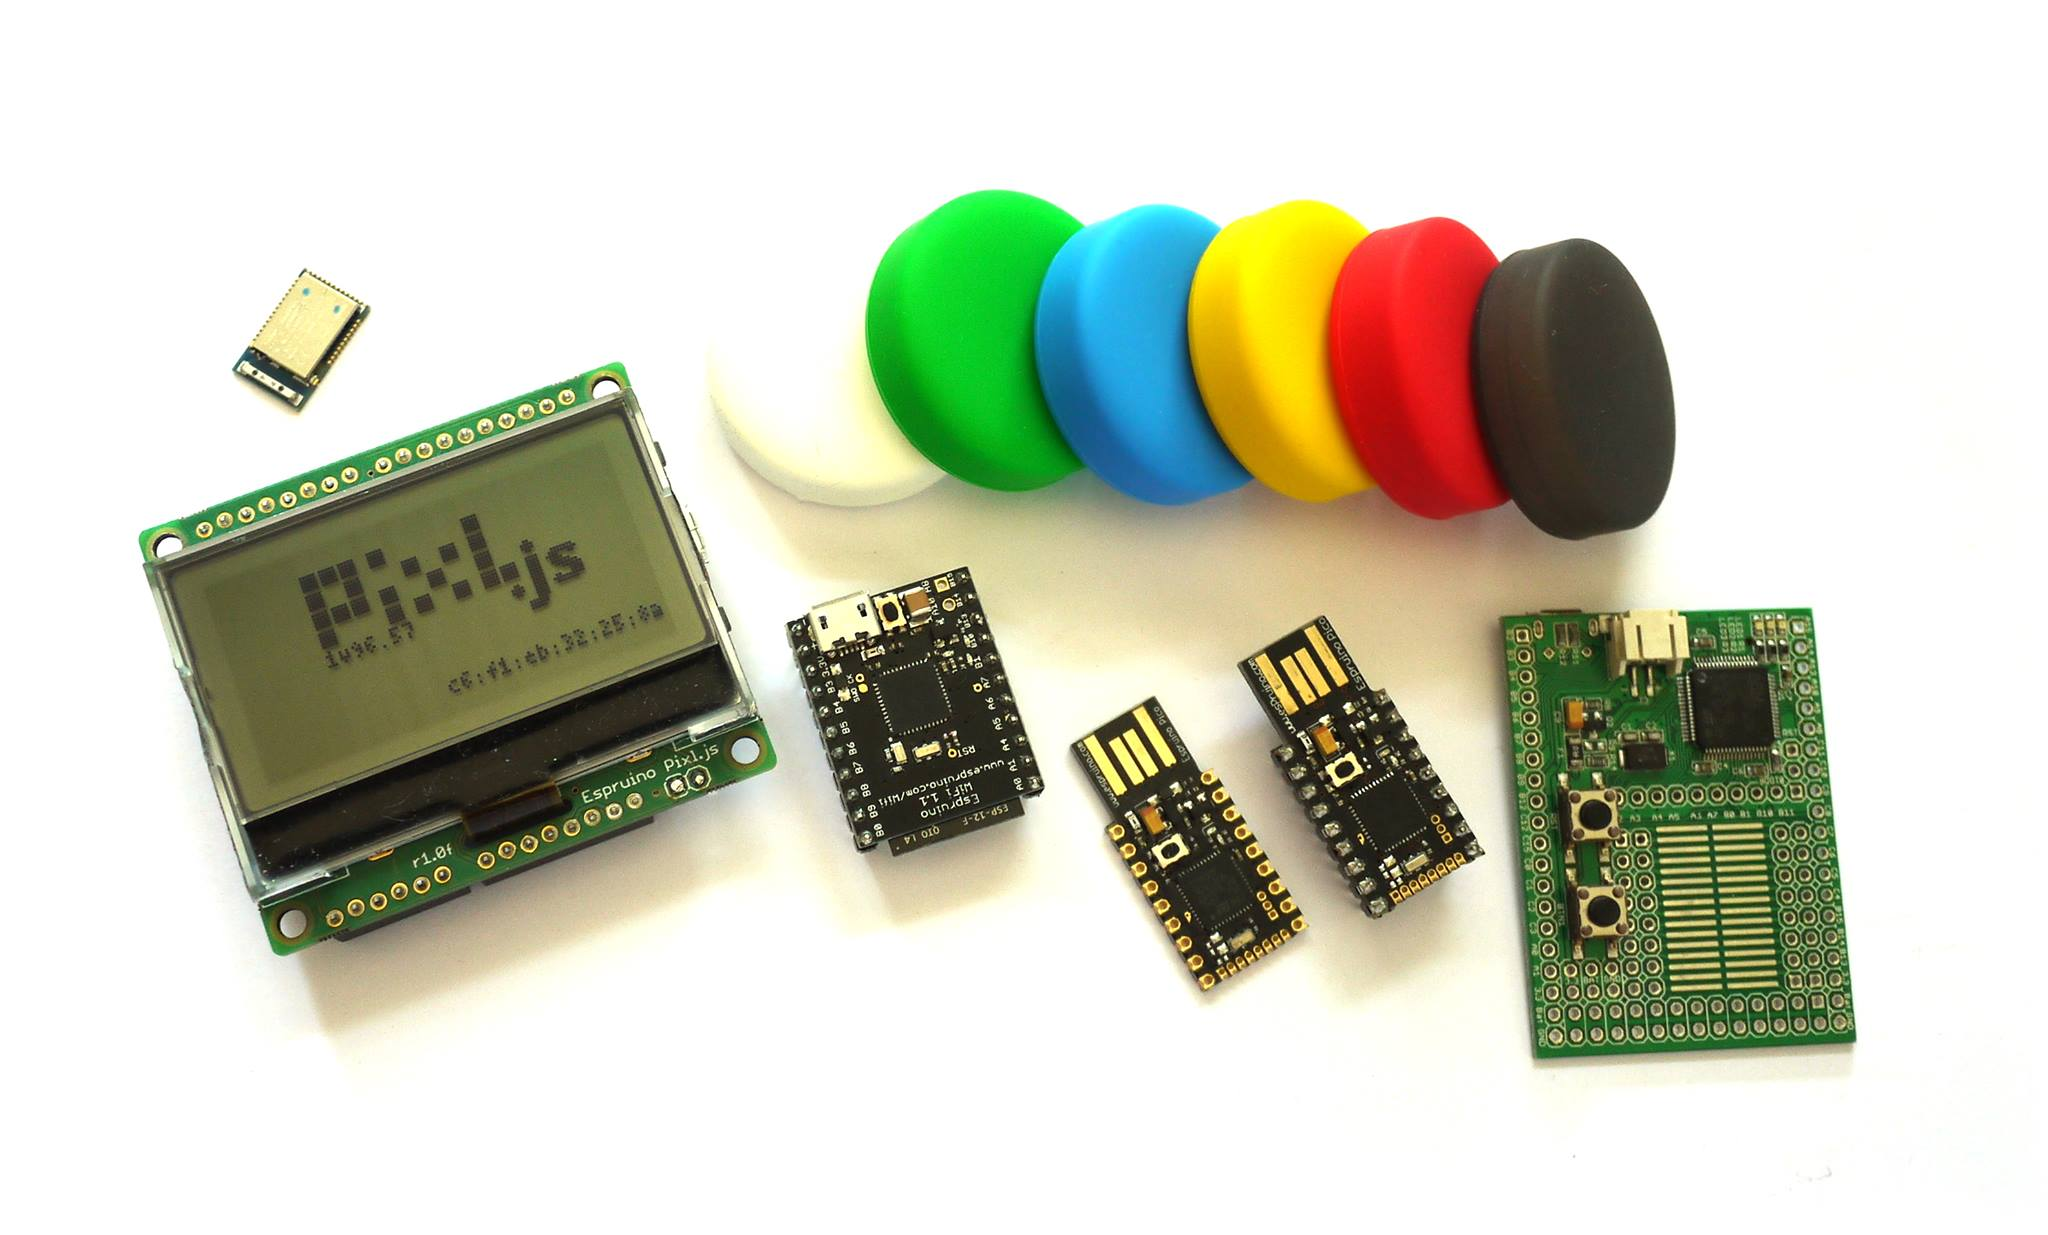
\includegraphics[width=10cm]{dissertation/images/espruino_devices.jpg}
    \caption{Espruino devices, Left to right Pixl, Breakout, Pico, Puck (in multiple colours), Pico(pinned and unpinned) and Original}
    \label{fig:espruinodevices}
\end{figure}
    
\subsection{UART}
\text Espruino devices communicate with the browser by utilizing the \href{https://erg.abdn.ac.uk/users/gorry/eg3576/UART.html}{UART protocol}, or Universal Asynchronous Receiver/Transmitter, a widely used communication protocol in the world of micro-controllers and embedded systems. It doesn't require a fixed clock rate between the sender and receiver and instead uses start and stop bits for data transmission synchronization. UART works by utilizing a transmission control line (TX) and a reception control line (RX); UART will begin by sending a start bit from TX to RX to initiate the start of a data transfer from here, data is transferred bit by bit over a single data line starting with the least significant bit (LSB) and finishing with the most significant bit (MSB) following this a stop bit is sent to signal data transfer has finished. This is detailed in figure \ref{fig:UART}.

\begin{figure}[!ht]
\begin{center}
    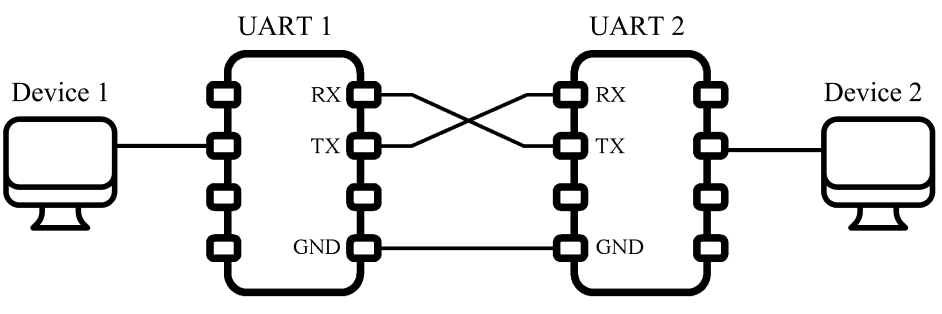
\includegraphics[width=10cm]{dissertation/images/UART_diagram.png}
\end{center}
\caption{UART diagram showing data flow between devices 1 and 2 via the UART controllers transmission and reception control lines}
    \label{fig:UART}
\end{figure}

\subsection{WebBluetooth}
\text UART connection with a web browser is facilitated via \href{https://developer.mozilla.org/en-US/docs/Web/API/Web_Bluetooth_API}{WebBluetooth}. WebBluetooth is an aspect of the JavaScript Web API that facilitates communication between web applications and Bluetooth Low Energy (BLE) devices. This technology allows web developers to control and access BLE devices using JavaScript, providing a streamlined and standardized approach.

WebBluetooth represents a milestone in integrating BLE devices into the web. It offers a common platform for web developers to interact with these devices, regardless of origin or operating system. It expands the possibilities for BLE devices, including the ability to control smart home technology or track fitness information through a web application.

\section{Package Development}

Software packages are methods of extending the functionality of a given language through externally written code. With the wide adoption of node.js in web development, many package developers have adopted the UNIX philosophy of building clean, modular, transparent, and robust code, \cite{TheArtOfUNIXProgramming}. This is achieved in modern web development through the Node Package Manager(NPM).

\subsection{NPM}
\href{https://www.npmjs.com/}{NPM} is a package manager for node.js. NPM is highly used within JavaScript programming to manage software packages. NPM provides an online hub for developers to search for relevant packages to aid their development process quickly. In addition, NPM encourages developers to share their packages and contribute to open-source initiatives. This tool is necessary for node development due to its extensive catalogue of packages and is required for contemporary JavaScript development.

\subsection{NPX}
\href{https://docs.npmjs.com/cli/v7/commands/npx}{NPX} (Node Package eXecute) is a package runner for the node.js environment, which allows for the execution of packages hosted on NPM's package repository. It allows developers to run packages without the requirement of installing a program globally on their systems. The package runner is highly utilised within environment-building systems such as React's \href{https://reactjs.org/docs/create-a-new-react-app.html}{create-react-app} due to its ability to provide a convenient method of running packages without having it install any other OS-specific package managers such as \href{https://brew.sh/}{Homebrew}.


\section{Device to device communication}
The challenge of real-time communication between devices in web development is a difficult subject. Despite this, real-time communication is widely used in web applications and mobile apps such as WhatsApp and Facebook Messenger for sending text data between two devices. Another aspect of real-time communication is sending voice data. The popular \href{https://developer.mozilla.org/en-US/docs/Glossary/VoIP}{Voice over Internet Protocol (VoIP)} is widely used by services such as Facetime or Discord. All of these products have an overarching theme of using either \href{https://developer.mozilla.org/en-US/docs/Web/API/WebSocket}{Web-Sockets} or \href{https://developer.mozilla.org/en-US/docs/Glossary/P2P}{Peer to Peer (P2P)} connection.

\subsection{WebRTC}
\href{https://developer.mozilla.org/en-US/docs/Web/API/WebRTC_API}{WebRTC (Web Real-Time Communication)} \text is an open-source project which extends the base functionality of JavaScript by supporting peer-to-peer data transfer between two web browsers without the need for external software. WebRTC uses signalling servers to initialise a connection between two browsers allowing for direct data transfer without additional server cost. This technology is highly effective in transferring data in the form of text, JSON, audio or video making it an ideal choice for video meetings or video game servers. Below in Figure \ref{fig:webRTC}, we can see the data flow between browsers and the signalling server.

\begin{figure}[!ht]
    \centering
    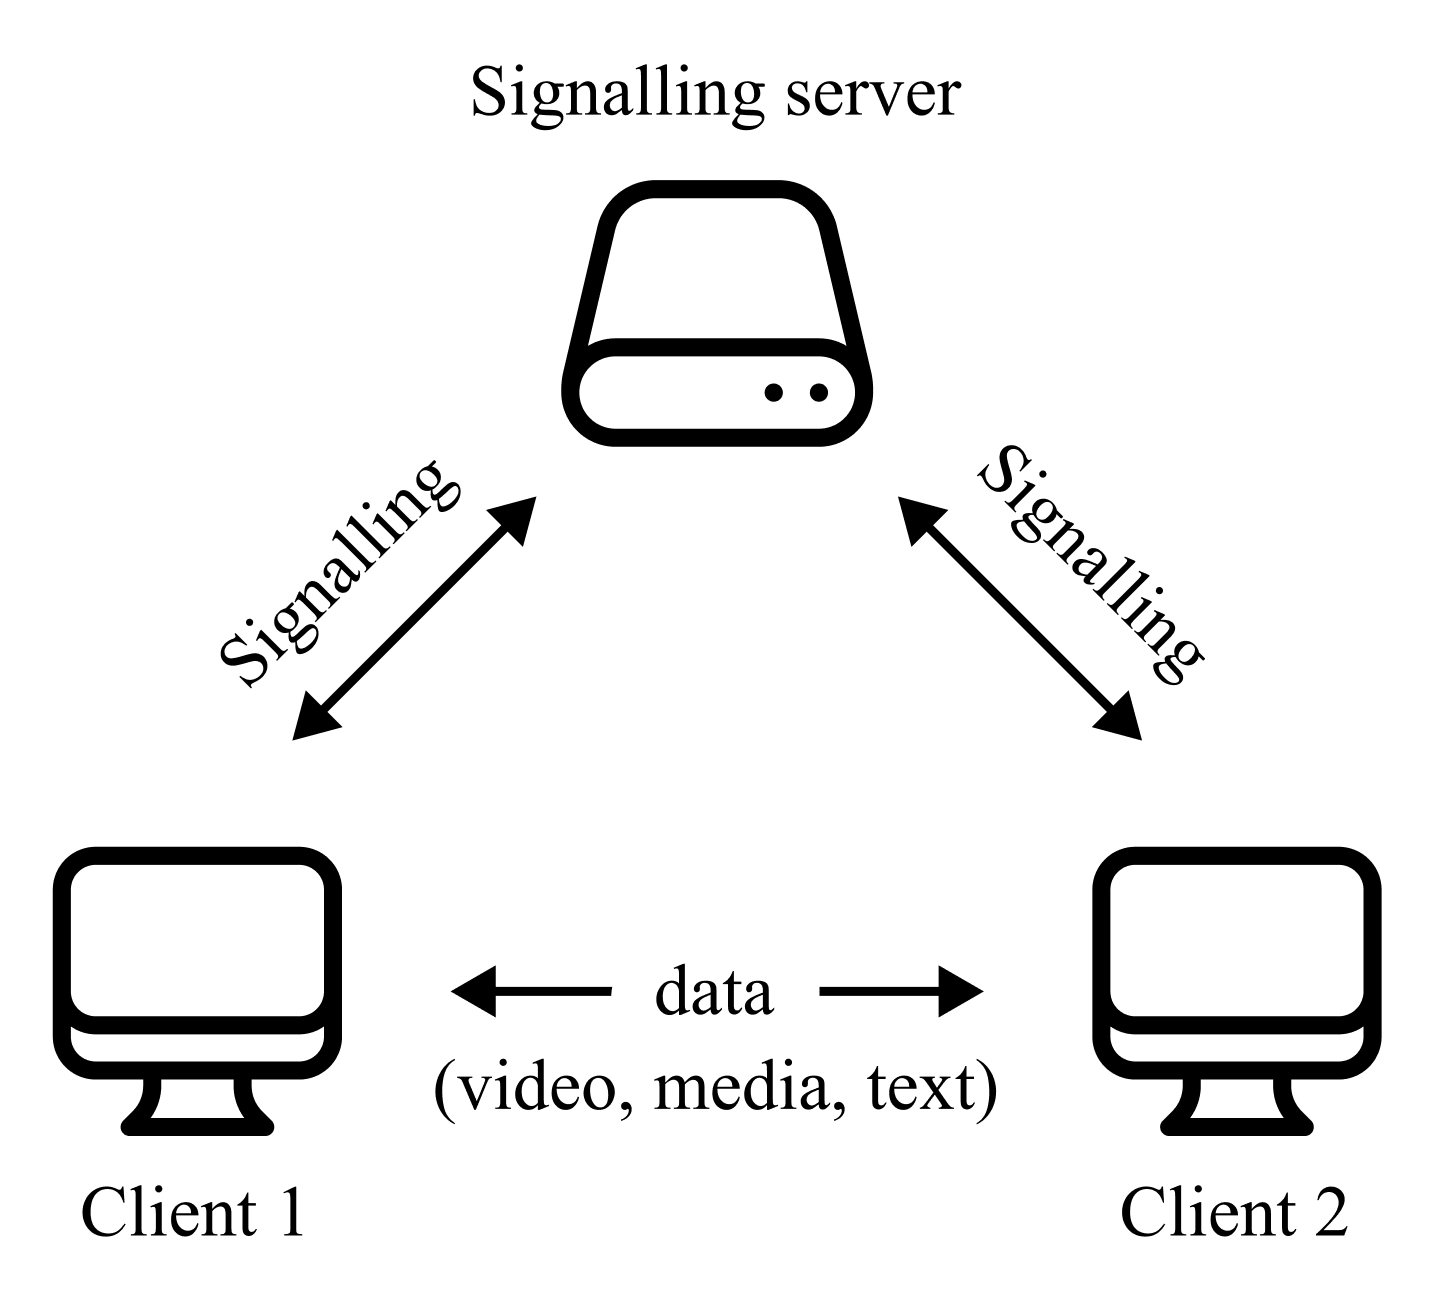
\includegraphics[width=5cm]{dissertation/images/web-rtc-diagram.png}
    \caption{WebRTC diagram showing the connection initialisation through the signalling server alongside the data transfer between two browsers}
    \label{fig:webRTC}
\end{figure}

\section{Open Source}

The Open source definition \cite{perens1999open} describes open source software as products where the consumers can freely; make and distribute copies of the software, make changes to the software’s source code and improve the software. Communities of contributors without any financial encouragement often maintain open-source projects. Many popular programming languages such as Python, JavaScript and Java are open-source projects with massive contributor pools allowing for the languages to improve to incorporate improvements from their user bases.

\section{Existing Projects}
\text The Espruino project is an ambitious attempt at bringing embedded systems programming to the masses through an easy-to-get-started ecosystem which takes advantage of many in-house tools to provide the best experience possible for the developers. These tools aim not to change the way we develop but extend upon it through the usage of the below tools we can see this approach.

\subsection{Espruino JavaScript language}
The \href{https://www.espruino.com/Reference#top}{Espruino native language} is an extension of the standard JavaScript library introducing embedded systems specific keywords such as \textit{SetWatch} and pin manipulation through the syntax \textit{PIN.method()}. Adding these keywords allows developers to interact and control embedded devices in a manner akin to alternatives such as Arduino or Micro Python. This extension of the language transforms JavaScript into a capable systems programming language aimed at Espruino microcontroller boards.

\subsection{Espruino IDE}
The \href{https://www.espruino.com/ide/}{Espruino IDE} provides an online platform for developers to get started working with their Espruino devices without the need to set up any local environments. This web application provides many features, such as device console logs and programming directly onto the device all around providing a perfect learning environment for new programmers and acting as an ideal debugging environment for more experienced developers.

\begin{figure}[!ht]
    \centering
    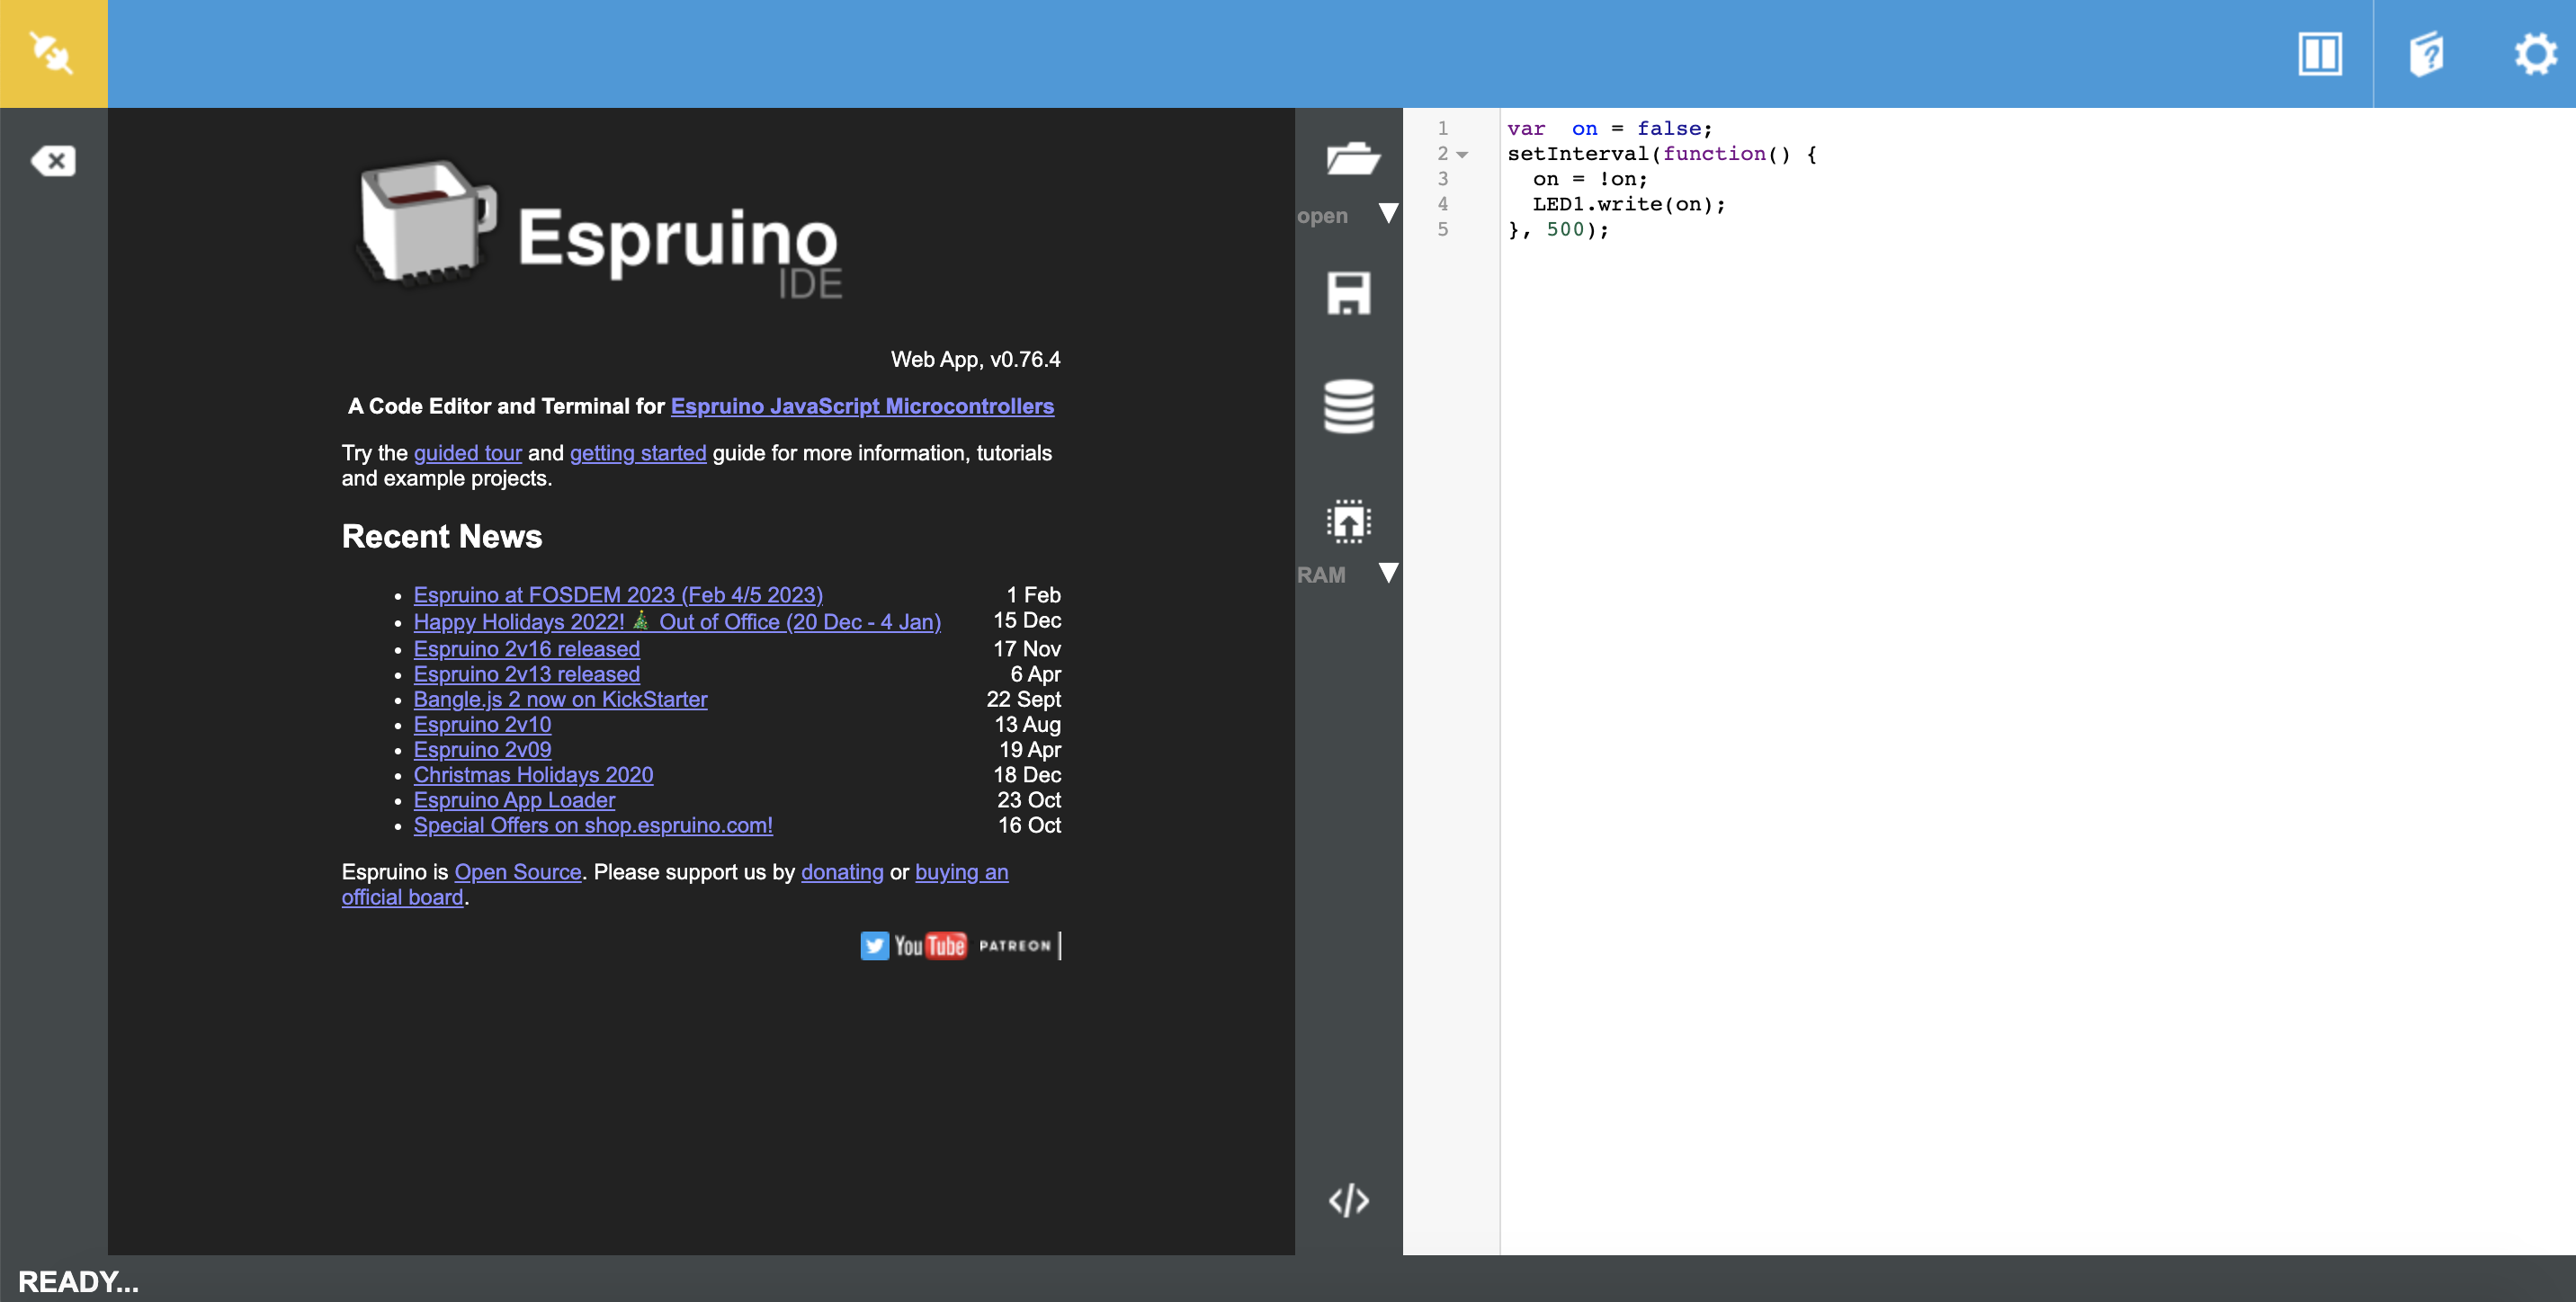
\includegraphics[width=12cm]{dissertation/images/espruino-ide.png}
    \caption{Espruino IDE homepage displaying the standard terminal and code editor side by side}
    \label{fig:espruino-ide}
\end{figure}

%==================================================================================================================================
\chapter{Analysis/Requirements}

\text Due to the nature of this project having multiple smaller packages/applications, these mini projects were analysed separately. A MoSCoW analysis \citep{waters2009prioritization} was undertaken on each project individually to accomplish this. Below is a compilation of the main points from this individual analysis, including overlapping themes and essential points from each project with the complete MOSCOW requirements for each project, referenced within Appendix \ref{appendix:MOSCOWAnalysis}.

\section{Problem specification}
\text The espruino platform provides an unopinionated approach to how users should work on their projects, resulting in a less-than-perfect catalogue of tools being utilised out of necessity. For beginners, these tools can be uninviting; alongside this, they lack an extensive tool library that may be useful to experienced programmers. When developing within the standard Espruino ecosystem of tools, there are areas where Espruino makes life harder for the developer; shown below, we can see some of the most prominent areas in need of improvement.

\subsubsection{Publishing information from the embedded device a webpage}\hfill\\
Espruino libraries such as UART.js lack the ability to return data on the Espruino devices, such as the code stored on the devices and return it to a webpage to be displayed or utilised for further development.

\subsubsection{Modular development}\hfill\\
Espruino development cannot work with JavaScript modules, meaning that  projects quickly become a massive unreadable file. 

\subsubsection{Code written as a string}\hfill\\
To write code to an Espruino device in the current implementation, all code must be within a string to allow it to be sent over a WebBluetooth connection. An example of writing code to an Espruino device is shown in figure \ref{fig:OLD_UART_DEVICE_WRITING_CODE}
    \begin{figure}[H]
    \centering
    \begin{minipage}{8cm}
        
    
        \begin{lstlisting}
            import UART from 'uart.js';
        
            let code = `setWatch(function () {
                    LED1.set();
                }, BTN, {
                    edge: 'rising',
                    repeat: true,
                    debounce: 50
                })`;

            UART.write(`${code};\n`);
            
        \end{lstlisting}
        \end{minipage}
        \caption{A code snippet that shows how device writing/communication is handled by UART.js}
        \label{fig:OLD_UART_DEVICE_WRITING_CODE}
    \end{figure}

     An additional issue with this approach is the requirement to end all code with a new line, as the interpreter will not execute the code otherwise. The code should be written as standard with code completion within the IDE. An example of how this could be done is shown in figure \ref{fig:NEW_DEVICE_WRITING_CODE}. An approach allows fewer errors at run time due to syntax highlighting. 

     \begin{figure}[H]
     \centering
    \begin{minipage}{8cm}
        \begin{lstlisting}
            import Device from 'new_package';

            let device = new Device()
        
            device.setWatch(function () {
                    device.LED1.set();
                }, device.BTN, {
                    edge: 'rising',
                    repeat: true,
                    debounce: 50
                })`;
            
        \end{lstlisting}
        \end{minipage}
        \caption{Proposed code snippet for how writing/communication should be handled without writing code as a string.}
        \label{fig:NEW_DEVICE_WRITING_CODE}
    \end{figure}

\subsubsection{Lack of code completion}\hfill\\
Another issue brought up through having to write code in a string is that no code completion is available during development, restricting developers from exploring available functionality from their IDE.


\section{Functional Requirements}
The problem statement made an open-ended approach to the current challenge possible by adopting a strategy to enhance existing products whilst building a platform enabling novice programmers to participate and learn. The following breakdown is the result of these considerations.

\subsection{Must Have}
\begin{itemize}
    \item A fully open-source ecosystem to allow for community contribution and overall clarity of how the project works at the code level.
    \item Clean and accessible syntax for the end developer to get started with, including inline documentation through IDE comments.
    \item Introduce a modular programming method to alleviate any confusion brought up by the current almost terminal-based approach of Espruino device programming to improve the development process.
\end{itemize}
\subsection{Should Have}
\begin{itemize}
    \item Support any style favoured programming style, including but not limited to JavaScript frameworks. A practice that will not discourage programmers at any level from jumping into something they are already familiar or comfortable with. This will include imports through script flags as well as NPM.
    \item Refined user interface to ensure integration into existing sites is not a hassle nor an eyesore. This should be consistent across all products.
\end{itemize}
\subsection{Could Have}
\begin{itemize}
    \item Easily extendable packages, including only the core functionality of the packages, to allow developers to extend and implement desired features without being held back by any limitations.
\end{itemize}
\section{Non-Functional Requirements}
\text As previously mentioned, the project aims to improve the Espruino platform whilst providing beginners with a platform to grow their programming skills. An important requirement is to produce an ecosystem of clear instructions and examples to follow along and fully understand the platform's capabilities.
\subsection{Must Have}
\begin{itemize}
    \item A well-populated documentation site to explain the features of each package in depth.
    \item A hub for users to explore in-depth projects built on the espruino-tools platform whilst allowing them to show off their creations to the public.
    
\end{itemize} 
\subsection{Should Have}
\begin{itemize}
    \item Easy contribution from the open-source community through the usage of modern standards and clear, clean code.
    \item A platform with online guides and videos which clearly walk the developer through the process of building a project allowing beginners to get started with functioning examples whilst letting them explore the intricacies of the package.
\end{itemize} 

\section{Specification changes}

\text As this project was very open-ended and heavily incorporated user testing, it allowed for an approach where feedback generated what was happening next. Through the development process, many smaller projects were built to improve the development experience; below are the significant changes to the original specification; each breakdown in the specification is expanded further through complete MOSCOW analysis within appendix \ref{appendix:MOSCOWAnalysis}.

\subsection{Peer to Peer}
\text During the development of the main package, a discussion occurred surrounding the limitations of the WebBluetooth API. As WebBluetooth is a new technology, the support for it is restricted; by viewing the \cite{caniuse} tool shown in figure \ref{fig:caniuse_webblue}, we can see that only Chromium-based browsers support this API with no direct support for iOS devices.

\begin{figure}[!ht]
    \centering
    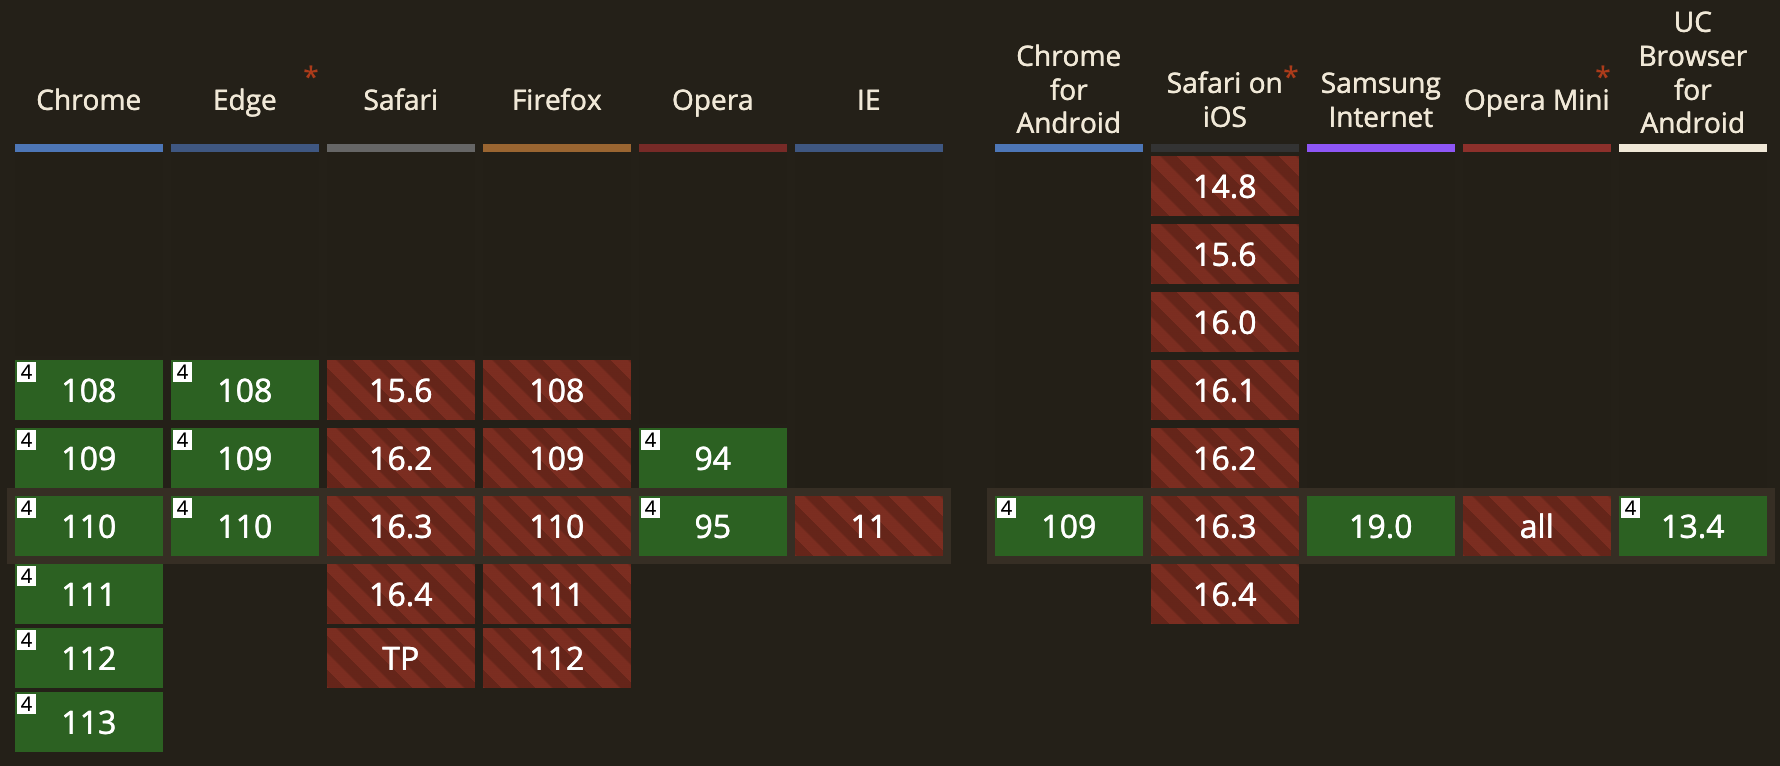
\includegraphics[width=12cm]{dissertation/images/caniuse_webbluetooth.png}
    \caption{Browser support comparison for the WebBluetooth API use by Espruino for UART connection to the browser from caniuse}
    \label{fig:caniuse_webblue}
\end{figure}

A problem this presents is that \cite{mobile-os-market-share}'s Mobile Operating System Market Share United Kingdom states that more than half (52.44\%) of smart device users are on iOS devices as shown in figure \ref{fig:smartdeviceusage}\\\\

\begin{figure}[!ht]
    \centering
    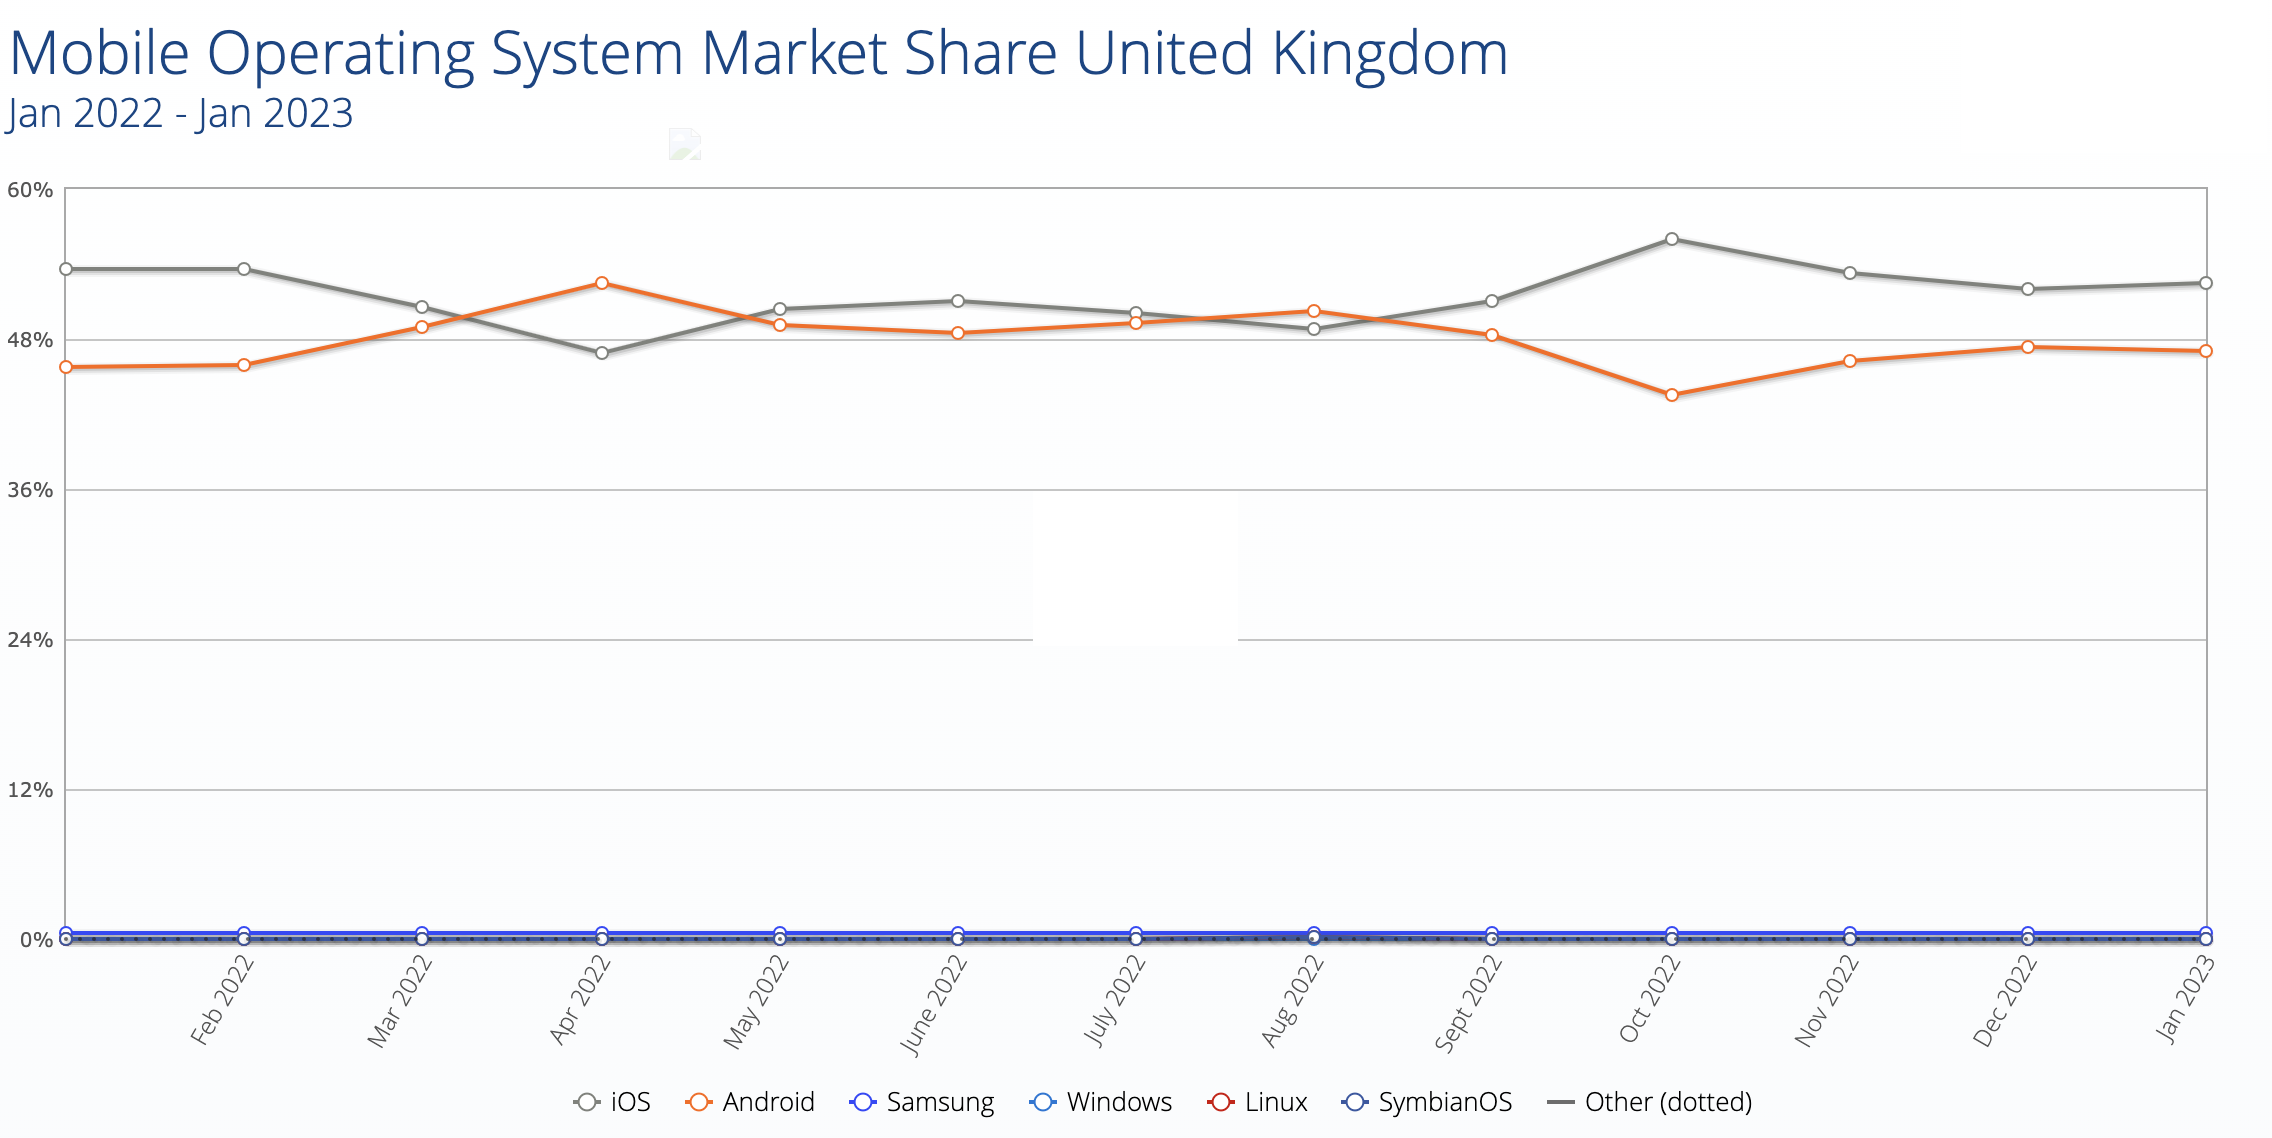
\includegraphics[width=12cm]{dissertation/images/mobile-operating-system-usage.png}
    \caption{Mobile Operating System Market Share United Kingdom (Jan 2022 - Jan 2023)}
    \label{fig:smartdeviceusage}
\end{figure}

Smartphones may be used within the remote embedded systems space due to the limitations of the embedded device. Mobile phones present multiple input and output interfaces that Espruino devices do not have, such as cameras (used in tracking), microphones (used in voice commands), or even touch controls that allow for a more comprehensive feature set than the simple buttons provided.
\\ 

To bypass this issue and allow unsupported control over these devices, a solution of utilising a peer-to-peer communication package was developed to allow unsupported devices to connect to a main supported device as shown in figure \ref{fig:mobile-computer-connection}. 

\begin{figure}[!ht]
    \centering
    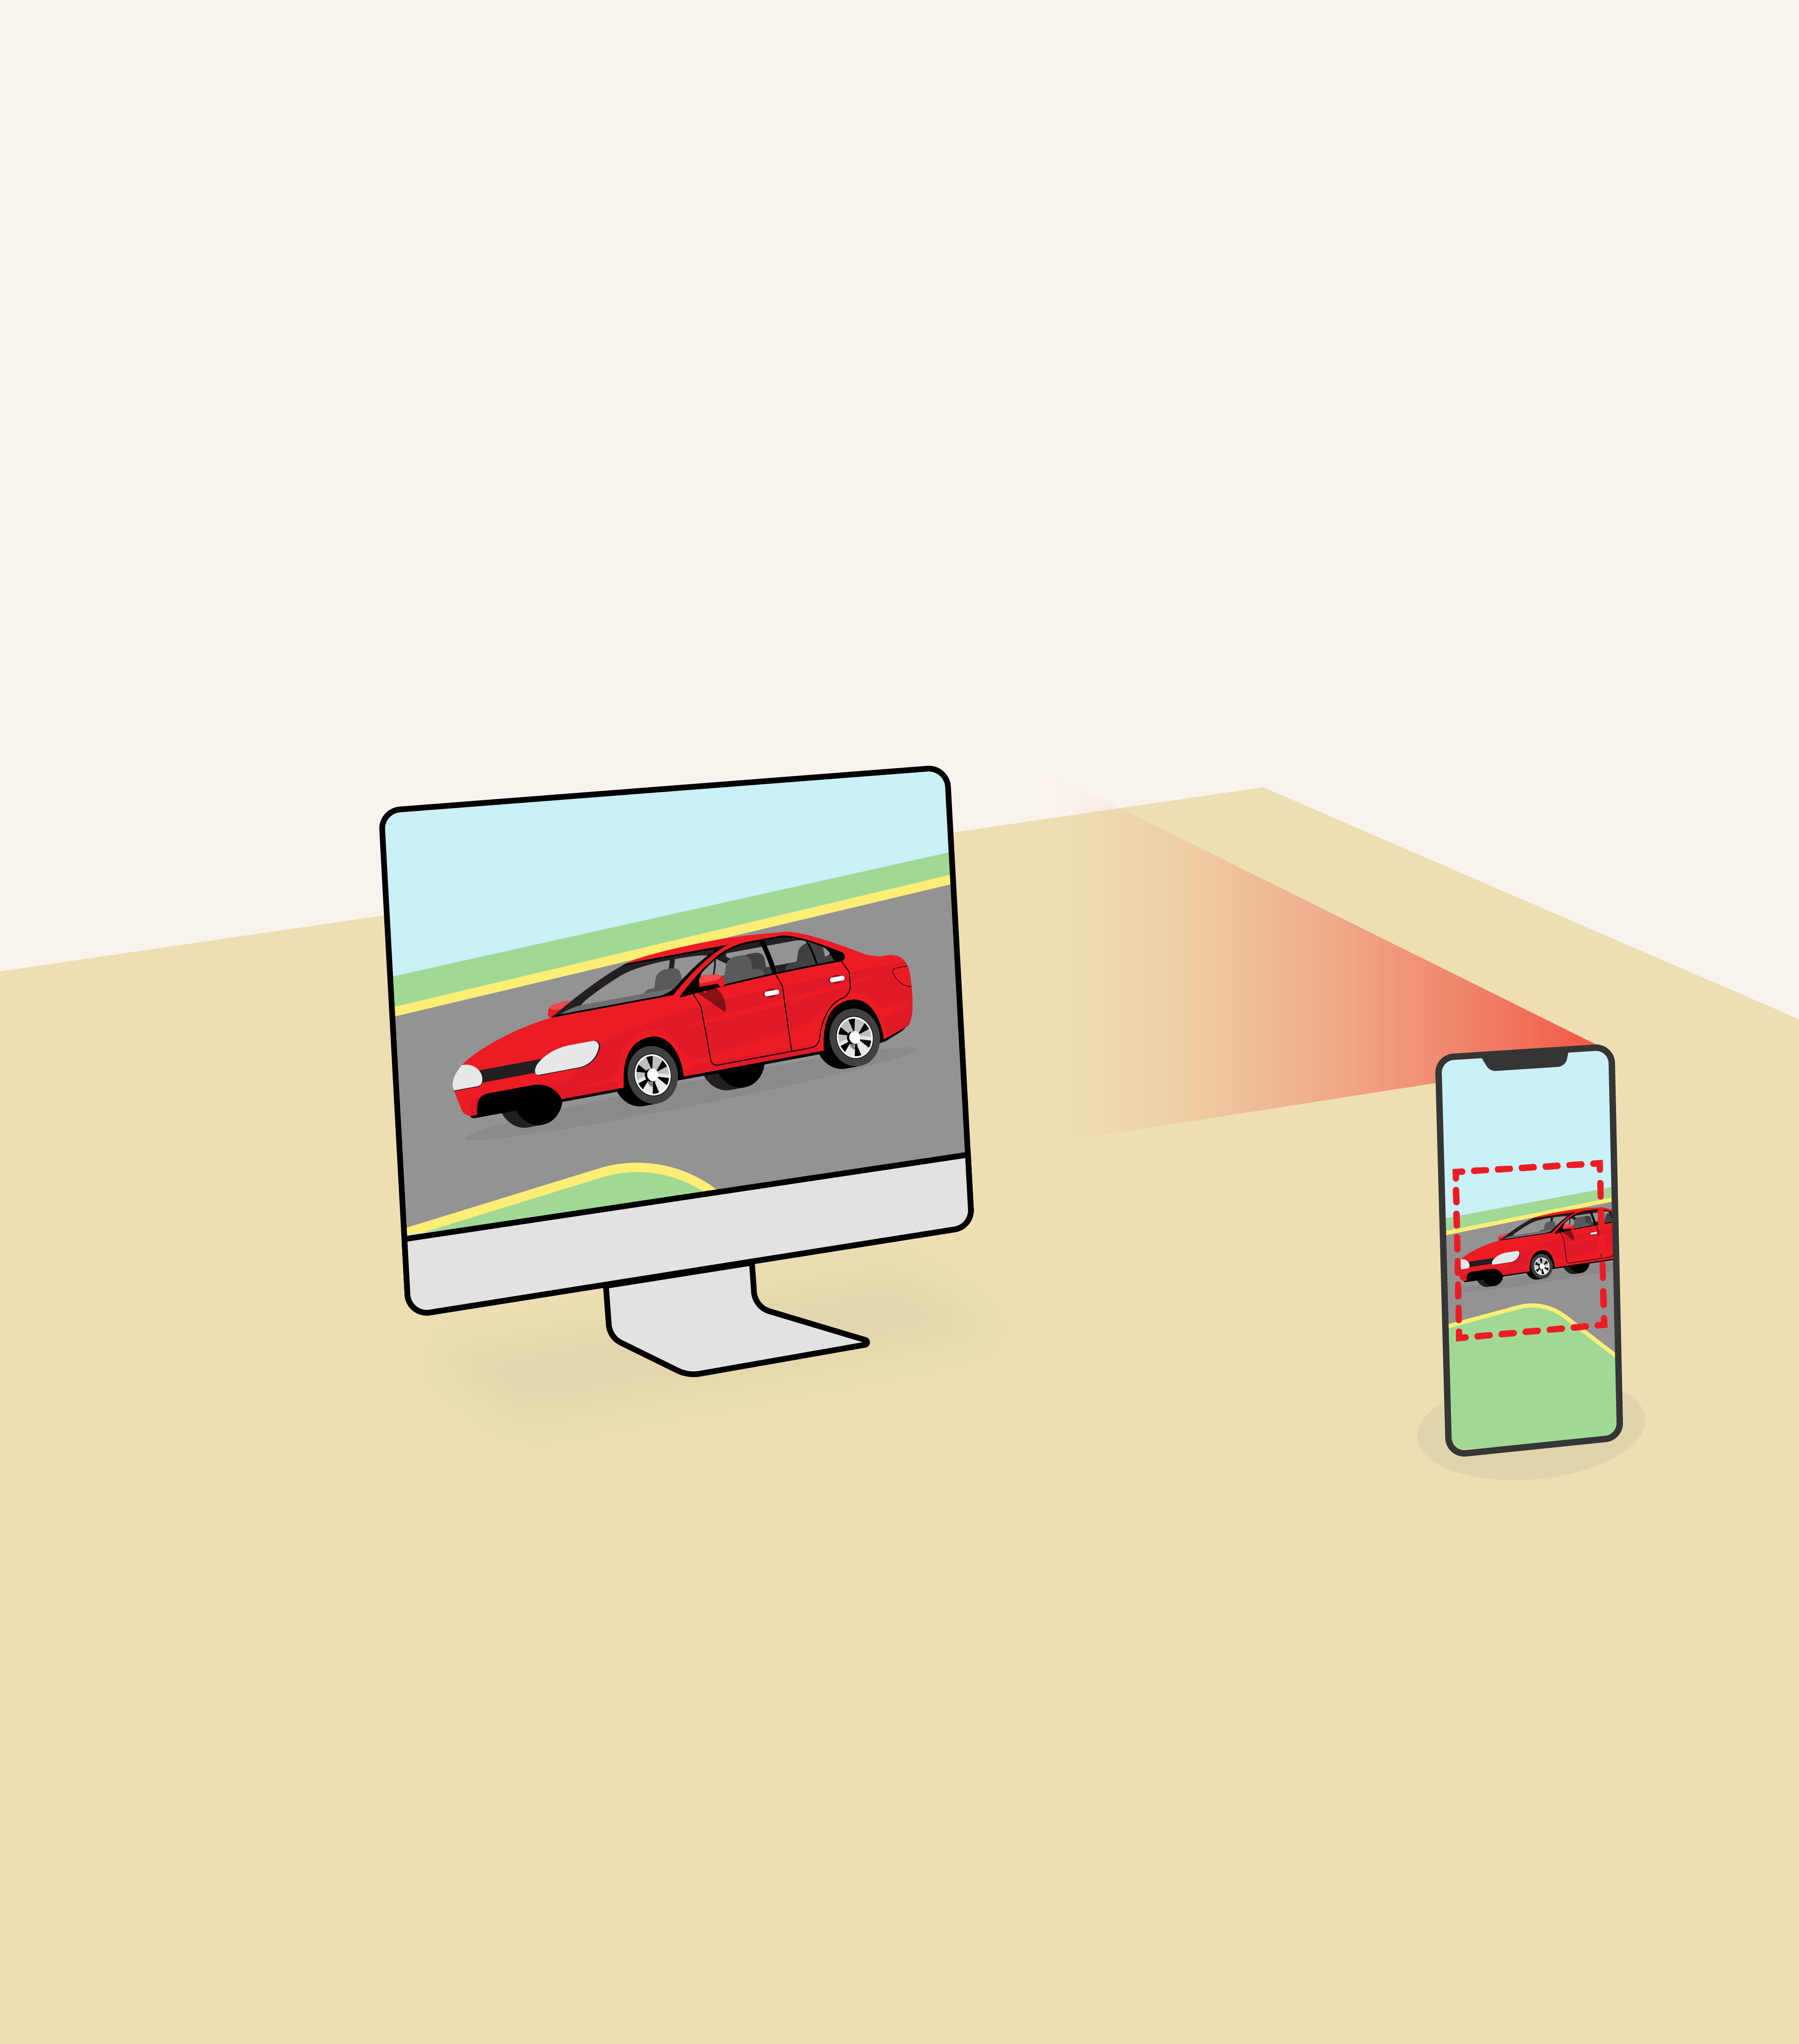
\includegraphics[width=7cm]{dissertation/images/mobile-computer-connection.png}
    \caption{The usage of a mobile device to control a web browser through the WebRTC connection via the camera}
    \label{fig:mobile-computer-connection}
\end{figure}

This approach was taken to allow users with iOS devices to control espruino devices, expanding the scope of projects available to a broader audience. To incorporate this, it would need to have the following specifications:
\\
\begin{itemize}
    \item Support for any mobile device type, including but not limited to iOS and Android devices.
    \item Simplify the peer-to-peer integration focusing on sending data and video whilst not restricting developer freedom.
    \item Utilise an automatically generated QR code to allow easy device connection through a mobile device's camera.
\end{itemize}


\subsection{Transpiler}
As the main project began to incorporate more complex behaviour like nested statements for anonymous functions which contain scope code within them. This presented an issue where the previous approach of a mini parser utilised a map of possible espruino methods along with string manipulation to replace known configurations that could come up. This approach had a few problems, such as no freedom to name instances of espruino devices as well as no support for the use of variables or nested scoped code. This approach to solving the problem ended up making the development experience worse, going directly against the aims of the project. The following code was not possible in the original approach.

\begin{lstlisting}
    import { Puck } from '@espruino-tools/core';

    let my_custom_puck_name = new Puck();
    
    my_custom_puck_name.onPress(async () => {
    
        let light_val = await my_custom_puck_name.getLightVal()
        
        if(light_val){
            my_custom_puck_name.LED.on("red");
        } else {
            my_custom_puck_name.LED.off("red");
        }
    })
\end{lstlisting}

To solve this problem, an approach which took inspiration from transpiled languages such as TypeScript made the most sense. A Transpiler, in this case, allowed a new language to be built extending JavaScript's syntax; this could then be compiled into plain JavaScript, which Espruino's compiler could interpret. For the transpiler to be effective, it had to ensure to incorporate the following criteria.
\\
\begin{itemize}
    \item successfully converts all standard JavaScript allowing for variable declaration, nested scoped code, and imports/exports.
    \item Allow for code written in either standard Espruino language or the new Espruino tools syntax for niche unsupported methods not to be restricted.
    \item Support modern JavaScript programming including modules, classes and syntax such as arrow functions or async/await in-line with \cite{kolce2018javascript}.
\end{itemize}

\subsection{NPX Tool}
\text By expanding the espruino platform to the NPM platform, it became apparent that the setup of the package directory may become cumbersome for more experienced developers or downright difficult for beginner programmers with no previous node.js knowledge. By taking inspiration from React's \href{https://reactjs.org/docs/create-a-new-react-app.html}{create-react-app} tool, it made the most sense to approach the problem in the same way by allowing users a simple command line prompt with avid customisation to allow a default project which fits the needs of most developers leaving heavily customised projects to the audience of people that needed it. An example of how React achieves this can be seen in figure \ref{fig:create-react-app}.
\begin{figure}[H]
    \centering
    \begin{lstlisting}
        npx create-react-app test-app --template typescript
    \end{lstlisting}
    \caption{The terminal command utilised to start a react project prepared with typescript.}
    \label{fig:create-react-app}
\end{figure}
\text To incorporate this, it would need to have the following specifications:
\begin{itemize}
    \item Create a working directory to allow users to get started directly after the command is run with no additional setup.
    \item An effective build command to convert users' node.js project into its respected static files for easy hosting and sharing of projects.
    \item Support for different JavaScript development approaches, including frameworks such as React and Vue or just plain JavaScript solutions such as vanilla JavaScript or TypeScript.
\end{itemize}

\subsection{Online Environment}
\text The original Espruino project includes an online environment which allows users to develop straight onto their Espruino devices, removing the need to set up a local environment to test smaller features. As this project utilises a new syntax whilst bringing many useful development tools, such as gathering device code effectively, it made sense to take inspiration from the Espruino IDE and create an environment which supports this new style of programming on Espruino devices whilst incorporating functionality aimed at improving the experience for developers. For this aspect of the project to be effective, it had to meet the following criteria:
\\
\begin{itemize}
    \item It must support live development with the ability to run code and see device output to allow developers to catch any bugs that may be missed in standard development.
    \item Bring the ability for users to upload and download their code to allow easy integration into a larger project, be that through debugging or just testing features first before bringing them into the project.
    \item Allow users to directly see device code in a read-only code editor, improving developers' debugging experience.
\end{itemize}

% Allow users to have an environment in which they can test new features without setting up a whole development environment. This can be used to test functionality or even develop whole projects.
%==================================================================================================================================
\chapter{Design}

\section{Development}

Throughout the development of this project, multiple development approaches have been taken based on the project style. By utilising both a feedback-driven model alongside a test-driven approach, each aspect of the project has been allocated an appropriate development style to ensure robustness, cleanness and adequate feature sets. Agile methodologies enforced these approaches by dividing specification points into work items and allocating them during week-long sprints, furthering the quick approach to iterating the product.

\subsection{Feedback Driven Development}
By utilising a feedback-driven approach, the project was able to evolve constantly into a product more suited to the people actually using it. To take full advantage of the Espruino community and ensure the project provided useful features, three methods of gathering feedback were used.

\text \\

\subsubsection{Espruino Forum}\hfill\\
The Espruino Forum pictured in figure \ref{fig:espruino-forum} is a platform used by the community to share new projects or to ask for help with problems run into within the development cycle. The forum allowed for direct communication with Gordan Williams, the creator of the Espruino platform. Discussion and feedback on the shared project allowed for further iterations of the project to be made.

\begin{figure}[!ht]
    \centering
    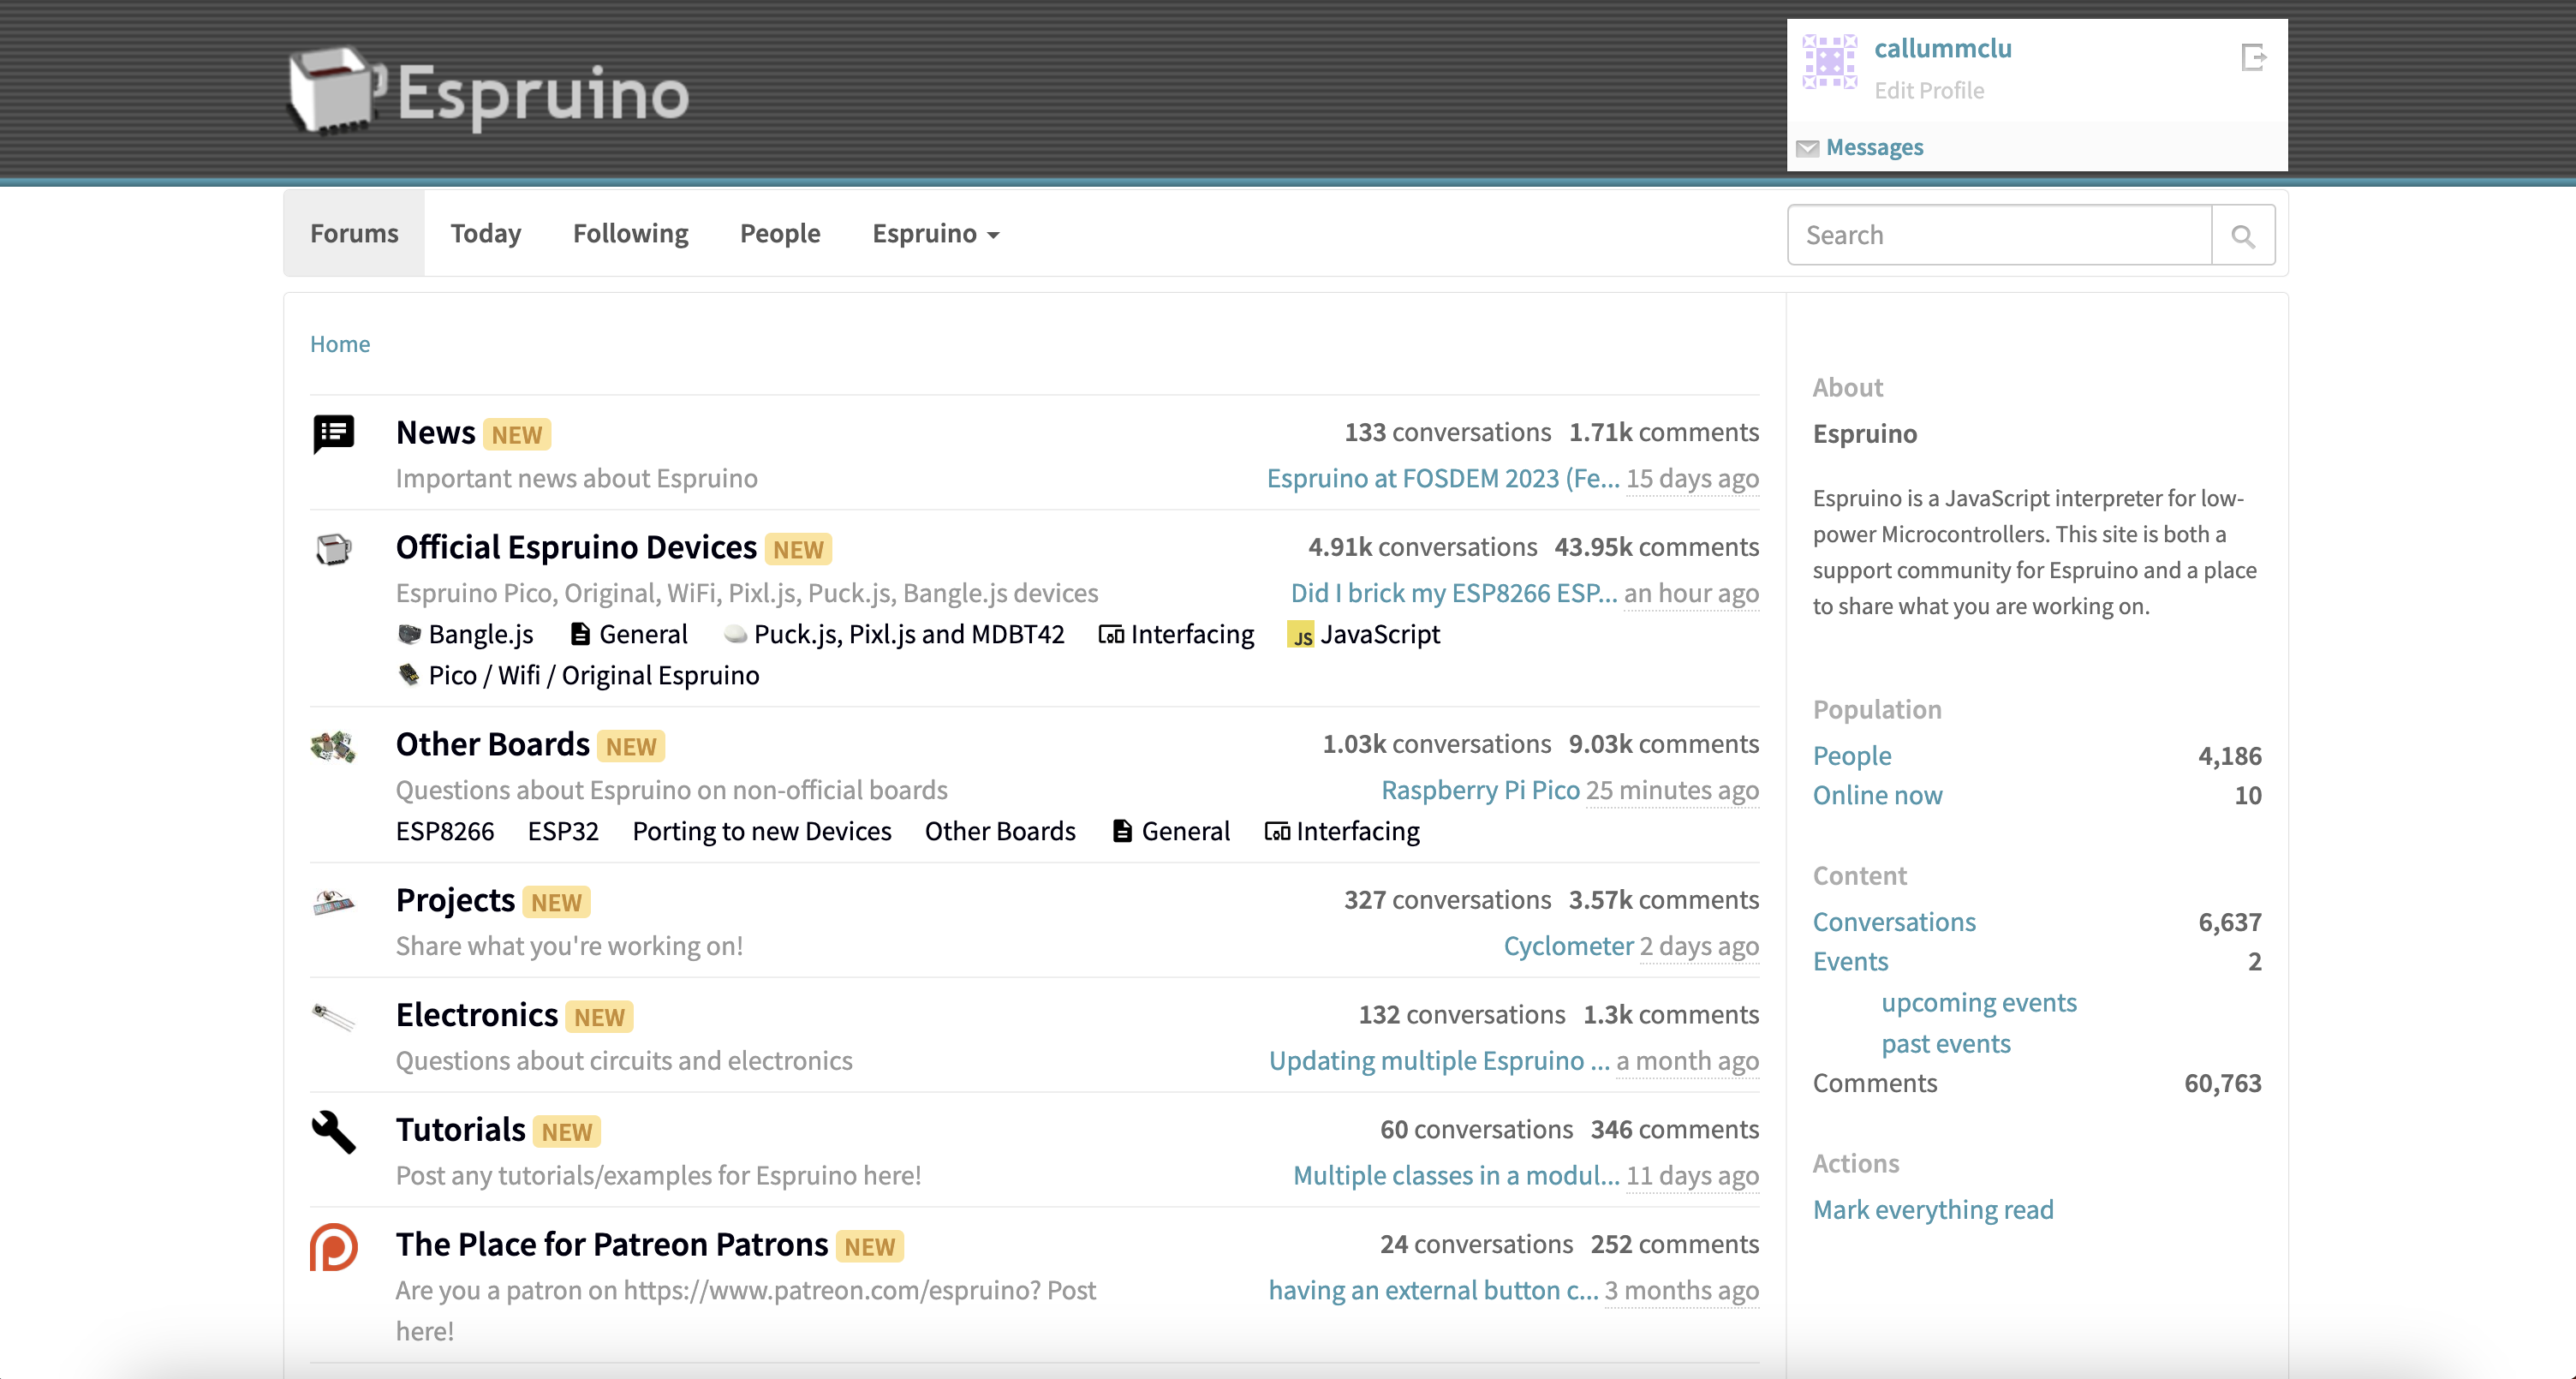
\includegraphics[width=12cm]{dissertation/images/espruino-forum.png}
    \caption{Espruino Forum, a community to ask questions or share your project}
    \label{fig:espruino-forum}
\end{figure}

\text \\
\subsubsection{User testing}\hfill\\
Throughout the full project user testing was utilised allowing a constant flow of feedback from a developer using the packages to build their own substantial project utilising every aspect of the package suite. By incorporating this feedback this vital stage allowed for package-wide user testing as well as both suggestions for feature additions and help with finding bugs within the code.

\text \\
\subsubsection{Supervisor Feedback}\hfill\\
Due to the supervisors' involvement within the Espruino ecosystem through the development of a new espruino device as well as a genuine interest in the products feedback from them was essential. By having somebody who knew about the platform and had an acute interest in the product themselves allowed for many discussion sessions where new features and ideas could be bounced back and forth allowing for a creative environment including new direction ideas or even how features could be improved.

\text \\

This approach allowed for very small iterations to be planned out developed and deployed in a very short period further allowing again for quick feedback surrounding the changes as well as a platform to test prototyped ideas as a smoke test for the final product.


\subsection{Test Driven Development}

Test Driven Development (TDD) is the process of writing failing tests first and ensuring the criteria are met before writing the following tests until the end product is produced. Where possible Test Driven Development was used throughout the full package ecosystem. For all packages, the feedback-driven approach was used in tandem with test-driven development to ensure these feature-rich packages both did not break with massive changes as well as allowing them to maintain substantial test coverage. Overall this approach allowed for the code quality to be constantly improved without worries of breaking previous functionality and played a vital part in the development of the transpiler package and its conversion from the imperfect original core implementation.

\section{Organisations}

By utilising organisations within this project I was able to keep relevant code in a single place; this was important due to the open-source nature of the project by keeping everything together users or contributors are able to navigate the full code base with less hassle.

\subsection{GitHub}
The GitHub platform is widely used within the open-source community, a feature provided by GitHub is GitHub organisations. GitHub organisations provide a workspace that promotes contribution and collaboration through allowed permissions allowing for control over who has access to alter code. 

\text Alongside this Github organisations allows for a project with multiple repositories to be grouped together keeping all relevant code in one place. Doing this allows newer developers to discover both how all the packages work and also see the catalogue of packages offered by the ecosystem. Below in figure \ref{fig:ghorg} we can see the GitHub organisation for this project.

\begin{figure}[!ht]
    \centering
    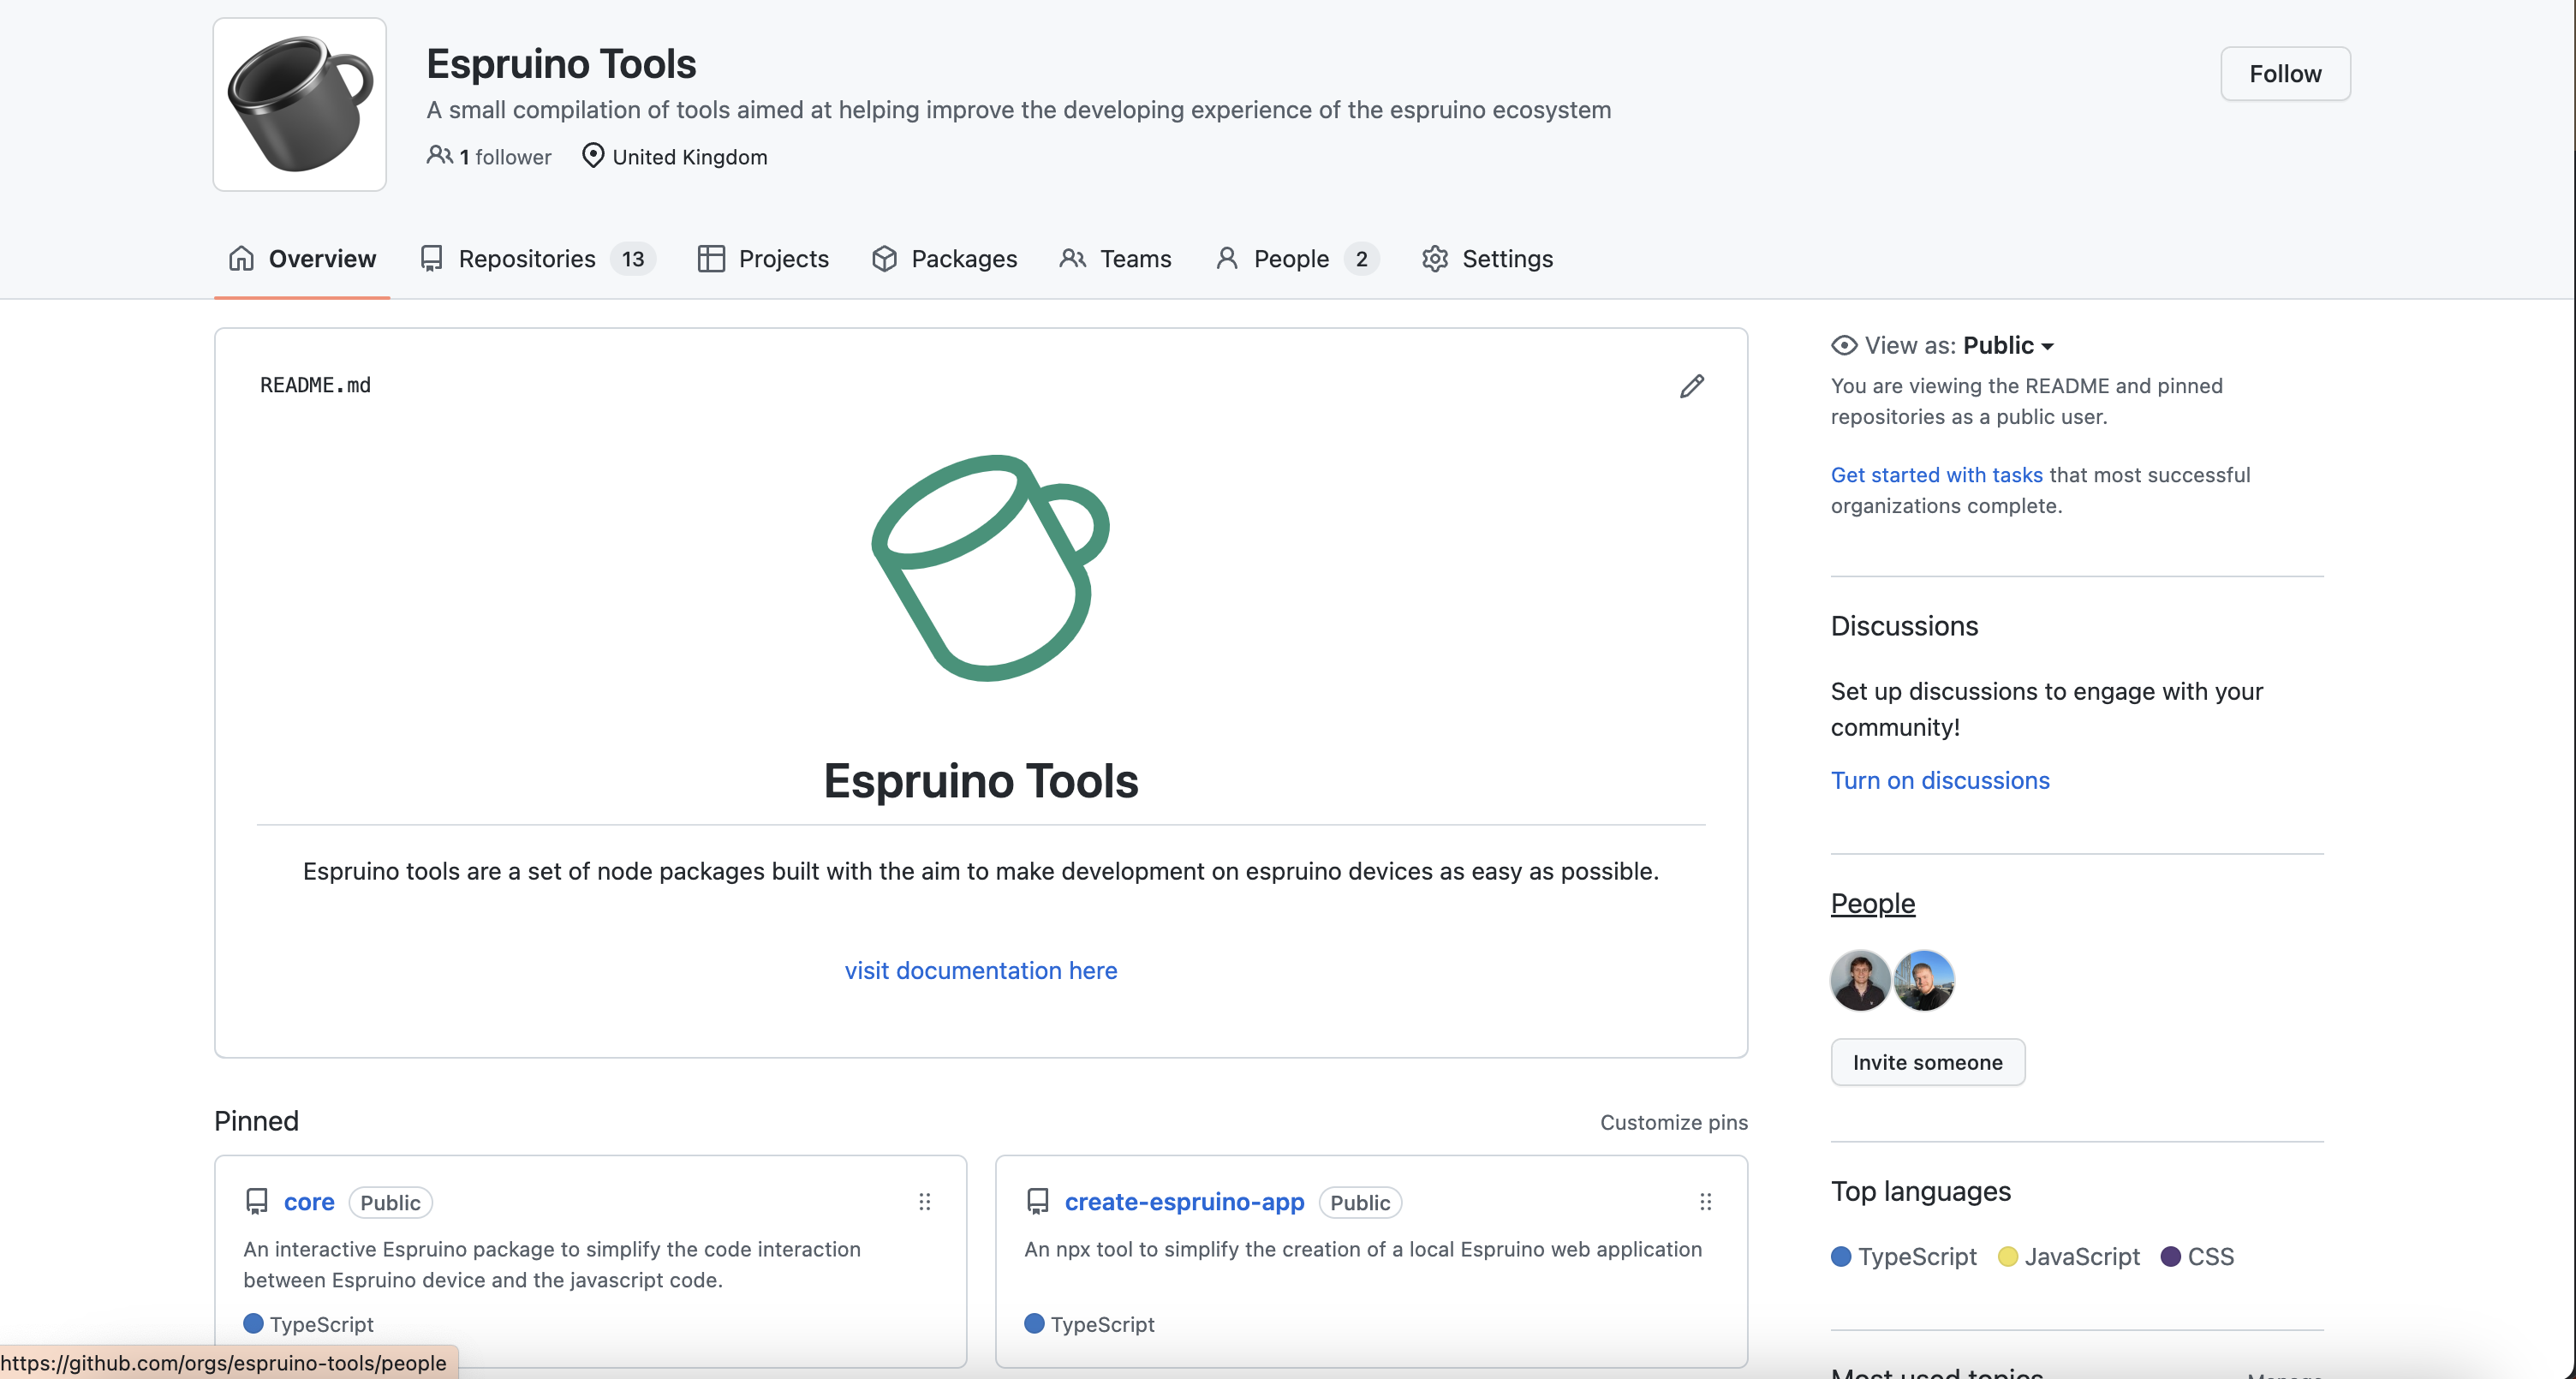
\includegraphics[width=10cm]{dissertation/images/github-organisation.png}
    \caption{\href{https://github.com/espruino-tools}{Espruino Tools}' Github organisation splash page with the most popular packages displayed}
    \label{fig:ghorg}
\end{figure}

\subsection{NPM}

NPM provides a solution similar to GitHub organisations through scoped packages. NPM's scoped packages provide similar benefits such as keeping related code together whilst adding others. One of the main draws to NPM's scoped packages is the ability to name your packages similarly to packages that have previously been built prepending a given organisation's name. This approach avoids cryptic package naming schemes whilst keeping the projects consistent. As seen below in figure \ref{fig:npmorg} each scoped package within the organisation maintains the syntax of \textbf{@espruino-tools/<package-name>}.

\begin{figure}[!ht]
    \centering
    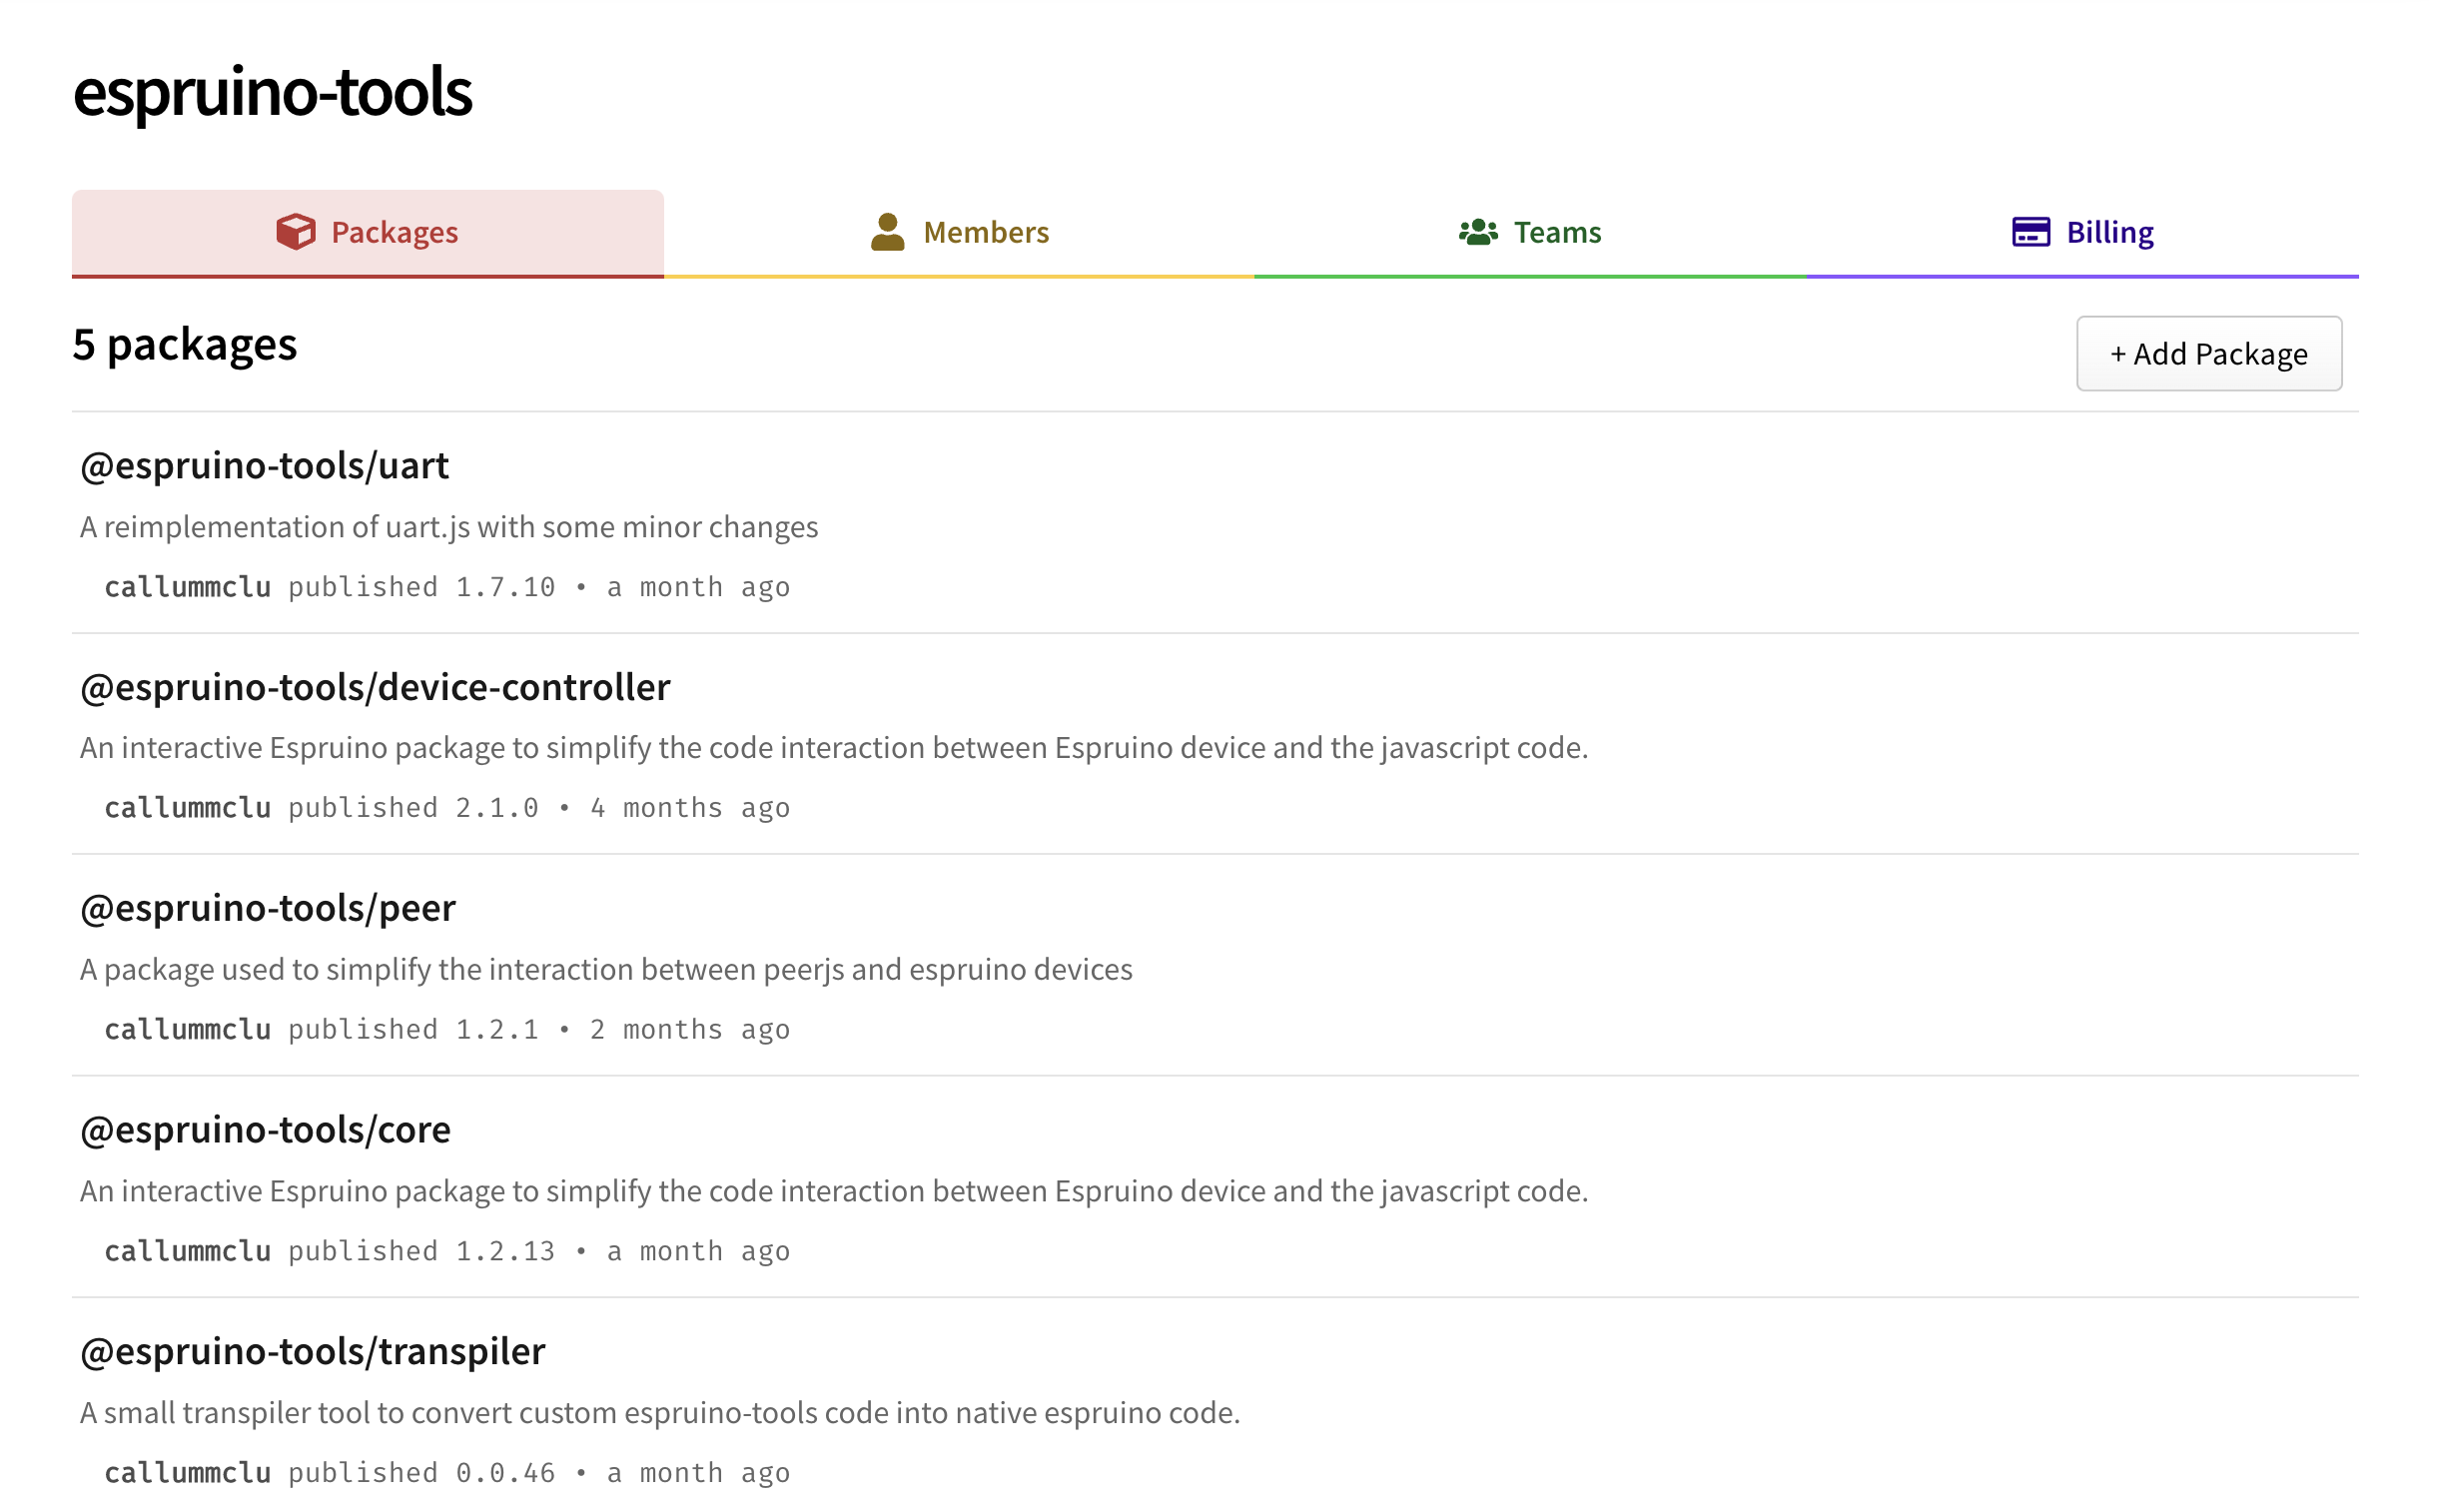
\includegraphics[width=10cm]{dissertation/images/npm-scoped-packages.png}
    \caption{Espruino Tools NPM package Organisation showcasing the UART, Peer, Core and transpiler as scoped packages alongside the depreciated device-controller package previous used as the core package}
    \label{fig:npmorg}
\end{figure}

\section{Packaging Naming scheme}
A massive factor when developing NPM packages is how to correctly name them to both provide context for functionality without adding additional confusion. Whilst developing the package ecosystem 2 main questions arose, how can we group packages together and how do other successful package ecosystems do this? As previously stated in the sub-section 4.2.2 NPM's scoped packages allowed for a clean and clear representation of package grouping through the organisations' name, this solved this issue. Following this further research was done into successful package ecosystems such as \href{https://babeljs.io/}{babel}, \href{https://jestjs.io/}{jest} and \href{https://sentry.io/welcome/}{Sentry}. From this research, there seemed to be a clear unspoken naming convention for NPM packages this included.
\begin{itemize}
    \item \textbf{"core"} name for the main package.
    \item short descriptive package names, usually a single word when appropriate.
\end{itemize}

The criteria provided from this research provided clear instructions on how the packages within this ecosystem should be named.

\section{Package Versioning}
To ensure the package was versioned correctly, resulting in a reliable and secure experience for the end users an approach was taken from \citep{NPM-package-versioning}. This approach is shown in figure \ref{fig:NPM-versioning}

\begin{figure}[!ht]
    
\begin{center}
\begin{tabular}{|p{2.25cm}|p{7.25cm}|p{3.25cm}|}
 \hline
 \textbf{Update Type} & \textbf{Example Change} & \textbf{Version Change} \\
 \hline
 \hline
Bug Fix & Package updates or security fixes  &  x.x.1  \\
 \hline
Minor change & Non breaking additions such as functionality extension  &  x.1.x  \\
 \hline
Major change & Breaking changes such as changes in syntax, anything that is not backwards compatible  &  1.x.x  \\
 \hline
\end{tabular}
\end{center} 
    \caption{Criteria used to consistently version NPM packages based on the severity of the change split into bug (for small fixes such as bug or security patches), minor (for non-breaking feature additions), and major (for breaking changes that are not backwards compatible with prior versions)}
    \label{fig:NPM-versioning}
\end{figure}

\section{NPX Tool Repositories}
The NPX Tool aimed to generate directories based on a user's needs and aims to provide a wide variety of options to facilitate this. After exploring how React's \textbf{create-react-app} approached this problem we can see the team has opted to have directories for the \href{https://github.com/facebook/create-react-app/tree/main/packages/cra-template}{plain javascript implementation} and the \href{https://github.com/facebook/create-react-app/tree/main/packages/cra-template-typescript}{typescript implementation}. This dynamic approach provided by React's \textbf{create-react-app} inspired the design of the \textbf{create-espruino-app} in the following ways.

\subsection{Git sub-modules}
Whilst the \textbf{create-react-app} tool kept its templates within the same repository I believed this was a restrictive method and provided many downsides one of which being a bloated repository making it more difficult for developers to fully understand how the tool worked. To resolve this issue an approach using git sub-modules was taken. Git sub-modules allow for incorporating separate git repositories within one another; this would allow for the NPX tool repository to be linked to separate template repositories.

By using a single repository per template we are able to update file structure, patch security bugs, and package dependencies and even change the best methods of approaching building the web app without having to re-publish the tool. This approach also allowed for branching to be used for further flags on templates such as \textit{--clean-install} or \textit{--peer} meaning the end product would have a cleaner setup with more readable repositories.

\subsection{Flags}
Within CLI tool development CLI flags are used to provide user input and customise the output of a command. In the case of the tool developed CLI flags are proposed to provide the end developer with as much control over their new project as possible by incorporating different templates for popular web frameworks, easy access to a functioning setup of the peer package and even options for advanced allowing them to start off with a clean slate. These tags consist of:

\subsubsection{template}\hfill\\
The template tag allows developers to get started with a template built with one of 4 options: Plain Javascript, TypeScript, React or Vue. These options were chosen due to consideration from figure \ref{fig:js_framework_lib_comp} whilst maintaining the need for plain javascript/typescript templates to allow for flexibility when not working with a framework. The template tag allows for package-specific formatting to be set up by default this could be routing or general file structure.



\subsubsection{peer}\hfill\\
The peer tag allows users to get started with the peer package without having to worry about the restrictions of the WebRTC API such as SSL requirements or separate pages needing to be hosted for it to function properly.



\subsubsection{clean-install}\hfill\\
clean-install is a flag which is aimed at not restricting the usage of the tool to just beginners by allowing a directory to be populated just by the required packages removing any example splash pages presented by the standard package. The goal of this flag was to not alienate more advanced programmers whilst still giving them the benefits of the tool.

\section{UI/UX Improvements}
Previous implementations of device connection through packages such as \href{https://www.espruino.com/UART.js}{uart.js} all fall short when it comes to user experience presenting users with a badly designed modal with little to no control for leaving the modal without processing a request first. To tackle this problem with inspiration from the react component library \href{https://mantine.dev/}{Mantine} a Figma prototype was prepared to improve the user interface and experience of the mandatory modal. In figure \ref{fig:connection-modal} on the left we can see the old design with layout issues and a general lack of responsive design. In figure \ref{fig:connection-modal} we can also see the newly thought-out design prototype on the right incorporating an option to close the modal with a clearer design. 

\begin{figure}[!ht]
  \centering
  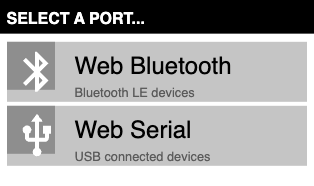
\includegraphics[width=6cm]{dissertation/images/old-modal-design.png}
  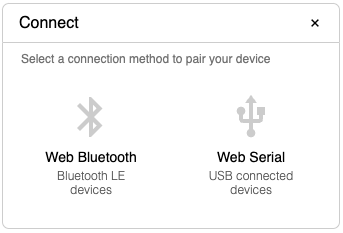
\includegraphics[width=6cm]{dissertation/images/new-modal-design.png}
  \captionof{figure}{Connection Modal comparison with the old connection modal(left) with stylistic errors and the new proposed connection modal(right) with modern styled based on Mantine component library}
  \label{fig:connection-modal}

\end{figure}

This design process incorporated the previously mentioned feedback-driven approach going through many iterations to reach a final product with feedback from my supervisor who had previously mentioned issues with the prior connection modal. Further wireframes can be found in appendix \ref{appendix:wireframes}


%==================================================================================================================================
\chapter{Tools / Technologies}

This project was heavily dependent on the tools and technologies used within it as they acted as the fundamental building block which allowed it to be constructed.

\section{General}

The packages discussed below are used throughout the full ecosystem and help provide the vital structure of the package development.

\subsection{Typescript}
\href{https://www.typescriptlang.org/}{Typescript} \text offers several benefits over JavaScript when building a software package. It is a statically typed superset of JavaScript, providing improved code quality through static typing and a better understanding of large code bases through its type system. Typescript also offers better scalability with features like interfaces, classes, and modules, as well as better tooling support through better integration with modern development tools. Additionally, Typescript includes features that are part of upcoming versions of JavaScript, making code written in it future-proof.

\subsection{NPM}
\text Using the Node Package Management (\href{https://www.npmjs.com/}{NPM}) system when developing a JavaScript application presents numerous benefits. NPM eases the management of packages, guaranteeing the right version is installed correctly. The NPM network boasts a significant community of developers and a vast collection of programs, minimizing the need for repeated efforts and making it easy to integrate new features. NPM standardizes the system for versioning packages and enables the seamless distribution of programs to the community. The adoption of NPM also enables the automation of processes like building, testing, and deploying packages, reducing the workload associated with managing the project.


\subsection{UNPKG}
\text The utilization of inline JavaScript imports through \href{https://unpkg.com/}{UNPKG} provides numerous advantages. The ability to integrate small amounts of code through inline imports enables a fast and straightforward method for experimenting with various components and evaluating different solutions. Utilising both inline imports and NPM package imports simultaneously presents a versatile and efficient development process, empowering developers to select the most suitable approach for their project needs.

\subsection{Azure DevOps}
 \href{https://azure.microsoft.com/en-us/products/devops}{Azure DevOps} \text is a unified platform for software development that consolidates various tools and services. It offers a complete solution for source control, continuous integration/testing/deployment, and project management. Azure DevOps streamlines the development process by providing features such as automated builds, continuous deployment, and team collaboration, outperforming alternative approaches that utilize individual tools like Jenkins or Jira.

\subsection{Webpack}
\href{https://webpack.js.org/}{Webpack} \text is a popular module bundler used within node.js projects. It offers the ability to build JavaScript directories into efficiently bundled files by utilising methods like tree shaking, scope hoisting and file minification. A bonus of Webpack is the vast platform of packages allowing for incorporating other static files such as HTML and CSS into bundles, alongside this Webpack is heavily used in effectively building pre-processors and transpilers such as TypeScript and \href{https://sass-lang.com/}{SASS} which are both heavily used within the project. On top of this, Webpack's babel plugin allows for the usage of the latest version of ECMAScript whilst still compiling into ES5-compatible code. There are several Webpack alternatives such as \href{https://rollupjs.org/}{Rollup} and \href{https://parceljs.org/}{Parcel}; Webpack was chosen due to its large ecosystem of plugins, vast documentation and wider feature set. 

\subsection{React}

\cite{React} \text is a popular and widely used JavaScript library utilised for building user interfaces. Developed by Facebook, react has gained widespread adoption within the professional software field due to its flexibility and robust core feature set. React was chosen due to its component-based architecture allowing for a shared and consistent design throughout the web applications built into the project as well as its wide variety of packages. React has many competitors such as \cite{Vue} and \cite{Angular}, all of which achieve the same goal of creating complex user interfaces whilst boasting impressive core feature sets of their own but due to React's ease of learning and wide adoption, it made the most sense to pick for an open-source project. Below we can see a survey taken by \cite{stateofjs} highlighting the usage of React over the past six years showing the popularity of it in comparison to Vue and Angular.

\begin{figure}[!ht]
    \centering
    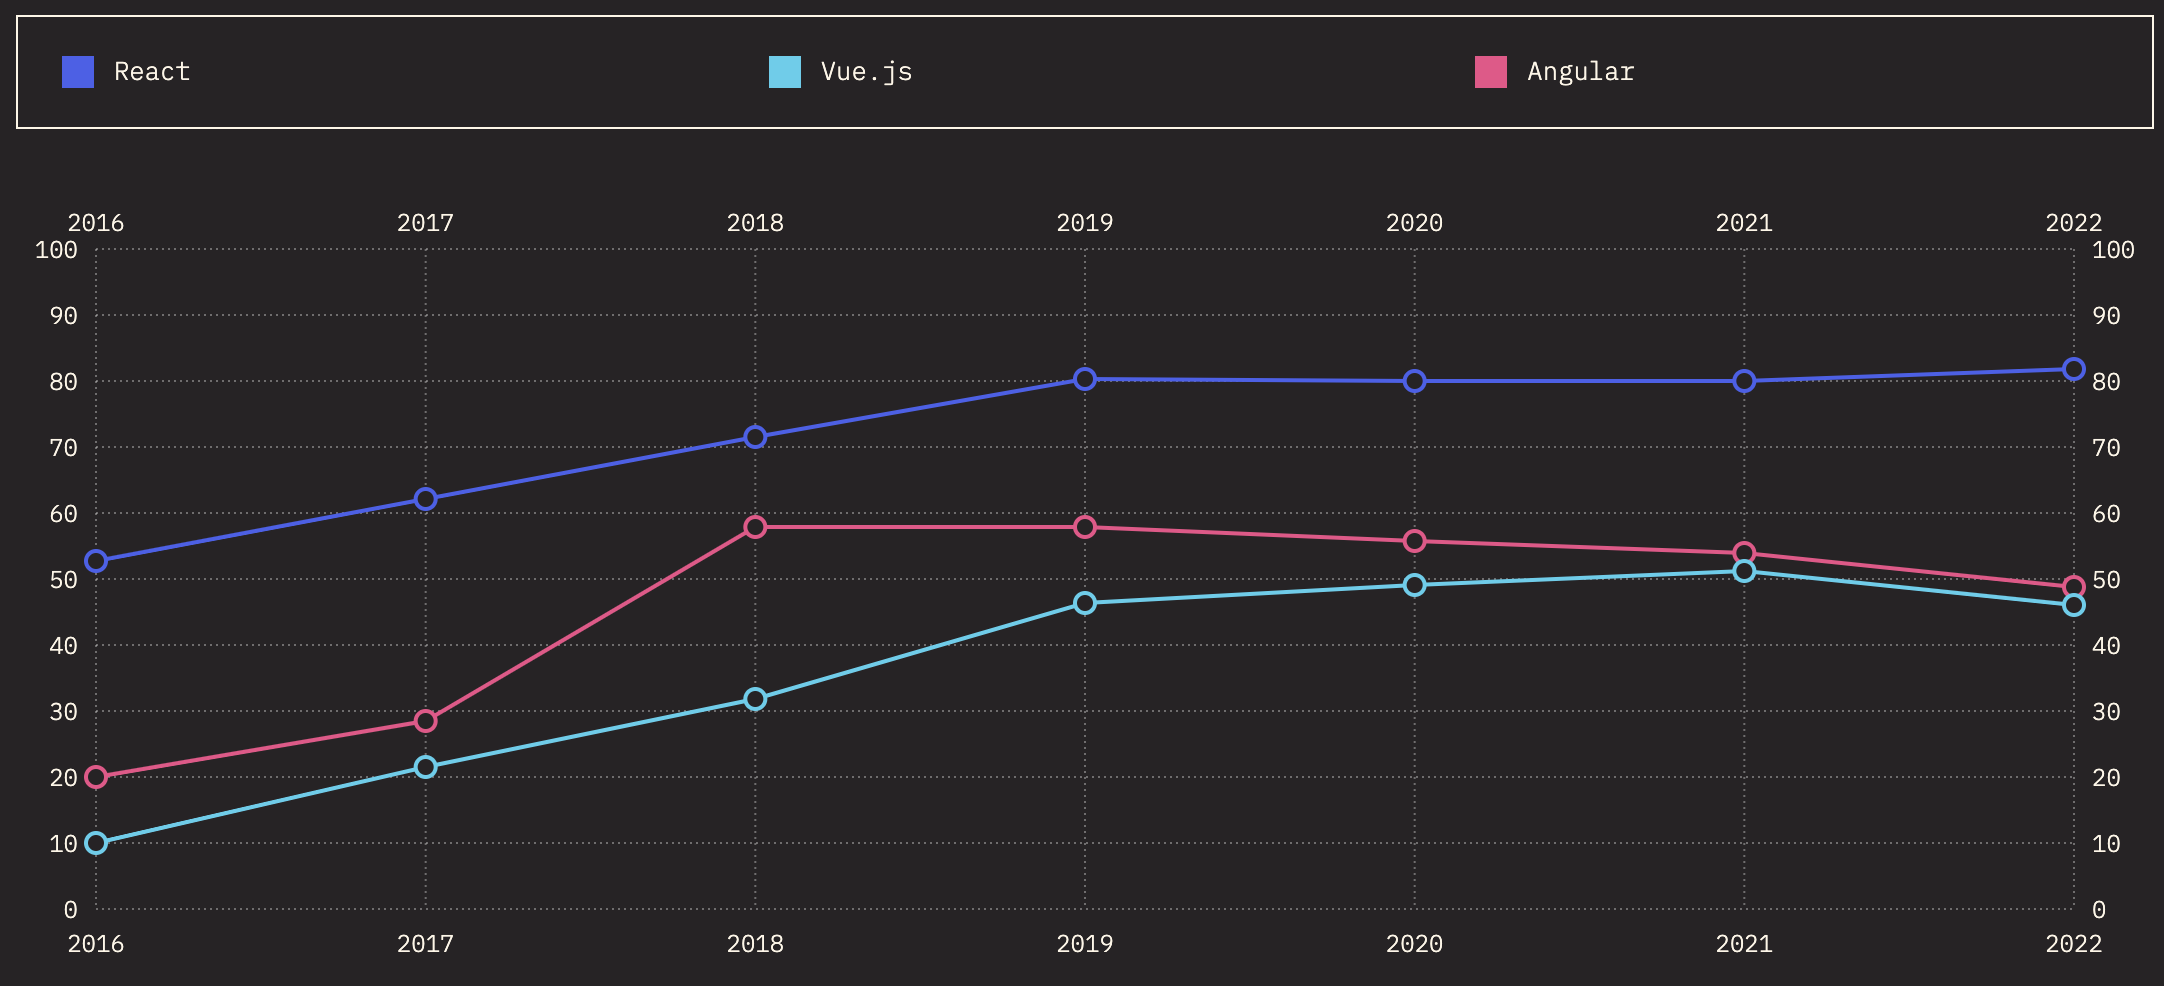
\includegraphics[width=13cm]{dissertation/images/framework_popularity_comparison.png}
    \caption{JavaScript framework/library usage comparison statistics between React, Vue and Angular from 2016 to 2022 from stateofjs}
    \label{fig:js_framework_lib_comp}
\end{figure}

\subsection{Husky}
\href{https://typicode.github.io/husky/#/}{Husky} is an open-source package which allows for easy control over git hooks within JavaScript projects. Husky allows for a developer to run commands on specific \href{https://git-scm.com/docs/githooks}{git hooks} such as \textit{pre-commit} and \textit{pre-commit-merge}. The addition of husky to a project allows for actions such as code testing and linting, presenting a solution to developers forgetting to perform these tasks before pushing code through the pipeline. Husky provides an ecosystem full of plugins and packages that can be used to improve the development of JavaScript packages.

\subsection{Standard Version}
\href{https://github.com/conventional-changelog/standard-version#readme}{Standard Version} is a package which allows for the automatic versioning of a project or packages alongside the automatic generation of a change-log based on commit messages. When used in tandem with Husky Standard Version provides a platform which eliminates the need for developers to manually perform package versioning or the difficult task of ensuring a change log is always up to date.

\section{CLI tool}

The CLI tool takes a different approach in development to the NPM packages as there is a requirement to be run through the command line.

\subsection{NPX }
\href{https://docs.npmjs.com/cli/v7/commands/npx}{NPX} is a command line package runner allowing for the execution of node-based JavaScript packages through a specified command. This has avid usage within the javascript development scene for building starting point directories, popular examples include React's \href{https://reactjs.org/docs/create-a-new-react-app.html}{create-react-app} and Vue's \href{https://cli.vuejs.org/}{vue-cli} to name a few.

\section{Peer}

Integrating a peer-to-peer connection without utilising a self-built and hosted back-end system presented a problem.

\subsection{peerJS}
\href{https://peerjs.com/}{PeerJS} provides an all-in-one solution which utilises WebRTC removing the issue of building a homemade WebSocket back-end system to allow for real-time communication between devices this approach allows developers to keep the simplicity of hosting static files without having to worry about the maintenance and cost of hosting of a back-end system.

\subsection{qrcode Package }
\text Building a bespoke QR code generator did not make sense for this project due to time constraints; to bypass this issue a pre-built solution \href{https://github.com/soldair/node-qrcode#readme}{qrcode} was used. qrcode provides a lightweight solution to building SVG QR codes easily embeddable into a web page. The package converts any given text into a scannable QR code including but not limited to urls and phone numbers. 

\section{Documentation }

\subsection{Docusaurus}
\href{https://docusaurus.io/}{Docusarus} is a documentation generator that takes inspiration from React to provide a platform for easily building and maintaining documentation websites. Developed by Facebook, it is a widely adopted solution for creating high-performing and highly customisable documentation sites thanks to its \href{https://mdxjs.com/}{MDX} support. MDX similar to \href{https://reactjs.org/docs/introducing-jsx.html}{JSX} used within React is a file format which allows the inclusion of componentised JSX within markdown allowing for consistent design with reduced development time. Additionally, Docusarus by default allows for \href{https://www.algolia.com/}{algolia} search integration, an option which adds a full site search to the static site to allow for site-wide searching functionality without the overhead of a backend system to support it. When comparing Docusaurus to the competition, other documentation generators such as \href{https://jekyllrb.com/}{jekyll} and \href{https://www.sphinx-doc.org/en/master/}{sphinx} Docusaurus despite being the newest competitor of the bunch has a wide community and dramatically increases the customizability and performance when compared to the others resulting in documentation sites that arent which can be better custom fit to the projects overall branding and style.


\section{Transpiler}

Building a transpiler is a difficult task to do well, fortunately, there are many packages which can help with steps throughout the processes of parsing, tokenising and code generation allowing for more focus to be put on what needs to be changed. Through Transpiler and its Advantages \cite{kulkarni2015transpiler} the required tools for the development of the transpiler were established.

\subsection{Esprima}
\href{https://esprima.org/}{Esprima} is a JavaScript parser written in JavaScript with the aim of simplifying parsing given ECMAScript 2016 code. Esprima provides functionality for the developer to tokenise and parse JavaScript code into an Abstract Syntax Tree (AST) to the Mozilla (\href{https://developer.mozilla.org/en-US/}{MDN}) JavaScript specification. By providing a comprehensive documentation site Esprima is able to take the hassle out of creating a parser for JavaScript allowing developers to not have to reinvent the wheel and instead put focus on altering the syntax trees to implement their syntax extensions/alterations. 

\subsection{EsCodeGen }
\href{https://github.com/estools/escodegen#readme}{EsCodeGen} is a code generator built for JavaScript which has the sole purpose of converting Mozilla (MDN) compatible Abstract Syntax Trees (ASTs) into readable JavaScript code. EsCodeGen has support for ECMAScript 2016 making it directly compatible with Esprima. This package was utilised due to Esprima's lack of a code generator and avoids the requirement of building a crude module to generate code from the generated ASTs.

%==================================================================================================================================
\chapter{Implementation}

\text Through the analysis of the project's specification a decision was made to separate functionality that is unrelated or can be used independently into their own packages or web applications. This approach resulted in the development of the following packages and web applications shown in figures \ref{fig:packages} and \ref{fig:webapps}.

\begin{figure}[!ht]
    
\begin{center}
\begin{tabular}{|p{2.25cm}|p{5.25cm}|p{5.25cm}|}
 \hline
 \multicolumn{3}{|c|}{Packages} \\
 \hline
 Name  & GitHub repository& Documentation\\
 \hline
Core & \href{https://github.com/espruino-tools/core}{espruino-tools/core}  & \href{https://documentation-xi-liard.vercel.app/docs/category/core}{docs/category/core}  \\

UART & \href{https://github.com/espruino-tools/uart}{espruino-tools/uart}  & \href{https://documentation-xi-liard.vercel.app/docs/category/uart}{docs/category/uart}  \\

Peer & \href{https://github.com/espruino-tools/peer}{espruino-tools/peer}  & \href{https://documentation-xi-liard.vercel.app/docs/category/peer}{docs/category/peer}  \\

Transpiler & \href{https://github.com/espruino-tools/transpiler}{espruino-tools/transpiler}  & \href{https://documentation-xi-liard.vercel.app/docs/category/transpiler}{docs/category/transpiler}  \\

CLI Tool &  \href{https://github.com/espruino-tools/create-espruino-app}{espruino-tools/create-espruino-app}  & \href{https://documentation-xi-liard.vercel.app/docs/category/create-espruino-app}{docs/category/create-espruino-app}  \\
 \hline
\end{tabular}
\end{center} 
    \caption{Table showcasing each package within the ecosystem alongside their respective GitHub repositories and Documentation pages.}
    \label{fig:packages}
\end{figure}

\begin{figure}[!ht]
\begin{center}
\begin{tabular}{|p{2.25cm}|p{5.25cm}|p{5.25cm}|}
\hline
\multicolumn{3}{|c|}{Web Apps} \\
 \hline
 Name & GitHub repository & Site Link\\
 \hline
Online IDE & \href{https://github.com/espruino-tools/online-environment}{espruino-tools/online-environment} & \href{https://online-environment.vercel.app/}{online-environment.vercel.app} \\
Demo's Hub & \href{https://github.com/espruino-tools/demos}{espruino-tools/demos}  & \href{https://demos-mu.vercel.app/}{demos-mu.vercel.app} \\
Documentation & \href{https://github.com/espruino-tools/documentation}{espruino-tools/documentation} & \href{https://documentation-xi-liard.vercel.app/}{documentation-xi-liard.vercel.app} \\
 \hline
\end{tabular}
\end{center}
\caption{Table showcasing each Web App alongside their respective GitHub repositories and hosted site URLs.}
\label{fig:webapps}
\end{figure}

Each of the packages has a unique dependency on each other; this choice of structure allows users to get involved at any step and even develop their own solutions to improve their own custom workflow; the dependency graph is shown in figure \ref{fig:package_dep_graph}


\begin{figure}[!ht]
    \centering
    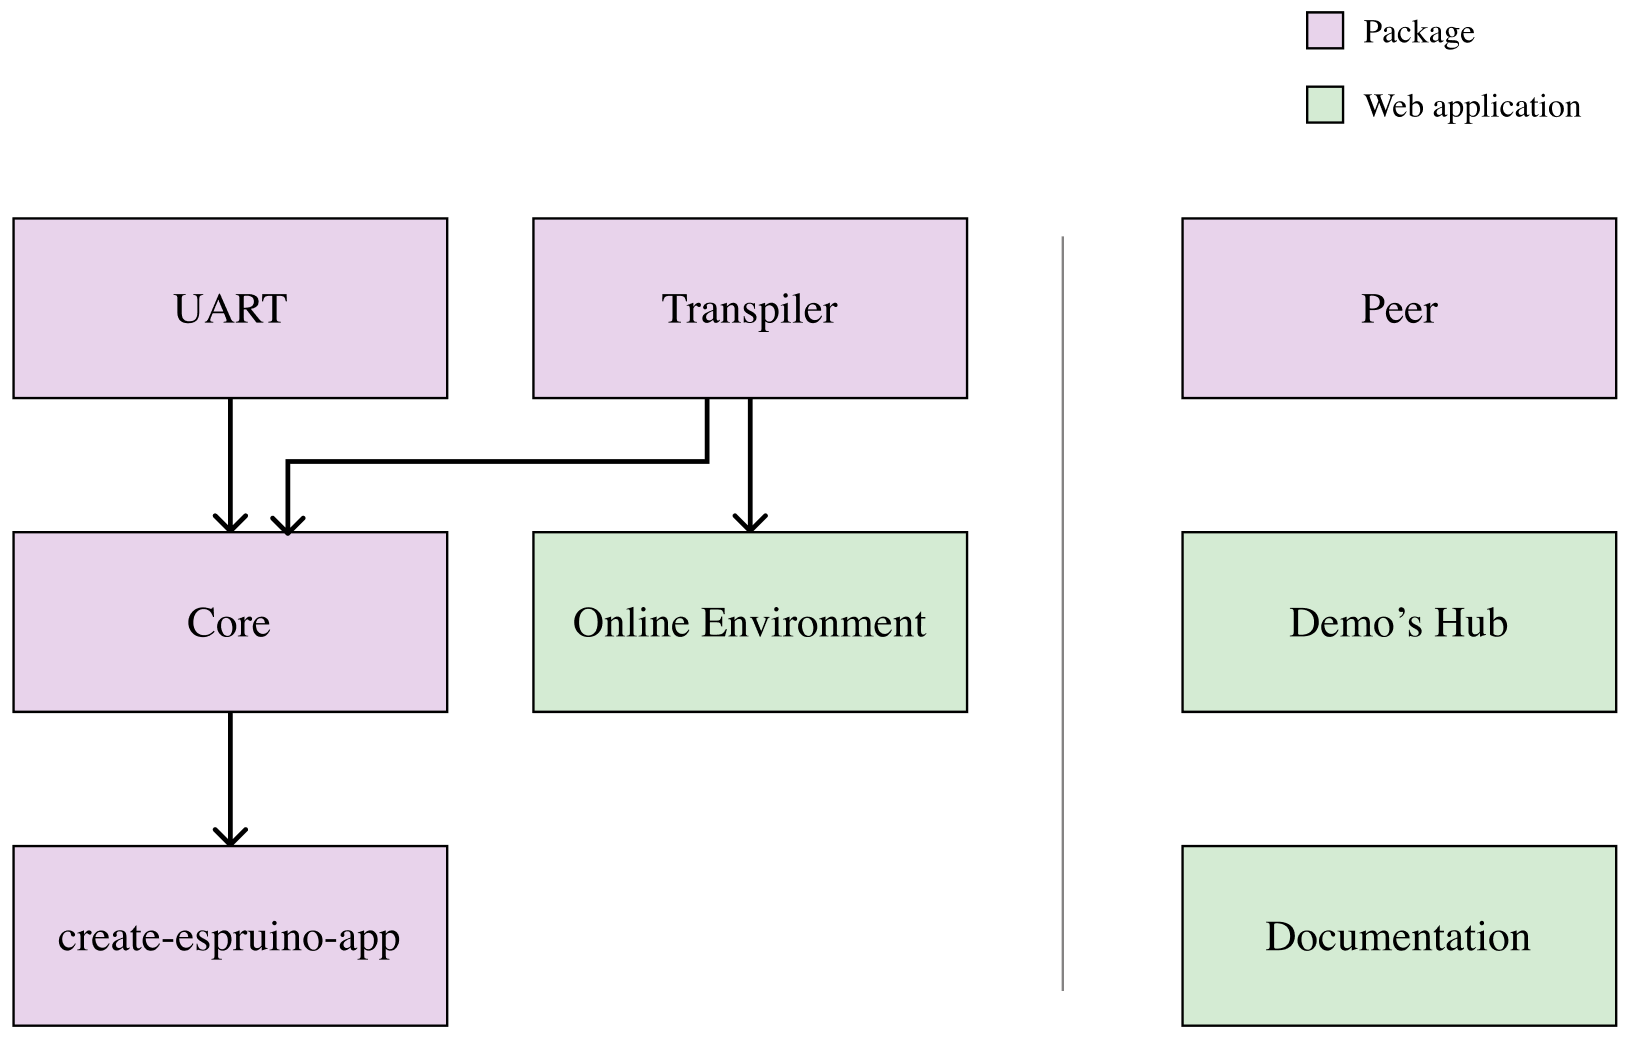
\includegraphics[width=12cm]{dissertation/images/Package_dependency_graph.jpeg}
    \caption{Dependency Graph of the package ecosystem showcasing package dependencies from left to right; Core is dependent on UART and Transpiler, create-espruino-app is dependent on Core and partially Peer if the --peer flag is utilised, Online environment is dependent on the Transpiler package. All other packages have no other dependencies within the package ecosystem.}
    \label{fig:package_dep_graph}
\end{figure}

The packages and web applications above serve as a general view of the ecosystem's structure. The following will showcase the functionality of the packages/web applications in more detail.

\section{Packages}

To provide the end developers with the best possible development, an approach was taken in line with the UNIX ideology \cite{TheArtOfUNIXProgramming} in which functionality is split into their independent parts, maintaining small packages that are functional on their own but can come together to create a more complex project. In addition to this in line with \cite{de2003package} each package is design with the aim to reduce development time and make the process of development as easy as possible.

\subsection{UART}

The UART package is built to enable an easy connection between WebBluetooth/Web Serial devices (such as Espruino devices) and web browsers avoiding the requirement for users to build their own rudimentary solutions. The idea behind the UART package is to improve upon the \href{https://www.espruino.com/UART.js}{uart.js} package. 
\\ \\
uart.js is a library built by the creator of the Espruino platform with the goal of simplifying the interaction between WebBluetooth and Web Serial devices with a web browser. This small package provides users with a means to connect Espruino devices to a browser, but this is all it does leaving no room for user configuration by the developer as well as using old JavaScript methodologies. This approach has resulted in a package which restricts user understanding through a cryptic code base, forces users into incorporating an outdated design into their package in the way of a modal and results in a product that feels unfinished.
\\ \\
The development of the UART package resulted in a package which encapsulated the required functionality of the uart.js package whilst improving in the following aspects: 
\\  
\subsubsection{Modern ECMAScript}\hfill\\
Modern ECMAScript was utilised in the rebuild allowing for a class structure to be used; this approach allows for the end developer to take the core functionality of the package and expand upon it to allow the creation of custom UART implementations, improving the life span of the package whilst not restricting users to using a package which does not offer what they need in their system. By further utilising modern ECMAScript in the development process, the end product produced had a clear direction removing any prior need for global variables or hacky methods of enforcing functionality whilst removing redundant code or code depreciated since the original development of the uart.js package.
\\
\subsubsection{Extension of Functionality}\hfill\\
The original package lacked the functionality to check and alter the queue as well as what commands had previously been sent; this functionality, when used by more experienced developers, would allow for further optimisation during the development of a project with this package resulting in further customisation to fully optimise the end product a goal which is paramount in the development of remote embedded devices.
\\ 
\subsubsection{Improved UI/UX}\hfill\\
By utilising a proper design process, a new non-intrusive modal was developed to improve integration into a more modern style of website whilst enhancing users' experience by incorporating a close modal button omitted in the original package.

\subsection{core}
\begin{center}
\textit{A demonstration of the Core package functionality can be found \href{https://demos-mu.vercel.app/demo/light-sensor}{here}.}
\end{center}
\\
The core package is the ecosystem's main package, which expands upon the UART package by providing users with an experience akin to standard programming. It does this by bypassing issues that occur with sending data to the device; the UART package makes it so that sending code to a device requires the code to be in sting format, leaving the developer in a position where they receive no support from their IDE such as auto-complete suggestions or syntax error detection. The core package provides an importable object for each of the primary Espruino devices as well as an extendable standard import in which users can build their own devices with basic functionality such as connection writing and shared functionality already incorporated. Furthermore, the package provides a more descriptive syntax for the developer, clearing up any confusion or barely documented code. This new syntax, compared with the old, can be seen in \ref{fig:code_approach}.

\begin{figure}[!ht]
\centering
\begin{minipage}{6cm}
  \centering
  \begin{lstlisting}
    let code = `setWatch(function () {
        LED1.toggle();
    }, BTN, {
        edge: 'rising',
        repeat: true,
        debounce: 50
    });`;

    UART.write(code);
  \end{lstlisting}
\end{minipage}
\hspace{1cm}
\begin{minipage}{6cm}
  \centering
  
  \begin{lstlisting}
let p = new Puck()

p.onPress(function(){
    p.LED.toggle('red')
})
  \end{lstlisting}
\end{minipage}
  \caption{Code approach to adding an on-button press event turning on a red LED. This is shown through the current UART.js approach on the Left and through the proposed new "Core" package approach on the right, showing the simplified syntax and removed requirement to write code inside a string.}
  \label{fig:code_approach}
\end{figure}

On top of this, the core package takes a fully asynchronous approach to development, taking advantage of JavaScript's \textbf{Promise} functionality utilising \textbf{async/await}. This allows the developer to not worry about using timeouts throughout their program but instead opt for a cleaner solution that presents data when it's ready instead of when a hard-coded timer has passed. This is baked-in functionality meaning the \textbf{async/await} keywords can be utilised to gather data from the device, as shown below in figure \ref{fig:async-await-core}.

\begin{figure}[!ht]
    \centering
    \begin{lstlisting}
let p = new Puck();

let temperature = await p.getTemperature();
    \end{lstlisting}
    \caption{Proposed solution to removing the requirement for set length timeouts through the utilisation of JavaScript's Promise feature, specifically the async/await functionality}
    \label{fig:async-await-core}
\end{figure}

\textit{We can see in the figure }\ref{fig:async-await-core} \textit{a top-level await is utilised, due to the usage of modern JavaScript throughout the package ecosystem, this option is available.}

\subsection{Peer}
\begin{center}
\textit{A demonstration of the Peer package functionality can be found \href{https://demos-mu.vercel.app/demo/pixl-dinosaur-demo}{here}.}
\end{center}
\\
\text Involving peer-to-peer connection within the package ecosystem required the addition of a WebRTC-compatible package. To solve this problem, the Peer package was built as an extension to the peer.js platform. peer.js is an open-source package that provides functionality to facilitate the peer-to-peer connection between two browsers. 
\\ \\
The Peer package extends upon the functionality of peer.js by adding some ease of life functionality, such as simplified connection via a modal that combines a scannable QR code alongside a link which redirects to a page via query string. This can be seen in figure \ref{fig:qr-scan}. 
\\ \\
\begin{figure}[!ht]
    \centering
    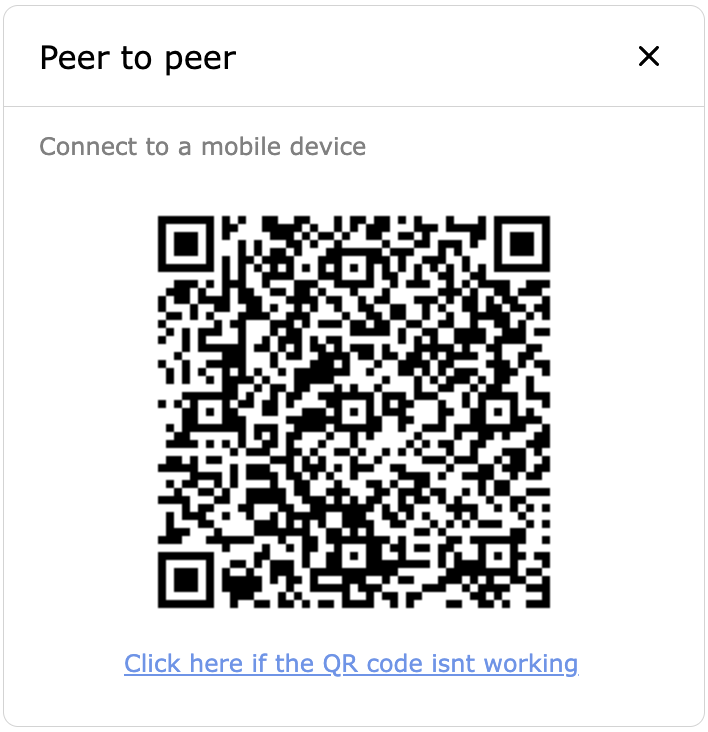
\includegraphics[width=6cm]{dissertation/images/QR-p2p-modal.png}
    \caption{Design snippet for the Peer packages connection modal utilising a QR code for easy mobile connection through camera scanning.}
    \label{fig:qr-scan}
\end{figure}

\text In addition to this the Peer package implements a simplified syntax for setting up data and video transmission between two browsers, this syntax can be seen below in figure \ref{fig:peer-syntax} showing basic data connection.

\begin{figure}[!ht]
\centering
\begin{minipage}{7cm}
  \centering
  \begin{lstlisting}
// Hosting page
let p_host = new Peer();
p_host.on('connection', (conn) => {
  conn.on('data', (data) => {
    console.log(data)
  });
});

// Connecting page
let p_connector = new Peer();
let conn = p_connector.connect(peer_host.id);
conn.on('open', () => {
  conn.send('my message');
});
  \end{lstlisting}
\end{minipage}
\hspace{1cm}
\begin{minipage}{5.5cm}
  \centering
  
  \begin{lstlisting}
// Hosting page
let p_host = new Host();
p_host.getData(data => {
    console.log(data);
});
 

// Connecting page
let p_connector = new Connector();
p_connector.connectData();
p_connector.conn
    .send("my message");

  \end{lstlisting}

\end{minipage}
  \caption{Code approach to initialising a simple peer-to-peer connection through a hosting page and connecting page approach with peer.js (Left) and the new Peer package (Right) showing the simplified and more readable syntax used in the Peer package approach (Left)}
  \label{fig:peer-syntax}
\end{figure}

The examples above glosses over how the hosting site passes the id across, within the peer.js package, a bespoke approach to this would be required, whereas the Peer package will do this by default, further removing another step of boilerplate configuration from the developer


\subsection{create-espruino-app}
\begin{center}
    
\textit{A demonstration of the CLI Tool's functionality can be found \href{https://demos-mu.vercel.app/demo/create-espruino-app}{here}.}
\end{center}
\\
To ensure users can get started with Espruino-tools as soon as possible and with as little setup as possible, the create-espruino-app package presents a CLI tool to allow the construction of a customised directory ready to start development with a single terminal command. The package will clone a specified git repository based on the provided flags and will provide a repository with a customised Webpack configuration that allows for localhost development alongside an easy build command to allow projects to be hosted directly on GitHub pages for easy project sharing. Below in figure \ref{fig:flag-comp} shows a table of flags available to the user alongside what they produce.

\begin{figure}[!ht]
    \centering
    \begin{tabular}{|p{2.25cm}|p{10cm}|}
 \hline
 \multicolumn{2}{|c|}{Flags} \\
 \hline
 \textbf{Flag}  & \textbf{Use case}\\
 \hline
 template & This flag allows for users to specify the environment they want to get started with this includes plain JavaScript, TypeScript, React and Vue.\\ \hline

 peer & Allows for an environment using the Peer package with two pages to be set up one for the Host page and one for the Connector page, this takes each template's routing systems into account and provides a routing system for those that do not have one.\\ \hline

 clean-install & This allows users to get started with an environment from the template tag with no additional setup, this will just provide an empty page and the correct packages installed to allow full control over what the project does without guidance from the tool.\\
 \hline
    \end{tabular}
    \caption{A table showcasing the array of flags supported by the CLI tool allowing features such as; flexible environments through the --template tag supporting React, Vue, Typescript and standard Javascript, easy peer package setup through the --peer syntax as well as a simplified work environment for more experienced developers through the --clean-install flag.}
    \label{fig:flag-comp}
\end{figure}

This tool works through NPX, meaning that users are not required to install anything to utilise the tool. This choice was made to make the usage of the tool as accessible as possible to a wide audience of developers. An example of a command used to produce a React and Peer-enabled package in a directory called \textit{my-esp-app} is shown below in figure \ref{fig:npx-command}.

\begin{figure}[!ht]
    \centering
    \begin{lstlisting}[language=bash]
        $ npx create-espruino-app my-esp-app --template react --peer
    \end{lstlisting}
    \caption{Example command line input for an espruino-tools project with a react environment that supports the Peer package out of the box. This utilises the --template and --peer tags to achieve this.}
    \label{fig:npx-command}
\end{figure}

\subsection{Transpiler}
\begin{center}
\textit{A demonstration of the Transpiler package functionality can be found \href{https://demos-mu.vercel.app/demo/transpiler}{here}.} 
\end{center}
\\
As the development of the core package progressed, it became apparent that the previous implementation of converting the new syntax of code into espruino natively compatible code was not covering the code adequately and was resulting in basic features such as variable declaration or any statements with a scope not translating correctly. To counter this problem, the Transpiler package was created; the Transpiler package provides a platform for converting code in the espruino-tools syntax into native espruino code. The package utilises Esprima and escodegen, tools that convert code into abstract syntax trees (ASTs) and back, allowing the package to focus on transforming the ASTs for syntax conversions.
\\ \\
Due to the approach of constructing, transforming and building ASTs the Transpiler package creates a tool which only converts code recognised to be espruino-tools code leaving the rest to remain as standard JavaScript; this approach further allows users to incorporate native Espruino code into their projects meaning new features within the standard ecosystem are not restricted when using the espruino-tools ecosystem of packages.
\\ \\ 
An example of the input and output of the Transpiler package can be seen below in figure \ref{fig:transpiler-input-output}.

\begin{figure}[!ht]
\centering
\begin{minipage}{6cm}
  \centering
  \begin{lstlisting}[
    basicstyle=\footnotesize
]
let p = new Puck();
p.mag.onMag(val => {
    if(val > 2){
        p.LED.on("blue");
    } else {
        p.LED.off("blue");
    }
})

  \end{lstlisting}
\end{minipage}
\hspace{0.5cm}
\begin{minipage}{6cm}
  \centering
  
  \begin{lstlisting}[
    basicstyle=\footnotesize
]
Puck.on('mag', function (val) {
    if (val > 2) {
        LED3.set();
    } else {
        LED3.reset();
    }
});
  \end{lstlisting}
\end{minipage}


  \caption{Process of the transpiler package showing the input on the Left and the output on the right. This shows the simplified and more readable syntax from the espruino-tools syntax (Left) generated into the standard Espruino output required to run on the Espruino devices (Right)}
  \label{fig:transpiler-input-output}

\end{figure}

\section{Web Apps}
To provide developers with a complete ecosystem, web applications were also developed to provide a community for sharing projects as well as a platform to test the functionality of code on devices quickly.

\subsection{Online environment}
\begin{center}
\textit{The online environment can be visited \href{https://online-environment.vercel.app/}{here}} 
\end{center}
\\
\text The online environment provides a platform for users to develop their Espruino devices from a browser whilst having a terminal output to allow a more in-depth dive into bug diagnostics.
\\ \\
The online environment provides users with the functionality to quickly perform actions on Espruino devices. The platform can be used fully within the development of Espruino packages allowing users to upload code to the editor as well as download their code into a JavaScript file. Users can use the platform to connect and run code directly on the device, reset the device or gather both functions on the device alongside the code on the device itself this can be seen in figure \ref{fig:online-env-device-code}

\begin{figure}[!ht]
    \centering
    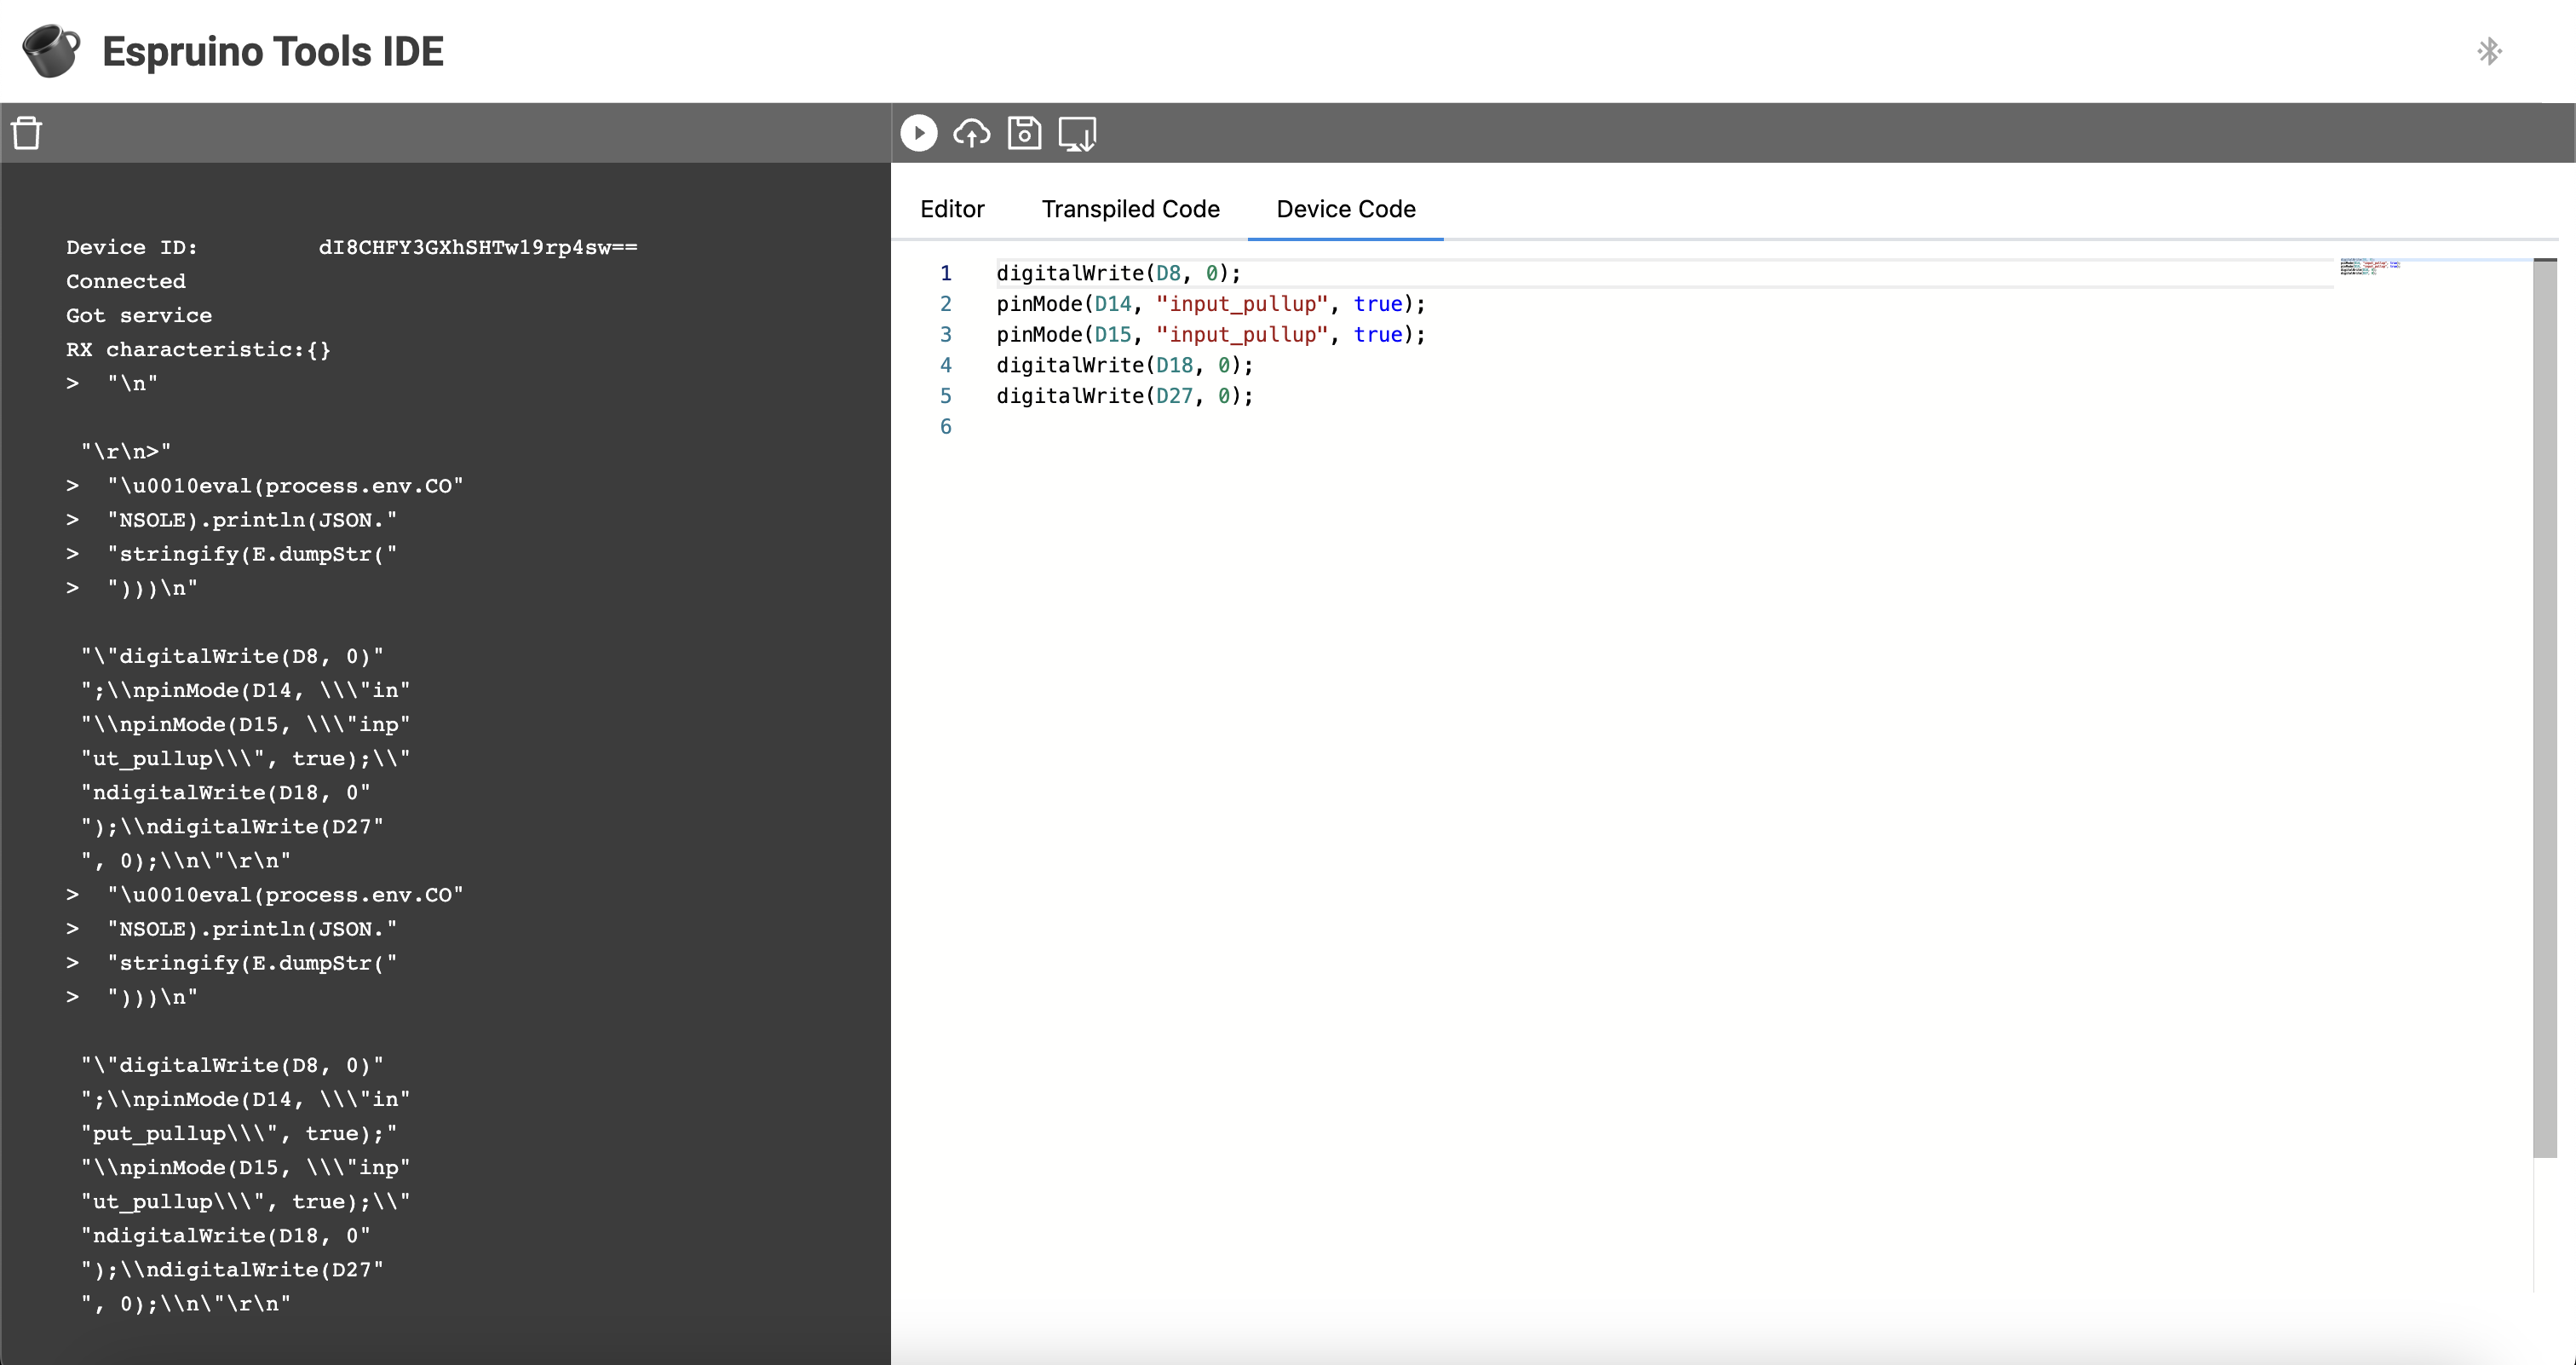
\includegraphics[width=11cm]{dissertation/images/online-env-device-code.png}
    \caption{The developed Online environment showcasing the terminal output (on the left) side by side with the code stored on the device (on the right). This added feature improved the debugging ability of developers and presents an improvement over the original Espruino IDE.}
    \label{fig:online-env-device-code}
\end{figure}

Alongside this feature the web application provides the ability to view transpiled code, this could be used to gain the benefits of the clean concise espruino-tools code without using the packages themselves allowing for flexibility in the users' development style.
\\
The environment utilises the Monaco editor, a code editor for web applications built by Microsoft to replicate the vs code editor, this choice was taken to keep the environment as similar as possible for the developer.

\subsection{Demo's Hub}
\begin{center}
\textit{The demo hub can be visited \href{https://demos-mu.vercel.app/}{here}} 
\end{center}
\\
To provide a platform for users to view what can be built with espruino-tools the Demo's Hub was built. This web application provides a place for new or experienced users to browse projects built with espruino tools including an experience with easy downloading of code as well as a code viewer to browse the code base required to produce the result. The site provides an individual page for each unique project this can be seen in figure \ref{fig:demo-page}.

\begin{figure}[!ht]
    \centering
    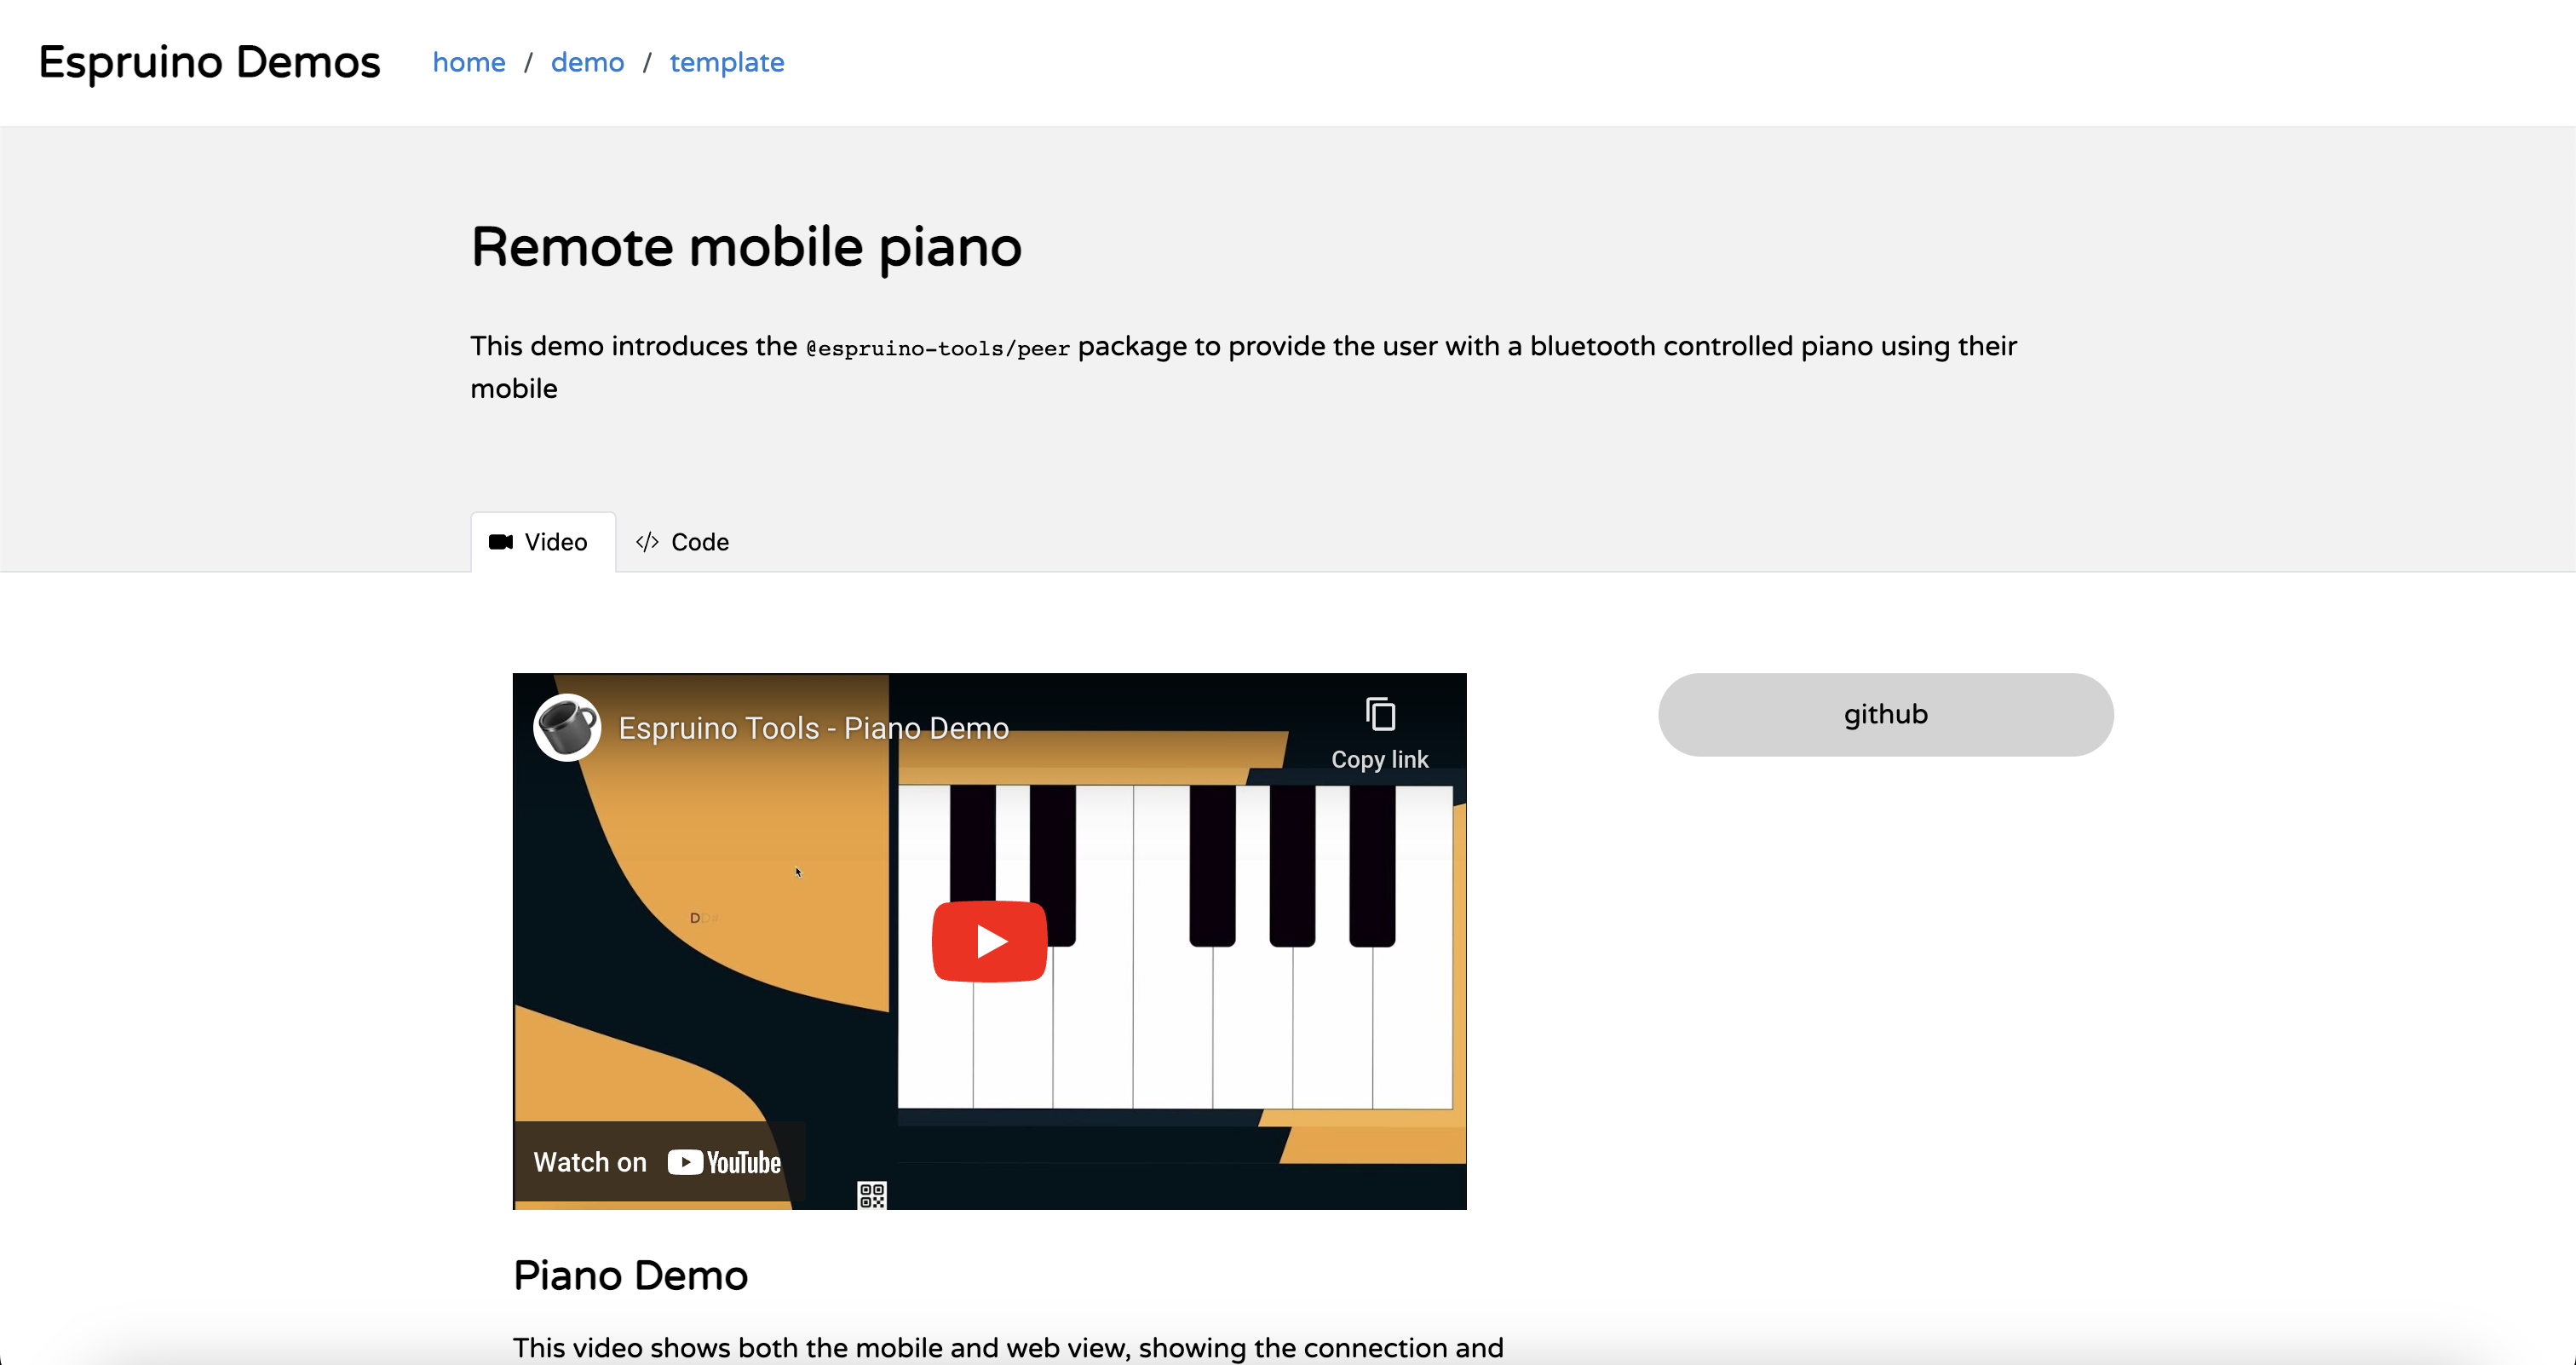
\includegraphics[width=11cm]{dissertation/images/demo-page.png}
    \caption{project page on the demo site showcasing the ability to embed details such as short descriptions and a title alongside a youtube video with again a title and description. Finally allowing for users to enter sidebar links in this case showing the GitHub repository of the project}
    \label{fig:demo-page}
\end{figure}

The page is customised by the developer by utilising the custom espruino demo configuration file, this JSON file allows developers to add videos via youtube's embedded link sharing, descriptions and custom links to fully cover what their page does an example of this JSON configuration file can be seen in the figure \ref{fig:demo-config}

\begin{figure}[H]
    \centering
    \begin{minipage}{10cm}
    \begin{lstlisting}[
    basicstyle=\footnotesize
]
{
    "projectHeader":{
        "title":"Demo title",
        "projectDescription":"demo header description"
    },
    "sidebarLinks":[
        {"name":"github","link":"https://github.com/"},
        {"name":"optional custom link","link":"https://..."}
    ],
    "video":{
        "link":"https://www.youtube.com/embed/z0YW8AEI8LM",
        "details":{
            "title":"Video title",
            "description":"video description"
        }
    }
}
    \end{lstlisting}
    \end{minipage}
    \caption{Code overview of an example demo configuration file that specifies project details with a youtube video and two sidebar links.}
    \label{fig:demo-config}
\end{figure}


To allow users to add their own contributions without building and hosting a dedicated backend system due to time constraints, the demos hub is populated through the GitHub repositories \textit{demos} folder. This approach means that developers have to create a pull request within the demos repository adding their project, with clear instructions on the demo's hub site; this approach provides the benefits of a backend system not requiring the site to be rebuilt on an added change whilst bringing the benefits of a statically generated site not requiring any cost to host online.

\section{Documentation}
\begin{center}
\textit{The documentation site can be visited \href{https://documentation-xi-liard.vercel.app/}{here}} 
\end{center}
\\
\text Due to the package ecosystem incorporating many different concepts and packages, a documentation site was required to help provide a place for all documentation in one well-organised place. The implementation of the documentation produced a platform where users can search for concepts within any package available whilst being presented with tutorials on using the technologies and videos showcasing the products produced. The development of the documentation heavily utilised components for consistent styling, meaning that pages are based on a preset custom template which provides options for code editors, sandboxed environments as well as video implementation with little to no boilerplate code meaning new features can be added to the documentation with little to no effort ensuring an up to date and accurate documentation site can be easily maintained.

\section{CI/CD}
The CI/CD pipeline built provides a platform that streamlines the development process of the packages; this process provides the structure for how the packages are tested and prepared before deployment alongside how they are deployed, leaving the focus on the programming and less on the semantics of deploying an application \cite{CICD}. To allow the CI/CD pipeline to effectively have stages for each process to be run an effective branching structure was required to be built, through the branching structure shown in \cite{FeatureBranching} this was able to be achieved through effectively named and protected branches. This is shown below in Figure \ref{fig:CICDPipeline}  

\begin{figure}[!ht]
    \begin{center}
        
    
    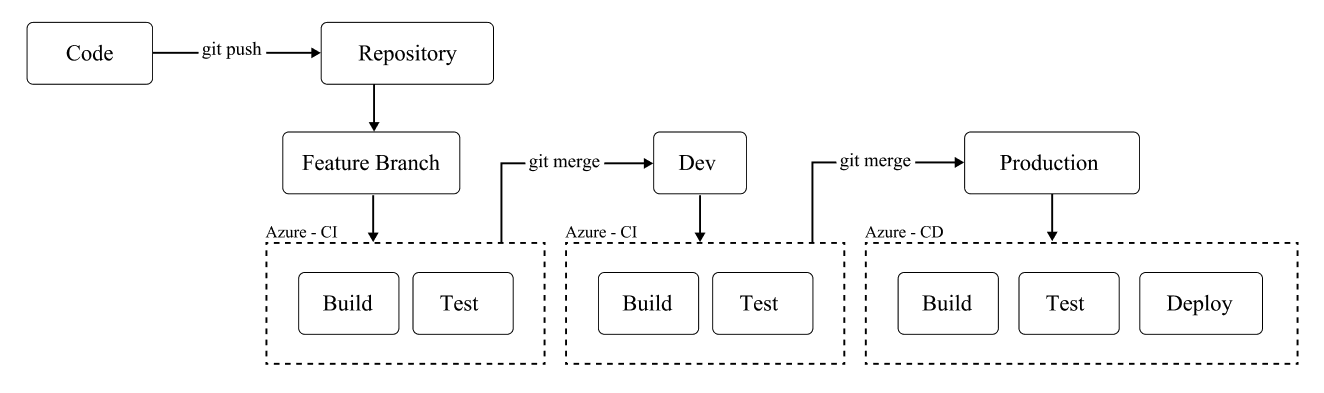
\includegraphics[width=12cm]{dissertation/images/CICD-structure.png}
    \end{center}
    \caption{CI/CD Pipeline flow from code to deployment including the branching structure and build and test process throughout.}
    \label{fig:CICDPipeline}
\end{figure}

Implementing this branching structure for the CI/CD before the projects had begun ensured that only functional changes were published to NPM, meaning no broken packages were able to make it through the pipeline due to the journey required to reach deployment.

\section{Deployment}
To ensure the packages and web applications are widely available to any potential developers a proper approach to deployment had to be taken ensuring both reliability and low to no cost.

\subsection{Packages}
% UNFINISHED
The deployment of packages was facilitated through the usage of an azure pipeline. This process when combined with the effective CI/CD described above allowed for a streamlined process.
\\ 
As the packages needed to be served by both NPM and UNPKG both a built version and a minified built version were required to be created to achieve this a Webpack script was produced to allow for the pipeline to build both required configurations; this process would also convert the TypeScript library into JavaScript. We can see the process of the pipeline in figure \ref{fig:deployment}

\begin{figure}[H]
    \begin{center}
    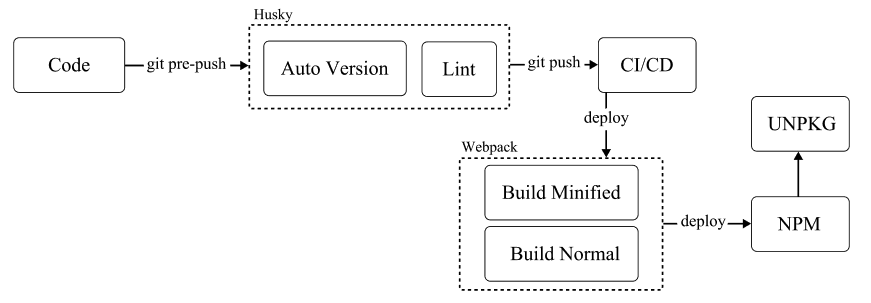
\includegraphics[width=12cm]{dissertation/images/Deployment.png}
    \end{center}
    \caption{Package deployment flow graph from code to deployment including package versioning through Husky and multiple build outputs through Webpack.}
    \label{fig:deployment}
\end{figure}

The process utilises NPM's publish command which utilises the version of the package within the packages configuration files to create a new version of the package in NPM's package database; this is facilitated with the help of husky and standard version to automatically increment the version on changes pushed. A benefit of utilising standard version is the automatic creation of a changelog which is highly beneficial for the package ecosystem. As for UNPKG when an NPM package is published UNPKG will automatically create a link which can be used to gather the package this allows for no requirements to host the package on a CDN reducing costs to nil.

\subsection{Web Apps}
% UNFINISHED
A different approach was required to deploy the web applications as the package deployment did not require a standalone server. As React was being used, Vercel was chosen as the optimal approach; Vercel provides its pipeline, which deploys a version of the web application on each branch used, allowing for development site testing before pushing to production. As the React site is built and compressed via gzip, we are left with a static website. Vercel provides a service to freely serve static websites meaning the web applications are hosted at no cost. This process can be seen in figure \ref{fig:web-app-deploy}

\begin{figure}[H]
    \centering
    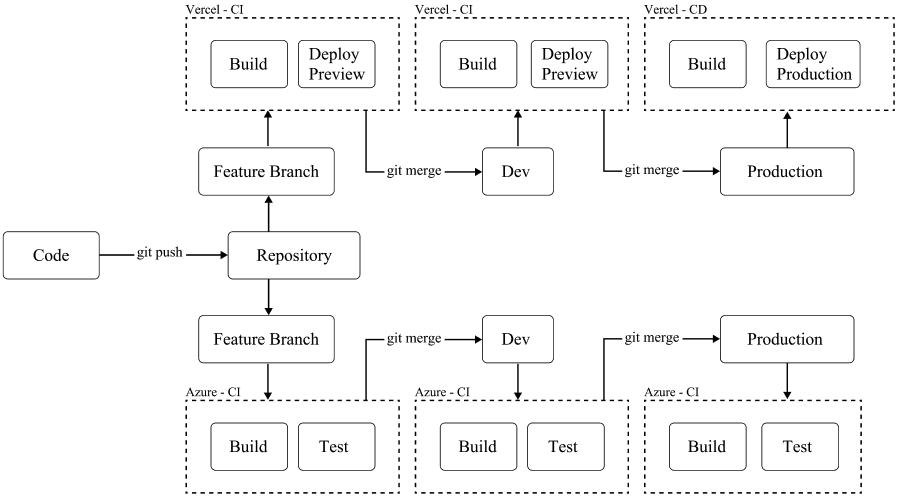
\includegraphics[width=12.5cm]{dissertation/images/web-app-deploy.png}
    \caption{Web application CI/CD flow utilising both azure DevOps and vercels CI/CD pipelines. Vercel provides the ability for preview deployments and production deployments to be built at every stage of the process allowing for better feedback on changes in a production-style environment}
    \label{fig:web-app-deploy}
\end{figure}

\chapter{Evaluation} 

\section{User Feedback}
Throughout the full project, a user study was utilised to receive a constant stream of feedback. The developer used within the study had no prior knowledge of node.js and was tasked in building a project which incorporated every aspect of the package ecosystem; the approach taken to receiving this feedback allowed for a direction of package development which was heavily influenced by an expected heavy use-case of the ecosystem.
\\ \\
The task at hand had the developer develop a self-driving car which utilised an Espruino Pixl device to control motors. This project required camera input, easy control over the Espruino device as well as instantaneous response time from the input. These tasks resulted in specialised feedback in the following areas:

\subsection{Core}
With the core package being the main component in device interaction, this package was heavily utilised within the development of the project. This prompted the following additions to the package

\subsubsection{Code upload}\hfill\\
To allow the developer to quickly and easily incorporate code from a URL device, functionality was added to accommodate this and allow direct running within the device, removing any requirement for the code base to be stored on a device, allowing for easier project sharing.
\subsubsection{Custom device configuration}\hfill\\
As a custom device was being developed on the standard devices Puck, Pixl and Bangle, all incorporated functionality which was not available on newly created devices. To combat this, a core device \textbf{DeviceController} was implemented, which encouraged inheritance to allow for newly developed devices to incorporate basic functionality and expand with device-specific functionality.
\subsection{Peer}
For the self-driving car to be able to follow a track, it is required means to incorporate effective video input. The requirement for this prompted the addition of the Peer package. Following the initial development of this package, the developer's feedback prompted the following additions to the package:

\subsubsection{Simultaneous video and data transfer}\hfill\\
The project required input to be received from both the camera and touch input within the same connection. To allow for a mobile device to both utilise video for tracking as well as touch input to enable control of the system from the car device itself, the package was configured to allow for this multiple inputs to be transferred at the same time.
\subsection{UART}
As the project required instantaneous data transfer between the browser and the device, it became apparent quickly into the development of the project that the original UART rework had not taken into consideration a speed improvement over the original. This revelation prompted a rework of the UART package to remove unnecessary waits and time delays whilst incorporating the modern Promise feature of JavaScript.

\subsection{NPX Tool}
As the developer had not utilised node.js within a project beforehand, the development of the NPX tool had many reiterations to incorporate the following issues raised:
\subsubsection{Serving static assets}
As the tool produced environments utilising Webpack to build and provide a local development server server, there quickly became an issue with incorporating basic static site functionality to developed sites, in this case, including images in the site. To resolve this issue, the repositories were equipped by default with the functionality to include images or other static images into the project to allow transfer into the build folder.
\subsubsection{Peer package incorporation}
For local development, the WebRTC API utilised within the Peer package presented issues for the developer within local development using a mobile device. This issue required the usage of a local IP as well as the integration of false SSL, the feedback from this feature introduced a new method of utilising Webpack to host a local environment for development purposes.
\subsubsection{Deployment}
As the project utilised a local node server for development, the developer was unsure of how this should be deployed as it was a static site; this prompted the addition of Webpack to build the project into a single build folder allowing for deployment on GitHub pages. In addition, further feedback incorporated a simple script to the packages to create a new branch that moves the build folder content into the root level, which can then be hosted on GitHub pages.
\section{Core Package Evaluation}

The core package presents an option built on top of the original Espruino native code syntax to allow users a cleaner and more transparent approach to the same problems whilst bringing in some ease-of-life functionality; for this to be effective, the package needs not to be detrimental to the run time of the code or writing of code to the device.
\\ \\
To ensure the additional features did not negatively affect the performance, a test was created that pits the uart.js package with the core package, ensuring the following criteria were met:

\begin{itemize}
    \item code snippets are the same length (500 characters long).
    \item both packages were set up in a standard working environment without additional features that could slow things down.
    \item each test should be run 25 times to ensure stray figures do not skew the data.
\end{itemize}

The following figure \ref{fig:core_native_speed} shows the results from the 50 total run tests.

\begin{figure}[H]
    \centering
    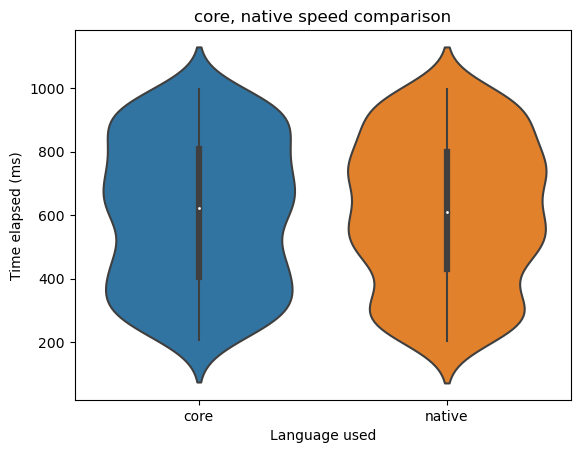
\includegraphics[width=12cm]{dissertation/images/core-native-speed.png}
    \caption{Graphed speed comparison between writing code to an Espruino device through the core package and through the native uart.js package. The results from this showcase that the main bottleneck is with the WebBluetooth API meaning there is not a noticeable performance difference between these packages despite the requirement for the transpiler to be run on the core package}
    \label{fig:core_native_speed}
\end{figure}

The results from the tests run found that despite the requirement for a transpiler to be run first before writing the code to the device the main bottleneck of the data transfer to Espruino devices comes from the WebBluetooth API meaning that despite the additional functionality there are no notable differences in transfer speed spanning from the additional overhead.

\section{Peer Package Evaluation}

For the peer package to be a viable method of introducing new device inputs and outputs across multiple previously incompatible platforms, the package must incorporate seem-less communication between the secondary browser and the Espruino BLE device.
\\ \\
The Peer package brings in a new potential bottleneck by introducing the WebRTC API into the system by utilising another connection-based data transfer, this time through an internet connection instead of a Bluetooth connection. This obstacle means that the data sent from a typical user's mobile device has to be sent to another device than from that device to the Espruino device.
\\ \\ 
To ensure the peer package was not rendered useless by this chain of connections, a test was taken out to check the data transfer speed of both standard data transfer from a compatible browser to an Espruino device as well as the data transfer from a non-compatible device through the Peer package to an Espruino device. For this comparison to be an accurate representation, the following criteria were used to maintain consistency:

\begin{itemize}
    \item code snippets of the same length (250 characters long)
    \item code snippets are both in native Espruino code (avoids transpiling time difference)
    \item test will be run 1000 times to remove any variance due to outlying data.
\end{itemize}

Below in figure \ref{fig:peer-native-speed-comparison}, we can see the results from this experiment.


\begin{figure}[H]
    \centering
    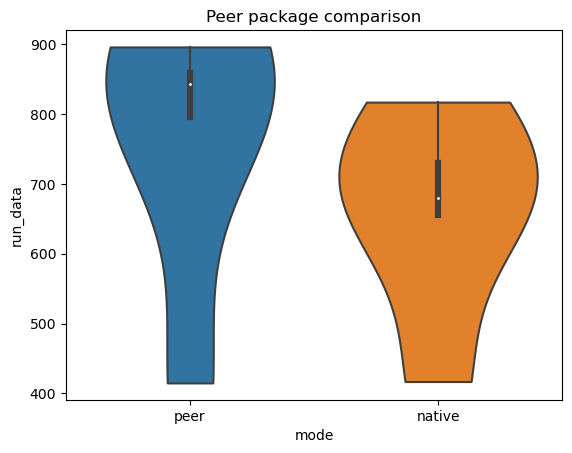
\includegraphics[width=11cm]{dissertation/images/peer-native-comparison.png}
    \caption{Graphed speed comparison between using the Peer package and natively transferring data to the device(without a peer-to-peer connection). This graph showcases how there is not a noticeable average run time between the two options again due to the data transfer through the WebBluetooth API, again making it the bottleneck here.}
    \label{fig:peer-native-speed-comparison}
\end{figure}

From the results in figure \ref{fig:peer-native-speed-comparison}, we can see that the peer and native produce nearly identical results showing that the additional variance due to the Peer package addition creates minimal friction in data transfer, meaning the Peer package is a viable option to incorporate unsupported devices into the Espruino ecosystem.

\section{Transpiler Package Evaluation}

The original development of the miniParser module was prompted due to the requirement for entire segments of code to be converted from espruino-tools syntax into Espruino native code. As this step was impossible through building an object with methods, a small module was required to be created.
\\ \\
The original miniParser was built as a temporary solution to a bigger problem. The miniParser falls short with its ability only to convert single-line statements or un-nested code resulting in the lack of ability to use standard programming conventions such as conditionals, loops or functions within methods that take functions as parameters. 
\\ \\ 
The development of the transpiler package was begun due to these shortcomings. The transpiler takes an approach similar to a traditional compiler converting the code into an AST, transforming it and then generating code from the altered AST.
\\ \\ 
To compare these two approaches, a small set of tests with the code snippets specified in figure \ref{fig:transpiler_code_snippets}.

\begin{figure}[H]
    \centering
    \begin{minipage}{3.5cm}
        \centering
        \begin{lstlisting}
            let p = new Puck();
        
            p.LED.on("red");
        \end{lstlisting}
        Simple
    \end{minipage}
    \hspace{0.5cm}
    \begin{minipage}{3.5cm}
        \centering
    \begin{lstlisting}
      let p = new Puck();
      let light = p.getLightVal();
      light > 0.2 
        ? p.LED.on("red") 
        : p.LED.off("red");
    \end{lstlisting}
    Conditional
    \end{minipage}
    \hspace{0.5cm}
    \begin{minipage}{4.5cm}
        \centering
        \begin{lstlisting}
    let p = new Puck();
    for(let i = 0; i<33; i++){
        if(i % 3 === 0){
            p.LED.toggle("red");
        }
        p.LED.toggle("green");
    }
    \end{lstlisting}
    Nested
    \end{minipage}
    \caption{Code snippets used within the transpiler comparison chosen to cover different aspects of programming from; device initialisation in Simple, Conditional LED setting through lambda statements in Conditional to Simple nested code using a conditional if statement inside of a for loop in Nested.}
    \label{fig:transpiler_code_snippets}
\end{figure}

% \begin{figure}[!ht]
    
%     \caption{Conditional}
%     \label{fig:conditional_transpiler_code}
% \end{figure}

% \begin{figure}[!ht]
%     \centering
    
%     \caption{Nested}
%     \label{fig:nested_transpiler_code}
% \end{figure}

Each code snippet was run 25 times on both the transpiler and miniParser to test the speed of the code converters with increasingly complicated code snippets to compare the code coverage of the package. The following figure \ref{fig:transpiler-miniparser-speed-comparison} shows that despite more complicated code having a longer conversion time in the transpiler, the miniParser fails on all accounts but the simple code snippet.

\begin{figure}[H]
    \centering
    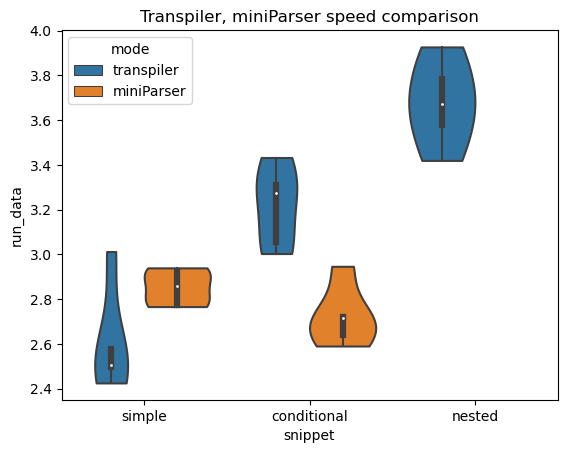
\includegraphics[width=11cm]{dissertation/images/transpiler-miniParser-speed-comparison.png}
    \caption{Graphed results from the Transpiler test showcasing the miniParser having a near consistent run-time whilst the transpiler time increased as the code complexity increased. Despite the shorter run time, the miniParser does not correctly run for the conditional sample and throws an error when running on the nested code sample }
    \label{fig:transpiler-miniparser-speed-comparison}
\end{figure}

The figure shown \ref{fig:transpiler-miniparser-speed-comparison} shows that the miniParser ran without failing two of the three times. Despite this on the conversion for the conditional code snippet, the miniParser could not correctly convert the code snippet. As for the nested code snippet, the miniParser threw an error resulting in no code output.


\section{Testing}
Various testing approaches were taken based on the package or web application type to make the most of the pipeline and ensure the code base was as robust and functional as possible.

\subsection{Unit testing}
% Extend with coverage / what was tested / methods of testing.
A unit testing approach was taken for packages, and JEST was used alongside mocking with JSDOM. This approach allowed for a fake DOM and WebBluetooth to test the package independent from the device connection and the browser actively running. JEST is a standard test runner package that allows a developer to create conditions that need to be met for a package to be considered functional; when combined with Test Driven Development (TDD), this provided an architecture for how the packages were meant to function. JSDOM is a package that mocks standard web browser functionality allowing WebAPI's to be tested without requiring a browser to run.
\\
The unit testing suite covers the following features:
\begin{itemize}
    \item UART device connection.
    \item writing to the device.
    \item evaluation of code on Espruino device.
    \item code conversion to AST.
    \item code generation from AST.
    \item directory construction.

\end{itemize}
\subsection{User interface testing}
For the web applications, a different approach was required; Cypress was used; cypress is a test runner that uses a web browser instance to gauge what will happen based on programmatically set user input. Using cypress allowed the web applications to have a clean and clear user path and test that functionality works as expected.
\\
This means of testing allows for the following features to be tested:
\begin{itemize}
    \item QR code generation in modal.
    \item connection modal user flow (does WebBluetooth window open).
    \item Online environment testing 
    \begin{itemize}
        \item saving code
        \item uploading code
        \item device function gathering
        \item expected terminal output
    \end{itemize}
    \item Demo page testing
    \begin{itemize}
        \item code editor gathering
        \item configuration file page generation, (does the page generate as expected from the configuration file)
    \end{itemize}
\end{itemize}


%==================================================================================================================================
\chapter{Conclusion}    

\section{Summary}
The espruino tools ecosystem built throughout this project allows users from any experience level or technical background to quickly build tangible embedded systems applications with easy integration with web browsers. Expanding upon the existing Espruino project to improve the developer experience, espruino-tools provides developers with a user-friendly syntax and a flexible environment. Introducing these benefits promotes users' personal development within career-building skills within the web development space through modern web technologies whilst providing experienced developers with a platform to develop with their preferred technologies. 
\\ \\
The ever-evolving specification of the package ecosystem through user study prompted the advancement of the ecosystem through additional packages and web applications. These additional packages and web applications consist of the following: 

\subsubsection{CLI tool} The CLI tool allows developers to utilise a single terminal command to construct an espruino-tools-enabled environment with customisation through flags.
\subsubsection{Peer} The Peer package enables simplified device-to-device peer-to-peer connection via a scannable QR code. This package extends the developer's toolbox by allowing additional input devices from any connected device.
\subsubsection{Transpiler} The transpiler package establishes espruino-tools as its stand-alone language enabling the conversion of espruino-tools code into standard Espruino code. This conversion allows developers to take advantage of previously built Espruino tools, such as their IDE.
\subsubsection{Online Environment} The Online environment web application provides a space for developers to test their code on Espruino devices without the requirement to set up a local environment.

\section{Reflection}

Overall, this project has given me invaluable insight into architecting and developing on a large-scale codebase whilst working with any aspect of web development such as design, front-end, back-end, DevOps, CLI tool and package development as well as how testing should be effectively performed on each aspect. Furthermore, this project has taught me the importance of having a developer-customer relationship through the usage of user studies/testing, enabling a constructive environment which results in packages built for purpose.
\\ \\
On reflection, the development approach of this package ecosystem meant that every new package presented the ability to learn from the mistakes of the previous one. The resulting approach meant that for each new package built, there was a new approach or technology that seemed like a better idea than the previous requiring a full ecosystem refactor. This approach resulted in a lot of time was spent on refactoring old code, as I found out throughout this project software refactoring is a standard practice in any software system and in the future adding time for refactoring into my plan would vastly improve the software product.

\section{Future Work}
Due to the project's time constraints, many hypothetical features that could be massively beneficial for the package ecosystem's ease of use were omitted. The subsequent future work continues to encapsulate the main goals of this project without negatively affecting the developer experience.
\subsection{Espruino device package}

The Espruino platform supports native packages within their platform. An example of some of these packages are ble\_hid\_controls and ble\_hid\_keyboard which allow developers to use espruino devices as Bluetooth input devices, in this case for keybindings or music controls.
\\ \\
By developing an espruino specific package, we could allow for developers to code directly on Espruino devices using espruino-tools syntax, expanding the catalogue of tools being usable with the new syntax. By incorporating this, developers would be able to use Espruino's own web IDE or develop in the same way as before.

\subsection{User evaluation}

The project heavily utilised user testing throughout its development, allowing for actual bugs and feature ideas to come to fruition. This insight brought to light the importance of building around user input and requirements.
\\ \\
By introducing user evaluation from an array of programming backgrounds whilst evaluating the user experience compared to other available products such as Arduino and micropython, the end product could benefit from bringing in the developers' thoughts and what they liked from each platform whilst gauging if the espruino-tools ecosystem provides the best possible experience for the developer and if not how it can be improved to do so.

\subsection{Transpiler CLI}

The Transpiler package was built for the conversion of a single JavaScript file due to the nature of the development being very one-dimensional. This approach removes the ability for developers to incorporate helper functions or any other additional files as modules.
\\ \\
The addition of a CLI tool which would run the transpiler across all specified files within a project would be the beginning steps to allowing this approach to development to work. The system can be seen in other transpilers such as TypeScript and CoffeeScript which have their own respective command line keywords to run the transpiler across a project based on a configuration file specifying the location of files to be transpiled.



\subsection{Expanding the scope of the project}

Throughout the development of the transpiler package, it became apparent that this approach of converting existing embedded microcontroller languages such as Arduino or MicroPython into something with the same syntax as espruino-tools could be a possibility allowing for a unified, embedded systems language written in a user-friendly and easy to write language. Furthermore, given more time, the idea of this could be approached to expand the scope of the package encompassing more than just Espruino.


%==================================================================================================================================
%
% 
%==================================================================================================================================
%  APPENDICES  

\begin{appendices}
\chapter{Individual MoSCoW Analysis}


\label{appendix:MOSCOWAnalysis}

Below is the individual MoSCoW analysis of each project. These will go further into depth about the state of each individual project analysis and provide more detail surrounding the priorities.

%== CORE

\section{Core}
\subsection{Must Have}
\begin{itemize}
    \item Implement all device-specific functionality into Device Objects
    \item Provide a more readable syntax for beginner users without restricting functionality
    \item Support Typescript
    \item Be open-source
    \item Support any package import method (i.e. NPM, script tag imports)
\end{itemize}
\subsection{Should Have}
\begin{itemize}
    \item The ability to call on device functions that are already on the device.
    \item Functionality to gather device code in a readable manner, (gather functions on the device with parameters)
    \item upload code to the device.
\end{itemize}
\subsection{Could Have}
\begin{itemize}
    \item In-line documentation for package usage in IDE
\end{itemize}

%== UART

\section{UART}
\subsection{Must Have}
\begin{itemize}
    \item Improved UI/UX (cleaner modal, option to close modal)
    \item Support Typescript
    \item Be open-source
    \item Support any package import method (i.e. NPM, script tag imports)
\end{itemize}
\subsection{Should Have}
\begin{itemize}
    \item Speed Improvements (remove unused code, reduce package size, replace waits with promises)
    \item Improve device detection, current IOS detection does not work and WebBluetooth is not compatible with IOS.
    \item An improved data transfer rate to allow for real-time controlling of devices to be better achieved
    \item Use more readable javascript/typescript (original used bad code practices such as repeated code, bad variable names, and global variables for everything)
\end{itemize}
\subsection{Could Have}
\begin{itemize}
    \item Call log to see what was last called on device.
    \item In-line documentation for package usage in local IDE.
\end{itemize}
\subsection{Would be nice to Have}
\begin{itemize}
    \item Options on creation for user specified maximum wiat time for device response.
\end{itemize}

%== PEER

\section{Peer}
\subsection{Must Have}
\begin{itemize}
    \item Support for both iOS and android smart devices.
    \item Support Typescript.
    \item Be open source.
    \item Support any package import method (i.e. NPM, script tag).
    \item Simplify setup of peerjs package to suit a standard use case without limiting the usage.

\end{itemize}
\subsection{Should Have}
\begin{itemize}
    \item Provide QR code for device connection.
    \item Support simultaneous front and back camera streaming.

\end{itemize}
\subsection{Could Have}
\begin{itemize}
    \item Provide notifications to show users connection has been initialised or closed.
    \item In-line documentation for package usage in IDE

\end{itemize}
\subsection{Would be nice to Have}
\begin{itemize}
    \item Have consistent styling with UART package.
\end{itemize}

%== TRANSPILER

\section{Transpiler}
\subsection{Must Have}
\begin{itemize}
    \item Support Typescript
    \item Be open source
    \item Support any package import method (i.e. NPM, script tag)
    \item Support standard language functionality such as variable declaration and code conversion of code within nested scopes.

\end{itemize}
\subsection{Should Have}
\begin{itemize}
    \item Convert code regardless of syntax errors (for usage with newly released commands in espruino spec that arent currently supported).
    \item Support modern javascript syntax (such as classes and arrow functions).
    \item Have options to transpile modules or scripts.

\end{itemize}
\subsection{Could Have}
\begin{itemize}
    \item A CLI tool to build full directories into espruino native code.
    \item In-line documentation for package usage in IDE

\end{itemize}

%== CLI TOOL

\section{CLI Tool}
\subsection{Must Have}
\begin{itemize}
    \item utilise NPX to remove need for downloading and running applications, keeps it within the ecosystem of NPM.
    \item Be open source
    \item Create a working directory with the latest versions of the core package.

\end{itemize}
\subsection{Should Have}
\begin{itemize}
    \item Support multiple frameworks / coding templates such as typescript, react, vue and plain javascript.
    \item Have a template for peer setup allowing users to get started with the peer package.
    \item Error handling for incorrect command input to prevent a directory from being built on failure.

\end{itemize}
\subsection{Could Have}
\begin{itemize}
    \item Have clear progress letting the user know where the tool is in its installing progress.
\end{itemize}
\subsection{Would be nice to Have}
\begin{itemize}
    \item Support for custom templates via a github clone and set of commands to be run
\end{itemize}

%== ONLINE ENVIRONMENT

\section{Online Environment}
\subsection{Must Have}
\begin{itemize}
    \item Be open source
    \item Support live development being able to run code directly on device.
    \item Show terminal output

\end{itemize}
\subsection{Should Have}
\begin{itemize}
    \item Ability to see transpiled code.
    \item upload code from computer.
    \item save code to computer.
    \item Ability to see code on the device.

\end{itemize}
\subsection{Could Have}
\begin{itemize}
    \item Ability to save code editor code to device.
\end{itemize}
\subsection{Would be nice to Have}
\begin{itemize}
    \item A progressive web app conversion to allow for the site to be used as a local app for offline development.
\end{itemize}

%== DEMOS HUB

\section{Demos Hub}
\subsection{Must Have}
\begin{itemize}
    \item Be open source
    \item Support community uploads of demos.
    \item Show video of demo
    \item Show code from specified repository in read-only code editor.

\end{itemize}
\subsection{Should Have}
\begin{itemize}
    \item Have optionally specified links.
\end{itemize}
\subsection{Could Have}
\begin{itemize}
    \item config file to specify all information required to build the page.
\end{itemize}
\subsection{Would be nice to Have}
\begin{itemize}
    \item A page for showing users how to upload their own demos.
\end{itemize}

%== DOCUMENTATION

\section{Documentation}
\subsection{Must Have}
\begin{itemize}
    \item Be open source (Allow community edits)
    \item Accurately describe functionality of all packages
\end{itemize}
\subsection{Should Have}
\begin{itemize}
    \item Have searching functionality
    \item Provide examples of code working
\end{itemize}

\chapter{Peer device compatibility}
\begin{table}[!ht]
\begin{tabular}{|lll|}
\hline
\multicolumn{3}{|c|}{WebBluetooth support by package}                           \\ \hline
\multicolumn{1}{|l|}{\textbf{Connection Type}} &
  \multicolumn{1}{l|}{\textbf{Supported (UART.js)}} &
  \textbf{Supported (Peer Package)} \\ \hline
\multicolumn{1}{|l|}{iOS devices (iPhone \& iPad)} & \multicolumn{1}{l|}{}  & \bullet \\ \hline
\multicolumn{1}{|l|}{Android devices}              & \multicolumn{1}{l|}{\bullet} & \bullet \\ \hline
\multicolumn{1}{|l|}{\begin{tabular}[c]{@{}l@{}}Chromium based web browsers\\ (Chrome, Edge, Opera)\end{tabular}} &
  \multicolumn{1}{l|}{\bullet} &
  \bullet \\ \hline
\multicolumn{1}{|l|}{\begin{tabular}[c]{@{}l@{}}Non-Chromium based web browsers\\ (Firefox, safari)\end{tabular}} &
  \multicolumn{1}{l|}{} &
  \bullet \\ \hline
\end{tabular}
\caption{Comparison between the standard UART.js package and the addition of the Peer package to extend the device compatibility of Espruino. Showing that Peer supports iOS and non-chromium browsers an action that standard Espruino devices are not capable of.}
\label{tab:peer-device-compatibility}
\end{table}
\chapter{Project demos}



\label{appendix:projdemos}
All project demos are available through the demos hub web application built for the project \href{https://demos-mu.vercel.app}{here}.
\\ \\
For a breakdown of what each demo does look at the table below.


\begin{tabular}{|p{4cm}|p{8.25cm}|p{0.75cm}|}
 \hline
 \multicolumn{3}{|c|}{Demos} \\
 \hline
 \textbf{Demo name}  & \textbf{What does it do?} & \textbf{link}\\
 \hline
 % PUCK DEMO
Puck Light Demo  & A small program which utilises the puck's light sensor to activate the LED when the light levels
are low.& \href{https://demos-mu.vercel.app/demo/light-sensor}{here}\\ \hline
% PIXL DEMO
Pixl Game Demo& A small game playable through a mobile device via a scannable QR code&\href{https://demos-mu.vercel.app/demo/pixl-dinosaur-demo}{here}\\ \hline
% PEER DEMO
Peer Piano Demo&A piano web application that is controlled by a mobile phone with sound coming through the browser&\href{https://demos-mu.vercel.app/demo/piano-demo}{here} \\ \hline
    % TRANSPILER DEMO
Transpiler visualised&A demonstration of the online environment showing input and output of the transpiler package&\href{https://demos-mu.vercel.app/demo/transpiler}{here} \\ \hline
    % CEA DEMO
*CEA directory population&A short demo on the create-espruino-app directory initialisation from a single command&\href{https://demos-mu.vercel.app/demo/create-espruino-app}{here} \\ \hline
*CEA speed comparison&A short comparison video showing the time required to get set up with standard uart.js vs with the *CEA cli tool&\href{https://demos-mu.vercel.app/demo/cli-tool-comparison}{here}\\
 \hline
    \end{tabular}

\textit{*CEA is an abbreviation of create-espruino-app, similar to React's create-react-app being shortened to CRA}

\chapter{Wireframes}
\label{appendix:wireframes}

\section{Connection}

\begin{figure}[H]
    \centering
    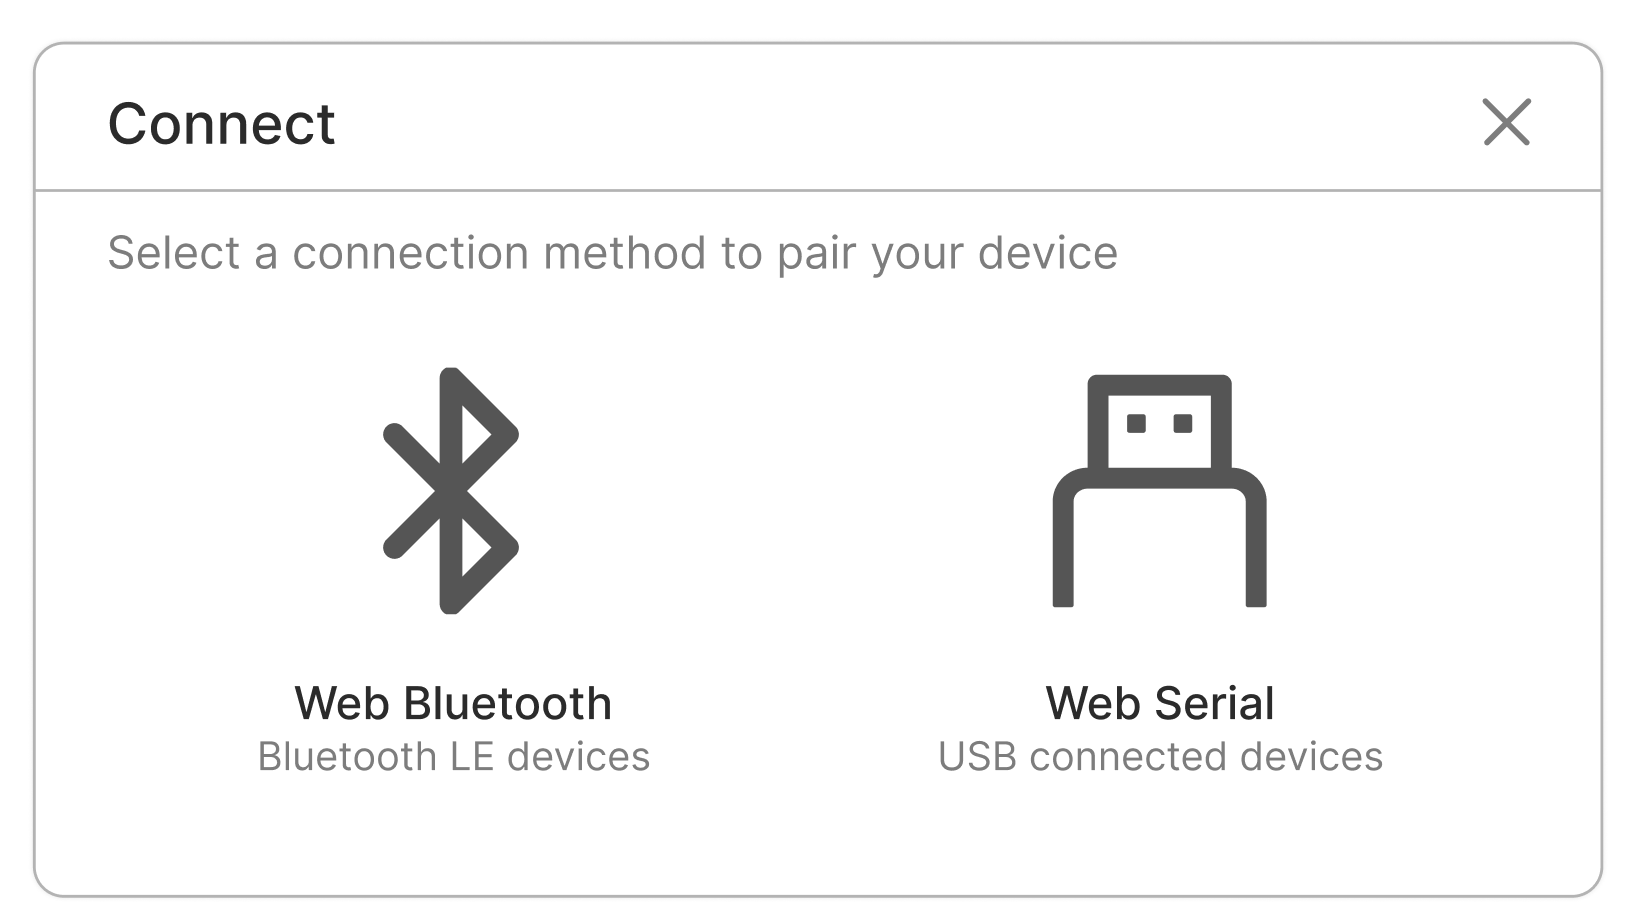
\includegraphics[width=12cm]{dissertation/images/wireframe-connection.png}
    \caption{Proposed modal for device connection, with a design inspired from the React Mantine UI library aiming to make embedding Espruino connection into a web application cleaner and more suited to modern web design.}
    \label{fig:connection-wireframe}
\end{figure}

\begin{figure}[H]
    \centering
    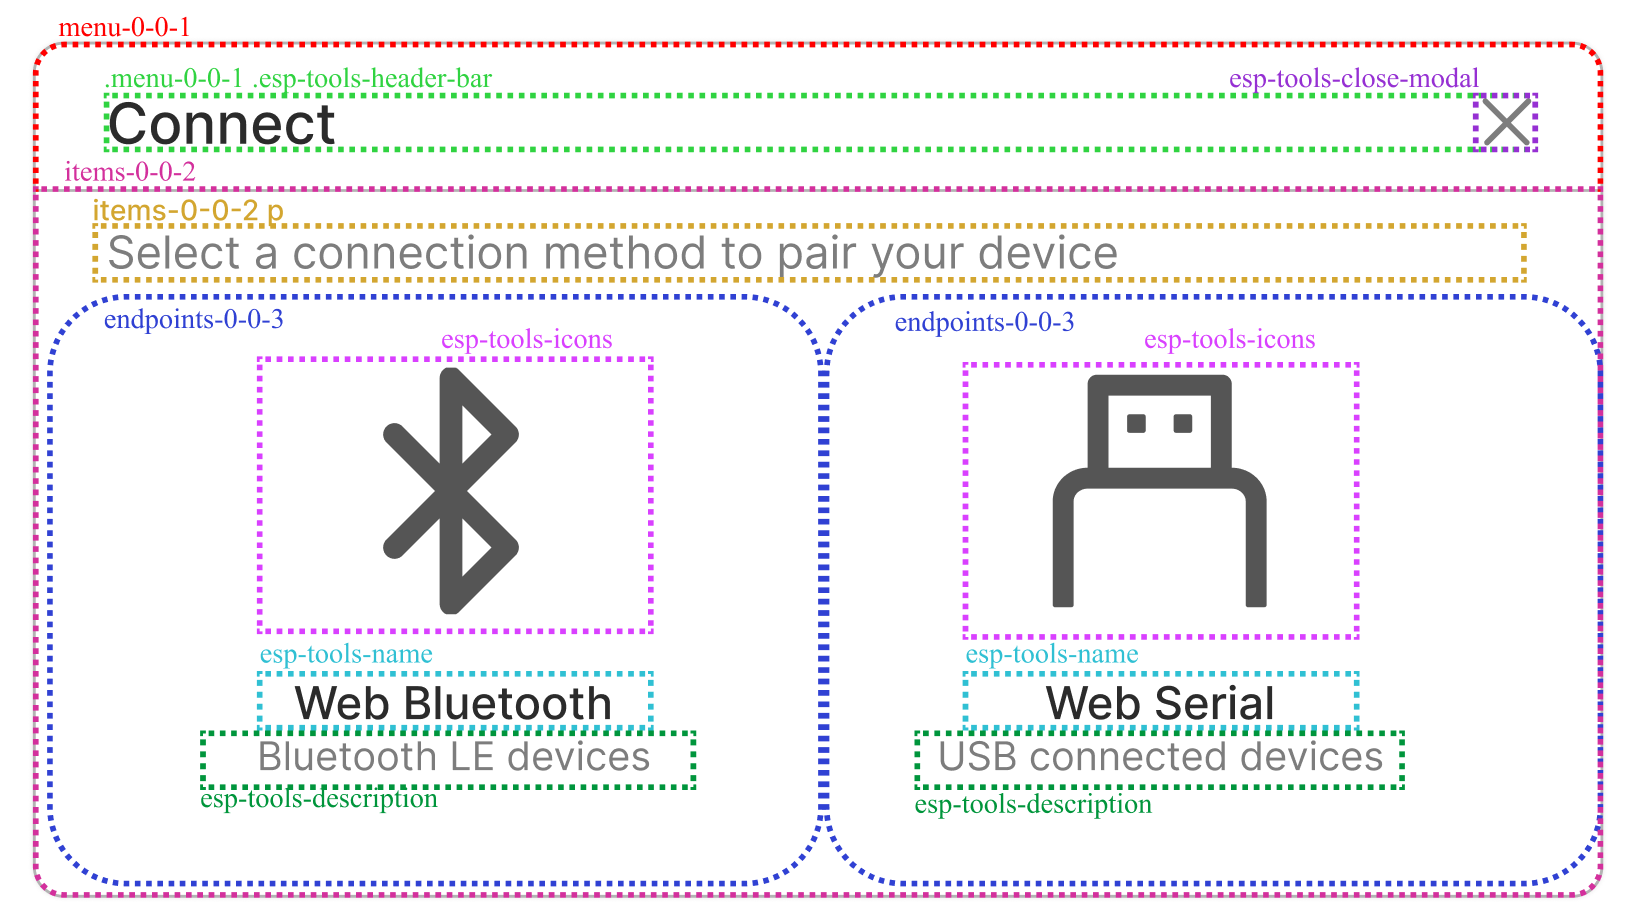
\includegraphics[width=12cm]{dissertation/images/wireframe-connection-style-guide.png}
    \caption{Wireframe for the style guide for the connection modal to allow developers an easy method of restyling to fit their own web pages design. This includes CSS variable names in BEM formatting due to the usage of JSS on the web page.}
    \label{fig:connection-style-wireframe}
\end{figure}

\section{Qr Code}

\begin{figure}[H]
    \centering
    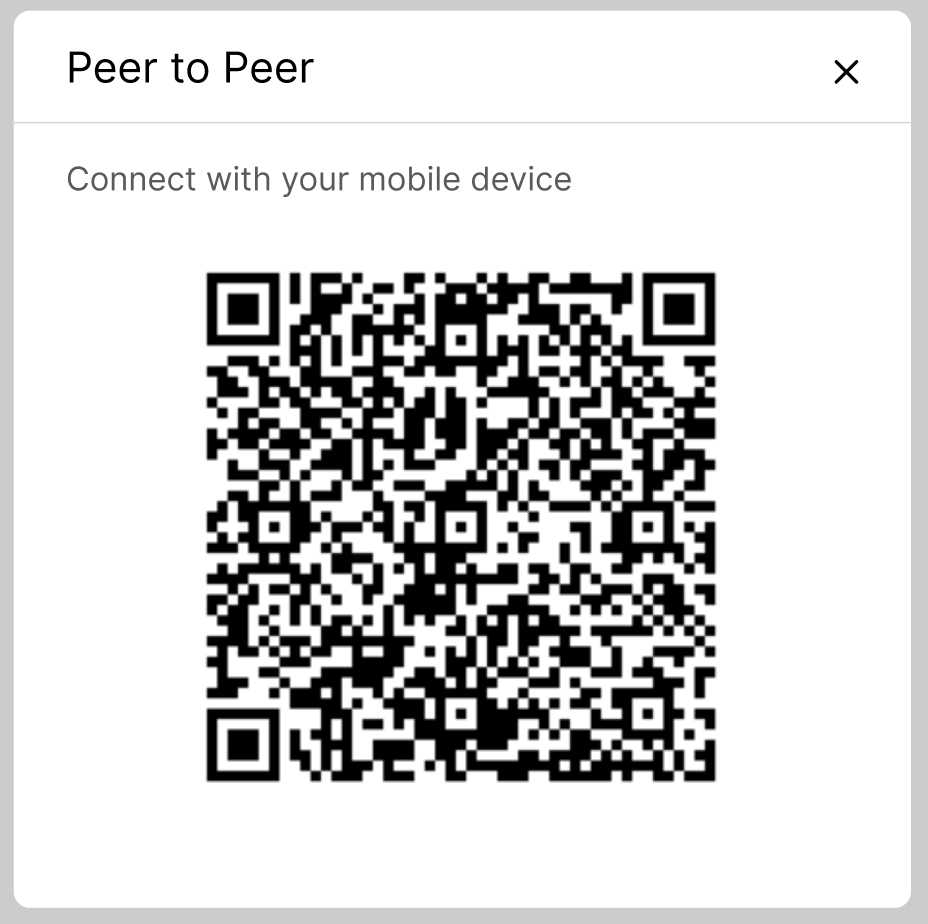
\includegraphics[width=12cm]{dissertation/images/wireframe-qr.png}
    \caption{Proposed modal for peer-to-peer mobile device scanning through the addition of a QR code, styled to be consistent with the connection modal in \ref{fig:connection-wireframe}}
    \label{fig:qr-wireframe}
\end{figure}

\begin{figure}[H]
    \centering
    
\includegraphics{dissertation/images/wireframe-qr-icon.png}
    \caption{Proposed icon to enable to peer-to-peer modal, this was designed to ensure ease of integration into customised website designs whilst being full replaceable if needed}
    \label{fig:qr-icon-wireframe}
\end{figure}

\chapter{Student University Study}

\text The survey gauges how students think the current state of programming education at the University of Glasgow is.

\begin{figure}[!ht]
    \centering
    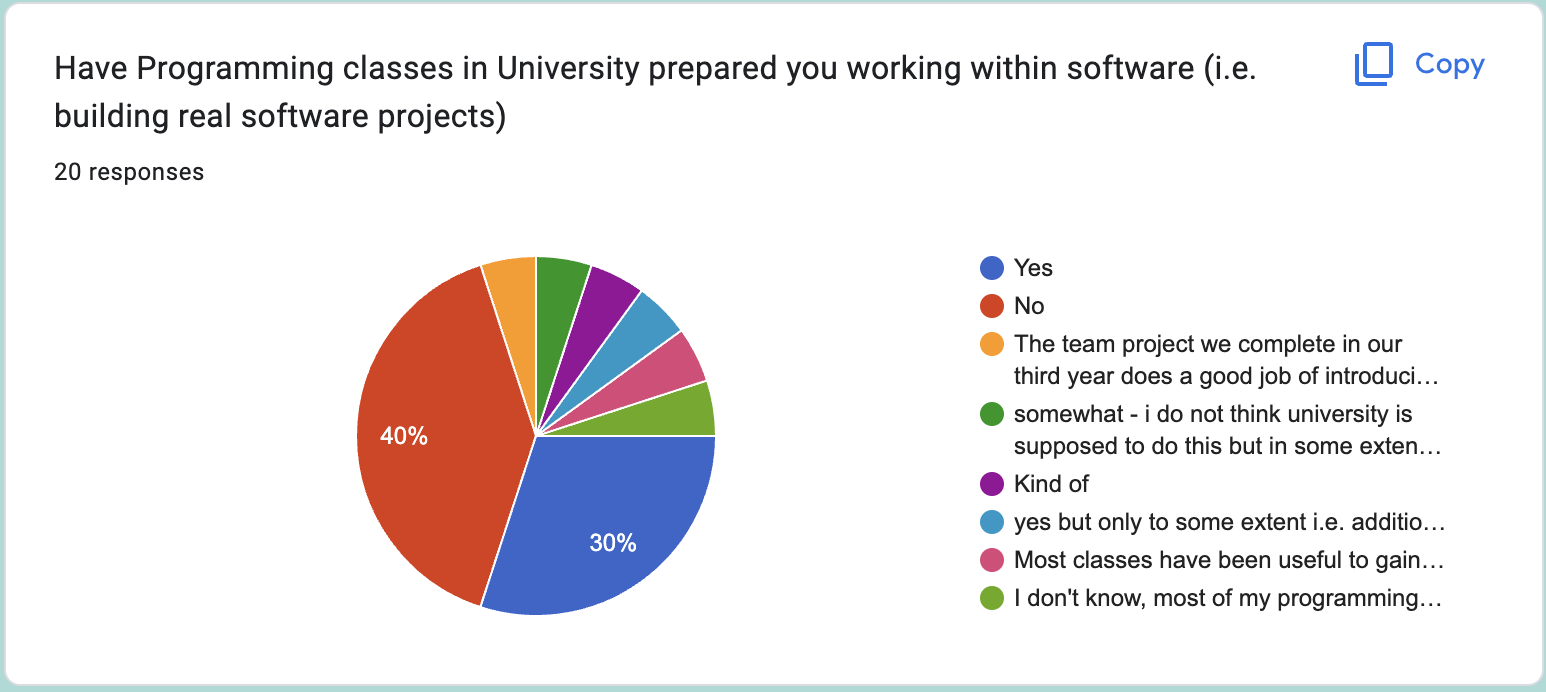
\includegraphics[width=14cm]{dissertation/images/prog-survey-Q1.png}
    \caption{Survey question on whether or not programming classes in university have aided students in developing their own production-grade systems.}
    \label{fig:survey-q1}
\end{figure}

\begin{figure}[!ht]
    \centering
    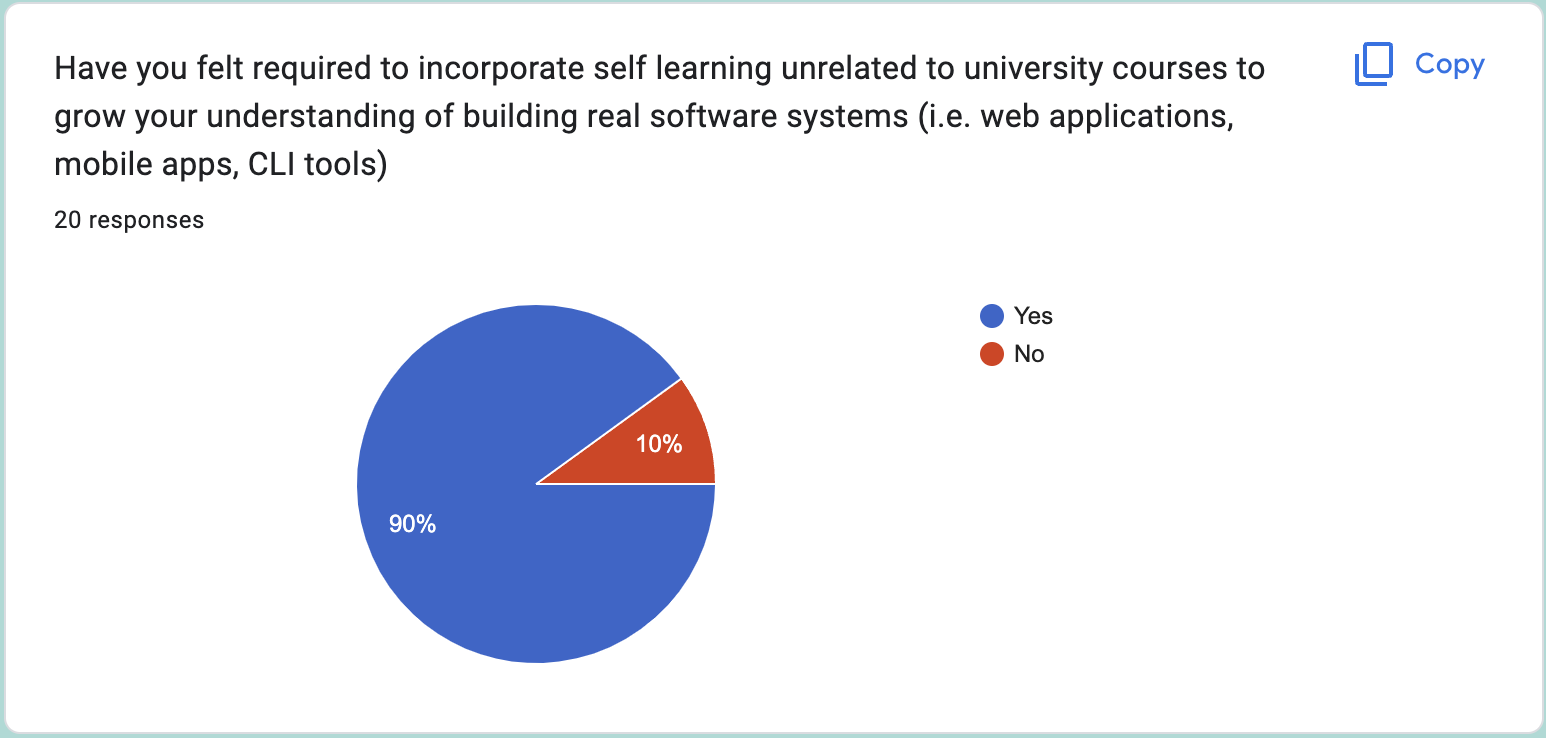
\includegraphics[width=14cm]{dissertation/images/prog-survey-Q2.png}
    \caption{Survey question on whether or not students have had to incorporate self learning into the schedule to keep up with building real software systems such as web or mobile applications}
    \label{fig:survey-q2}
\end{figure}

\begin{figure}[!ht]
    \centering
    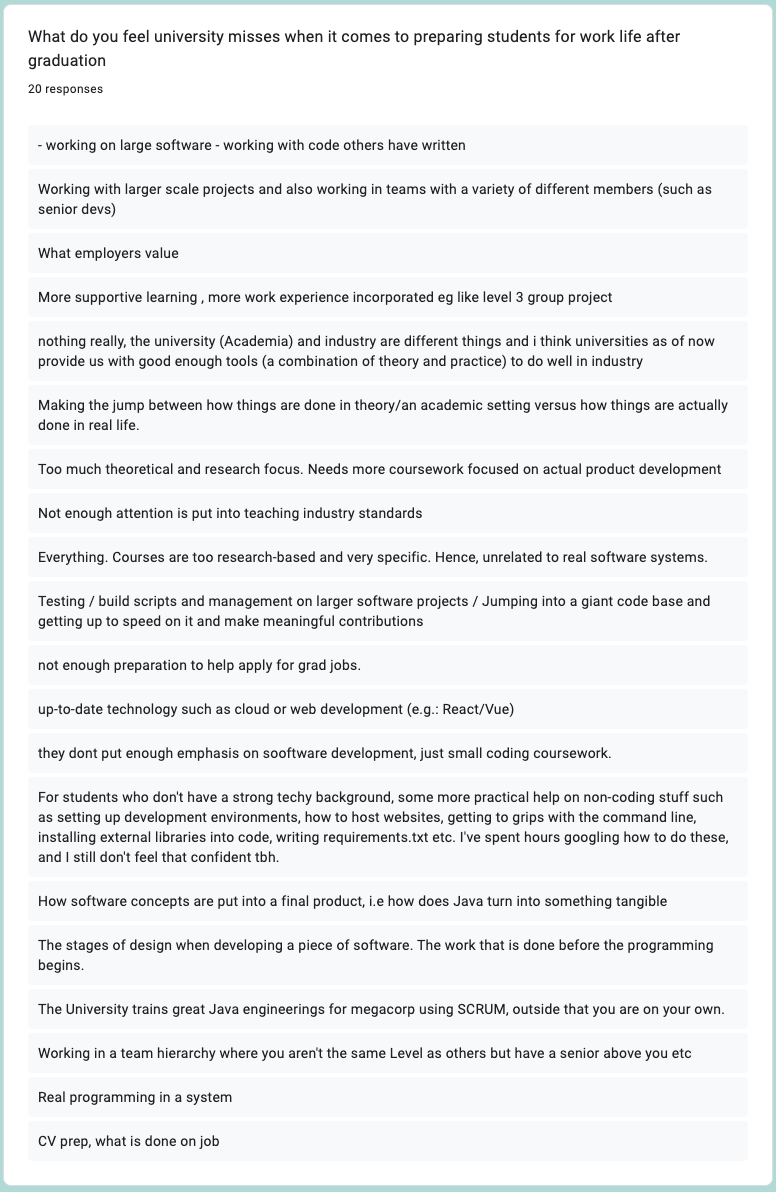
\includegraphics{dissertation/images/prog-survey-Q3.png}
    \caption{An open-ended survey question to gauge what students believe the university misses when it comes to preparing students for their work life after university}
    \label{fig:survey-q3}
\end{figure}

\begin{figure}[!ht]
    \centering
    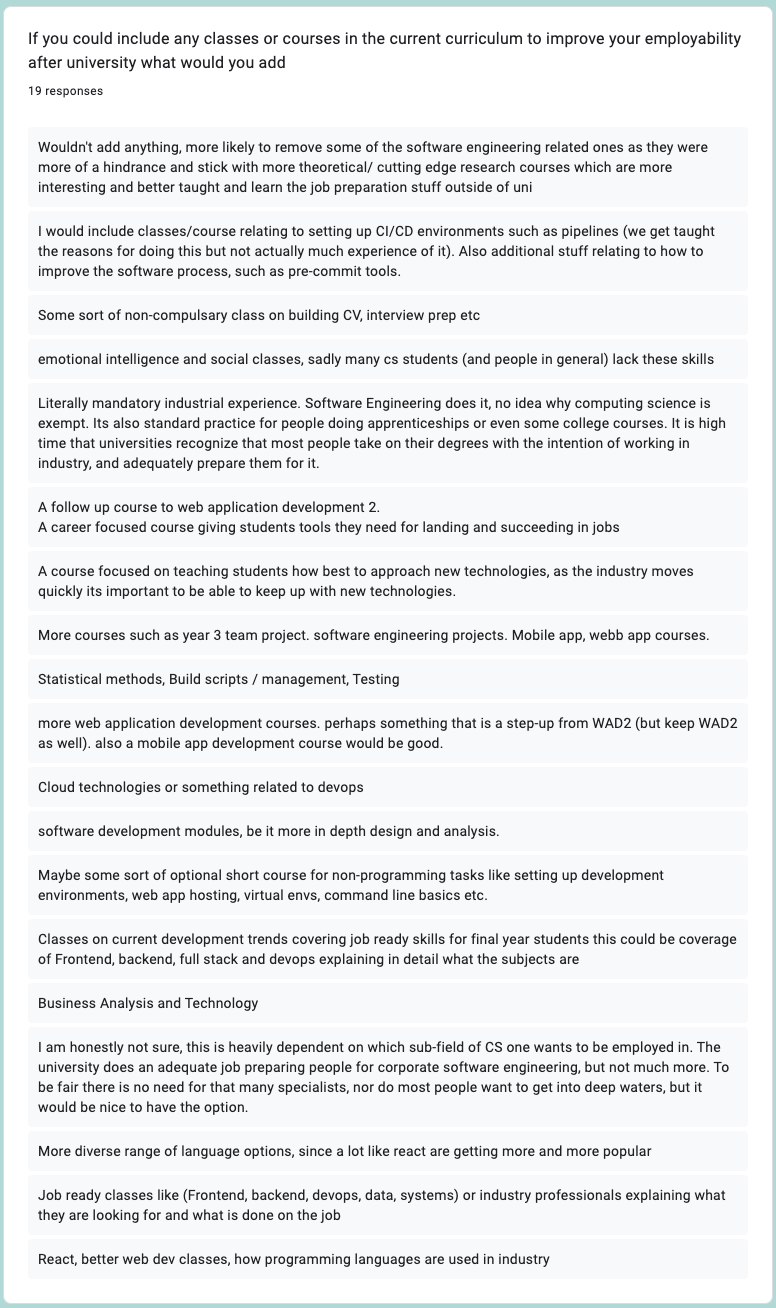
\includegraphics{dissertation/images/prog-survey-Q4.png}
    \caption{An open-ended survey question to gauge what students wish the university had included in the curriculum to prepare them for work after graduation}
    \label{fig:survey-q4}
\end{figure}

\label{appendix:studentunistudy}
\end{appendices}

%==================================================================================================================================
%   BIBLIOGRAPHY   

% The bibliography style is abbreviated
% The bibliography always appears last, after the appendices.

\bibliographystyle{abbrvnat}

\bibliography{l4proj}

\end{document}
